\documentclass[journal]{IEEEtran}

\usepackage{cite}
\usepackage{amsmath,amssymb,amsfonts}
\usepackage{graphicx}
\usepackage{textcomp}
\usepackage{subcaption}
\usepackage{booktabs}
\usepackage{multirow}
\usepackage{microtype}
\usepackage{caption}
\usepackage{balance}
\usepackage{algorithm}
\usepackage{algpseudocode}
\usepackage{siunitx}
\captionsetup{font=small,labelfont=bf}

\graphicspath{{framework/}{representation/}{AW-DPCNN/}{MSCA-VGG16/}{Fused images/}{equipment/}{confusion_matrix/}{tsne/}{tsne_cwru/}{raw_tsne/}{tsne_models/}{figures/}}

\hyphenation{op-tical net-works semi-conduc-tor IEEE-Xplore}

\begin{document}

% \title{AW-DPCNN Based Multi-Representation Supervised Learning for Mechanical Signal Fault Diagnosis}
% \title{AW-DPCNN: Adaptive-Weighted Dual-PCNN Fusion of Time-Frequency Representations for Non-Stationary Fault Diagnosis}
\title{Adaptive Weighted Dual-Channel PCNN Multi-Representation Fusion Network for Vibration Signal Fault Diagnosis}

\author{Chen Yang, Zonglong Bai, Zhiyuan Xie, Chenggang Liu, Junyan Zhang and Yihe Guo}

\markboth{IEEE Transactions on Instrumentation and Measurement}
{Yang~\MakeLowercase{\textit{et al.}}: AW-DPCNN Based Multi-Representation Supervised Learning for Mechanical Signal Fault Diagnosis}

\maketitle

\begin{abstract}
Non-stationary vibration signals from rotating machinery pose significant challenges for intelligent fault diagnosis, as conventional single-representation methods often fail to capture the full spectrum of discriminative fault information. This paper presents an Adaptive Weighted Dual-Channel Pulse-Coupled Neural Network (AW-DPCNN) for multi-representation fusion, coupled with a Multi-Scale Channel Attention enhanced VGG16 (MSCA-VGG16) classifier, to address the limitations of existing approaches in fusing heterogeneous time--frequency and temporal-encoded representations. The AW-DPCNN introduces three key mechanisms: dual-channel external stimuli that independently process time--frequency representations and Gramian Angular Difference Field (GADF) encodings through representation-specific convolutional kernels; a contrast-guided adaptive weighting scheme that dynamically regulates the relative contribution of each representation based on local saliency; and iterative pulse-coupled dynamics that propagate and reinforce structurally consistent features while suppressing spurious activations. The fused representations are then classified by MSCA-VGG16, which integrates multi-scale convolution for capturing fault patterns across different temporal and spectral granularities, squeeze-and-excitation channel attention for dynamic frequency-band recalibration, and a compact discriminative embedding head for enhanced inter-class separation. Extensive experiments on the Case Western Reserve University (CWRU) bearing dataset demonstrate that AW-DPCNN fusion consistently outperforms single-representation baselines and naive concatenation strategies. The full AW-DPCNN and MSCA-VGG16 pipeline achieves 99.19\% accuracy on the 12 kHz drive-end benchmark, with strong generalization to fan-end sensor data (95.33\%) and cross-sampling-rate scenarios (94.81\% at 48 kHz). Comprehensive ablation studies, representation comparisons across twelve time--frequency and temporal encoding combinations, noise robustness evaluations, and hyperparameter sensitivity analyses collectively validate the effectiveness, robustness, and generalizability of the proposed framework for non-stationary mechanical signal fault diagnosis.
\end{abstract}

\begin{IEEEkeywords}
Fault diagnosis, Gramian angular difference field (GADF), multi-representation fusion, pulse coupled neural network (PCNN), rotating machinery, short-time Fourier transform (STFT), time--frequency analysis.
\end{IEEEkeywords}

\section{Introduction}
\IEEEPARstart{R}{otating} machinery, including bearings, gears, and shafts, constitutes the core of modern industrial systems~\cite{10313245},~\cite{10697175}. Unexpected failures of these critical components can lead to catastrophic breakdowns, substantial economic losses, and severe safety hazards. Consequently, reliable and intelligent fault diagnosis techniques have become indispensable for condition-based maintenance and operational safety assurance~\cite{6899683}. Among various diagnostic modalities, vibration-based monitoring has received the most extensive research attention due to its rich fault-related information content, non-intrusive sensor deployment, and well-established physical understanding of fault-induced vibration signatures~\cite{9344691}~\cite{9440949}.

Despite the practical success of vibration-based diagnosis, the non-stationary nature of real-world machinery signals remains a fundamental challenge. Under variable speed, fluctuating load, and time-varying operating conditions, vibration signals exhibit pronounced non-stationary characteristics, as their spectral content and statistical properties evolve over time in complex ways that cannot be adequately captured by conventional stationary signal processing techniques~\cite{8853278}~\cite{9242332}. Single time-domain or frequency-domain representations each capture only partial aspects of these rich signals: time-domain features may overlook critical spectral information, while frequency-domain representations discard temporal evolution patterns that are essential for distinguishing transient fault events from steady-state operating conditions~\cite{8068181}~\cite{10319398}.

To address the limitations of single-representation approaches, researchers have explored complementary representation strategies. Time--frequency representations such as the Short-Time Fourier Transform (STFT) spectrogram, Mel spectrogram, and continuous wavelet transform (CWT) scalogram provide joint time--frequency energy distributions that reveal how spectral content evolves temporally~\cite{10226588},~\cite{10816403},~\cite{9252126}. In parallel, temporal encoding methods such as the Gramian Angular Field (GAF), Markov Transition Field (MTF), and Recurrence Plot (RP) transform one-dimensional time series into two-dimensional images by encoding pairwise temporal relationships, thereby preserving global temporal correlation structures that time--frequency methods may not explicitly capture~\cite{10443404},~\cite{10517915}~\cite{10703061}. However, most existing studies adopt a single representation for downstream classification, and the complementary nature of time--frequency and temporal-encoded representations remains largely underexploited.

Multi-representation fusion offers a natural avenue to combine the strengths of heterogeneous representations, yet existing fusion strategies face critical limitations. Simple concatenation or pixel-wise averaging ignores the distinct statistical properties and structural characteristics of different representations, potentially introducing destructive interference rather than constructive complementarity~\cite{8513874}~\cite{10260234}. Fixed-weight fusion schemes lack the adaptivity to emphasize discriminative representations while suppressing less informative ones on a per-sample or per-region basis~\cite{10265257}. Furthermore, conventional deep learning classifiers, while powerful, often lack explicit architectural mechanisms to exploit the multi-scale and channel-wise characteristics of fused representations~\cite{11345448}~\cite{8788665}.

To address these gaps, this paper proposes a two-stage framework comprising an Adaptive Weighted Dual-branch Pulse-Coupled Neural Network (AW-DPCNN) for multi-representation fusion, and a Multi-Scale Channel Attention enhanced VGG16 (MSCA-VGG16) classifier for robust fault identification. The main contributions are:

\begin{itemize}
\item An AW-DPCNN fusion mechanism is proposed to adaptively integrate time--frequency representations (STFT spectrogram) and temporal-encoded representations (GADF). The mechanism introduces contrast-guided adaptive weighting to dynamically regulate per-channel contributions, dual-channel external stimuli with representation-specific convolutional kernels, and iterative pulse-coupled dynamics for feature reinforcement.

\item An MSCA-VGG16 classification network is constructed to further exploit the complementary information encoded in the fused representations. The architecture integrates multi-scale convolution for capturing fault patterns at multiple temporal and spectral granularities, squeeze-and-excitation channel attention for dynamic frequency-band recalibration, and a compact embedding head for enhanced discriminability.

\item Extensive experiments on the CWRU bearing dataset, including backbone comparisons, comprehensive ablation studies, representation comparisons across twelve time--frequency and temporal encoding combinations, noise robustness evaluations at multiple SNR levels, and hyperparameter sensitivity analyses, systematically validate each component of the proposed framework.

\item Cross-sensor and cross-sampling-rate generalization is demonstrated on the CWRU 12 kHz fan-end and 48 kHz drive-end datasets, confirming the robustness and transferability of the proposed approach beyond the primary benchmark.

\end{itemize}

The remainder of this paper is organized as follows. Section~\ref{section2} reviews related work. Section~\ref{section3} presents the proposed AW-DPCNN fusion mechanism and MSCA-VGG16 classifier. Section~\ref{section4} describes the experimental setup and comprehensive performance evaluation. Finally, conclusions are drawn in Section~\ref{section5}.
\begin{figure*}[!t]
\centering
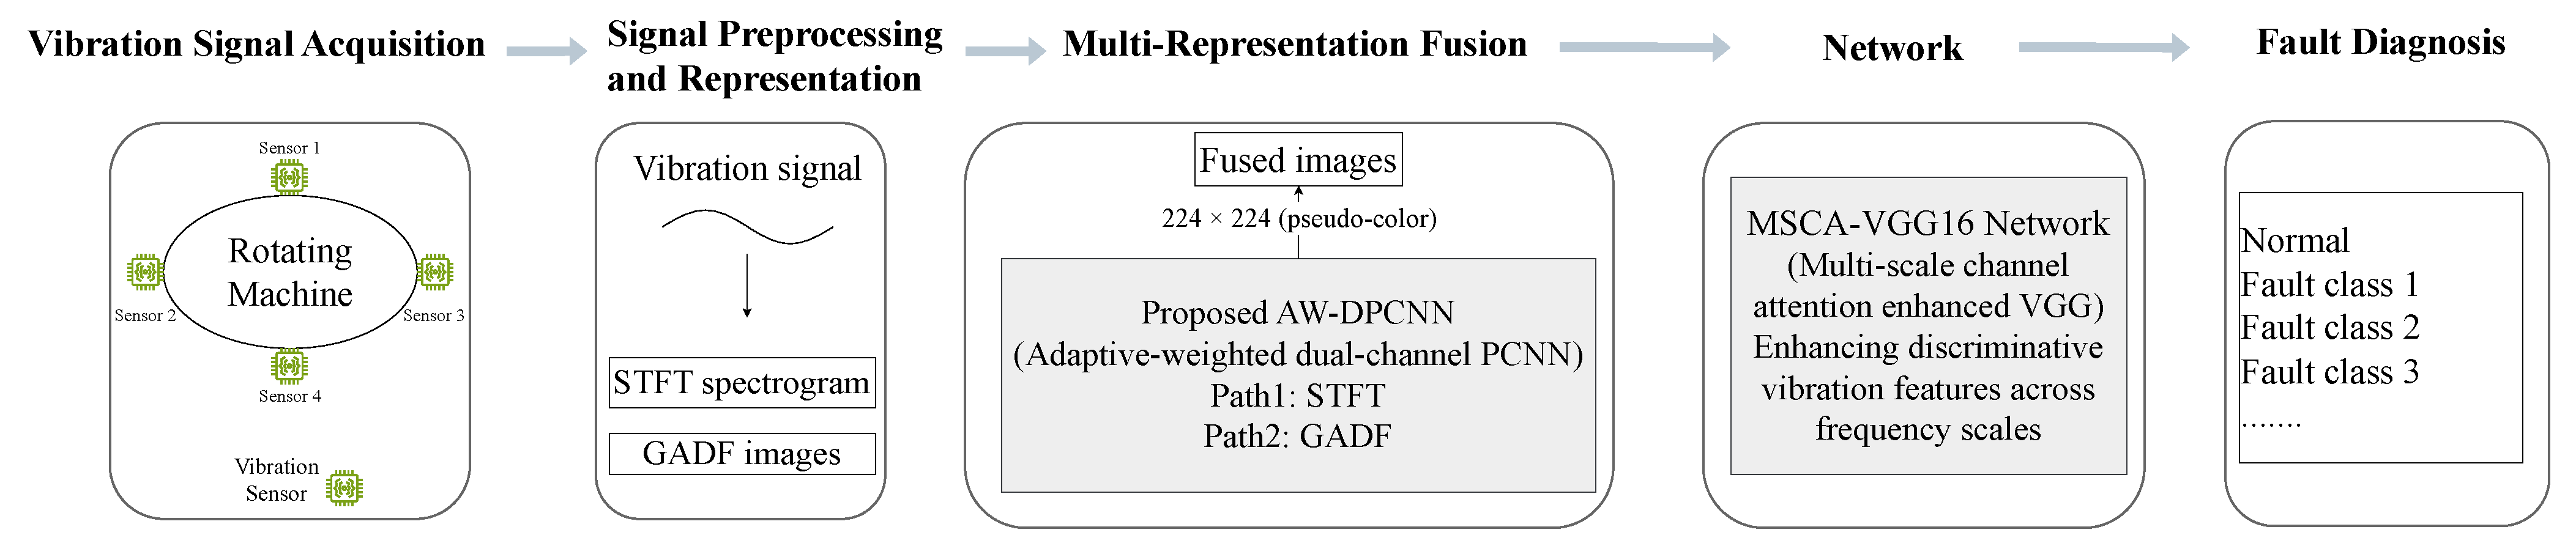
\includegraphics[width=\linewidth]{framework/framework1}
\caption{Overall framework of the proposed vibration signal fault diagnosis method. The vibration signal is first converted into STFT spectrogram and GADF images. These heterogeneous representations are then adaptively fused through the proposed AW-DPCNN mechanism. Finally, the fused feature is fed into the MSCA-VGG16 network for fault classification.}
\label{framework}
\end{figure*}

\section{Related Work}
\label{section2}

\subsection{Signal Representations for Fault Diagnosis}

Time--frequency representations have been extensively applied to vibration-based
bearing fault diagnosis. STFT spectrograms combined with 2-D CNNs have demonstrated
effective classification of bearing defects by converting raw vibration signals into
time--frequency images that convolutional architectures can process~\cite{11028059},
\cite{10623182}. CWT scalograms have been employed to achieve improved time--frequency
localization for transient fault signatures, with multi-resolution analysis offering
advantages over fixed-resolution STFT for certain non-stationary conditions~\cite{11028613}.
Mel spectrograms have also been explored for their perceptually motivated frequency
compression, particularly for harmonic-rich fault patterns~\cite{10929672}. Despite
these successes, time--frequency representations fundamentally characterize local
spectral energy distributions and do not explicitly model long-range temporal
dependencies that may contain complementary diagnostic information.

In a parallel direction, temporal encoding methods have been introduced to transform
one-dimensional vibration signals into two-dimensional images that preserve pairwise
temporal relationships. Xiong et al. applied GAF encoding to complementary ensemble empirical mode decomposition-preprocessed vibration signals, enabling CNN-based classification of the resulting temporal correlation images~\cite{10109681}. MTF and RP encodings have similarly been adopted to
capture sequential transition dynamics and recurrent phase-space patterns,
respectively~\cite{11303191},~\cite{10684078}. However, these temporal encoding methods primarily preserve correlation
structures and lack explicit frequency-domain specificity, which is critical for
distinguishing faults with similar temporal patterns but distinct spectral signatures.

A limited number of recent studies have explored combining multiple representations
for fault diagnosis. Representative efforts include channel-wise concatenation of
time--frequency and temporal-encoded images for CNN-based classification, and
pixel-level averaging of complementary representation pairs~\cite{10214203},~\cite{11538063}. However, these approaches
employ fixed fusion strategies that treat all spatial locations and feature channels
uniformly, without adaptively regulating the relative contribution of each
representation. Given that time--frequency and temporal-encoded representations
possess fundamentally different statistical properties and structural characteristics,
naive fusion may introduce destructive interference rather than constructive
complementarity. The systematic exploration and
adaptive fusion of heterogeneous representations for vibration signal fault diagnosis therefore
remains an open research problem, motivating the AW-DPCNN framework proposed in this
work.

\subsection{PCNN and Multi-Representation Fusion}
Pulse-coupled neural networks (PCNNs) are neural models originally developed to simulate the synchronous firing behavior observed in the mammalian visual cortex \cite{761706}. Unlike conventional convolutional neural networks, PCNNs employ a pulse-based activation mechanism in which neurons interact through local coupling and dynamic thresholds \cite{761716}. Owing to these characteristics, PCNNs exhibit strong capability in preserving structural information while suppressing background interference, and have been widely applied in image segmentation, edge detection, and feature enhancement tasks~\cite{1427771},~\cite{8742596},~\cite{9444355}. 

However, conventional PCNNs are typically driven by a single external stimulus, which limits their ability to effectively exploit complementary information from multiple representations. To address this limitation, dual-channel PCNN (DPCNN) architectures have been introduced to enable multi-representation fusion by incorporating multiple external stimuli within the neuronal feeding mechanism, and later extended with adaptive parameter estimation via fractal dimension to eliminate manual tuning~\cite{9072551}. Through this mechanism, heterogeneous feature maps can be jointly processed, thereby facilitating the integration of information from different representations. Nevertheless, the fusion process in such architectures generally relies on fixed or predefined coupling strategies, making it difficult to adaptively regulate the relative contributions of different channels. As a result, the model may not effectively emphasize discriminative representations while suppressing less relevant ones, thereby limiting the effectiveness of multi-representation fusion. Although DPCNN-based fusion has been preliminarily explored in image processing, its application to machinery fault diagnosis, where heterogeneous time--frequency and temporal-encoded representations must be jointly exploited, remains largely uninvestigated.

\subsection{Deep Learning for Fault Diagnosis}

With the rapid advancement of deep learning techniques, a variety of neural network architectures have been applied to vibration signal fault diagnosis, demonstrating superior automatic feature extraction capability compared with traditional handcrafted methods~\cite{8945322},~\cite{11435266}. Early studies commonly adopted baseline convolutional neural networks as benchmark architectures for acoustic and vibration fault classification, verifying the feasibility of end-to-end feature learning for fault diagnosis tasks \cite{9770836}. Subsequently, classical deep convolutional backbones, including EfficientNet, ViT, MobileNet, ConvNeXt and ResNet, were introduced into intelligent fault diagnosis frameworks and achieved notable improvements in hierarchical feature representation and classification accuracy across machinery health monitoring applications~\cite{11028988},~\cite{10663388},~\cite{9374431}. Among these, VGG16's purely sequential topology with no skip connections or built-in attention mechanisms provides a clean architectural foundation for attaching auxiliary modules such as multi-scale convolution and channel attention, making it particularly suitable as a backbone for the MSCA enhancement strategy pursued in this work~\cite{10048773}. More recently, advanced architectures such as ConvNeXt, which incorporate modernized convolutional design principles, have further enhanced representation learning capability and demonstrated competitive performance in fault diagnosis and image-based classification tasks~\cite{10980179}. In addition, publicly available benchmark datasets, such as the CWRU bearing fault dataset, have been extensively employed to evaluate the effectiveness and generalization ability of deep learning-based diagnostic models, serving as a standard reference in fault diagnosis research \cite{SMITH2015100}.

Despite these advances, most existing deep learning approaches for fault diagnosis are designed to process a single input representation and lack dedicated architectural mechanisms, such as multi-scale receptive fields and dynamic channel attention, for jointly exploiting the heterogeneous features produced by multi-representation fusion. Consequently, their capacity to fully leverage the complementary information encoded in fused time--frequency and temporal representations remains limited, motivating the design of the MSCA-VGG16 classifier proposed in this work.

\section{Methodology}
\label{section3}

\subsection{Overview}
The proposed framework comprises two sequential stages: multi-representation signal fusion and fused representation classification, as illustrated in Fig.~\ref{framework}. In the fusion stage, the raw vibration signal is first transformed into two complementary representations, namely the STFT spectrogram and the Gramian Angular Difference Field (GADF) image, to capture time--frequency energy distributions and global temporal correlation structures, respectively. These heterogeneous representations are then adaptively integrated through the proposed AW-DPCNN mechanism, which employs contrast-guided adaptive weighting and dual-channel pulse-coupled dynamics to produce a unified fused representation. In the classification stage, the fused representation is fed into the MSCA-VGG16 network, which incorporates multi-scale convolution and channel attention to enhance feature discrimination, followed by a compact embedding head for robust fault classification.

Formally, let $\boldsymbol{x} \in \mathbb{R}^{L}$ denote a raw vibration signal segment of length $L$. The signal is first mapped to two heterogeneous representations as
\begin{equation}
\boldsymbol{S}_{\mathrm{STFT}} = \mathcal{T}_{\mathrm{STFT}}(\boldsymbol{x}), \quad
\boldsymbol{S}_{\mathrm{GADF}} = \mathcal{T}_{\mathrm{GADF}}(\boldsymbol{x}),
\label{eq:pipeline_rep}
\end{equation}
where $\mathcal{T}_{\mathrm{STFT}}(\cdot)$ and $\mathcal{T}_{\mathrm{GADF}}(\cdot)$ denote the STFT spectrogram and GADF transformation operators, respectively, both producing pseudo-color RGB images. The two representations are then fused via the AW-DPCNN operator $\mathcal{F}_{\mathrm{AW}}(\cdot, \cdot)$ as
\begin{equation}
\boldsymbol{S}_{\mathrm{fused}} = \mathcal{F}_{\mathrm{AW}}(\boldsymbol{S}_{\mathrm{STFT}}, \boldsymbol{S}_{\mathrm{GADF}}; \Theta_{\mathrm{AW}}),
\label{eq:pipeline_fuse}
\end{equation}
where $\Theta_{\mathrm{AW}}$ denotes the set of AW-DPCNN hyperparameters. Finally, the fused representation is passed through the MSCA-VGG16 classifier $\mathcal{C}(\cdot)$ to produce the predicted fault class probabilities
\begin{equation}
\hat{\boldsymbol{y}} = \mathcal{C}(\boldsymbol{S}_{\mathrm{fused}}; \Theta_{\mathrm{CLS}}),
\label{eq:pipeline_cls}
\end{equation}
where $\Theta_{\mathrm{CLS}}$ denotes the trainable parameters of the classification network and $\hat{\boldsymbol{y}} \in \mathbb{R}^{K}$ is the predicted probability vector over $K$ fault categories. The following subsections detail each component of this pipeline.

\subsection{Signal Representation}

The raw vibration signal segment $\boldsymbol{x} \in \mathbb{R}^{L}$, introduced in~\eqref{eq:pipeline_rep}, serves as the common input from which both representations are derived. The STFT spectrogram $\boldsymbol{S}_{\mathrm{STFT}}$ captures local time--frequency energy distributions through short-time spectral analysis, while the GADF image $\boldsymbol{S}_{\mathrm{GADF}}$ encodes global temporal correlation structures through pairwise angular relationships. Their respective constructions are detailed below.

\subsubsection{STFT Spectrogram}

The STFT spectrogram is a linear time--frequency representation that preserves uniform frequency resolution across the entire spectrum. Let $x[k]$ denote the $k$-th sample of the vibration signal segment $\boldsymbol{x}$. The construction involves dividing $\boldsymbol{x}$ into overlapping frames of length $n_{\mathrm{fft}}$, applying a Hann window $w(\cdot)$ to each frame, and computing the discrete Fourier transform. The magnitude spectrum of each frame is arranged chronologically to form a two-dimensional time--frequency representation $\boldsymbol{S}_{\mathrm{STFT}}(t, f)$, defined as
\begin{equation}
\boldsymbol{S}_{\mathrm{STFT}}(t, f) = \left| \sum_{k=0}^{n_{\mathrm{fft}}-1} x[k] \, w(k - t) \, e^{-j 2\pi f k / n_{\mathrm{fft}}} \right|^2.
\label{eq:stft}
\end{equation}

The STFT spectrogram is parameterized by the FFT window size $n_{\mathrm{fft}}$ and hop length $n_{\mathrm{hop}}$, which jointly determine the temporal resolution and frequency resolution $\Delta f = f_s / n_{\mathrm{fft}}$ at a given sampling rate $f_s$.

\begin{figure}[!t]
	\centering
	\graphicspath{{representation/}}
	\begin{subfigure}{0.48\linewidth}
		\centering
		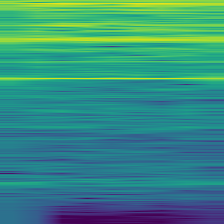
\includegraphics[width=\linewidth]{STFT_98_Normal_1_00000}
		\caption{STFT spectrogram}
	\end{subfigure}
	\hfill
	\begin{subfigure}{0.48\linewidth}
		\centering
		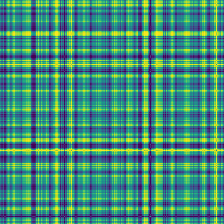
\includegraphics[width=\linewidth]{GADF_98_Normal_1_00000}
		\caption{GADF}
	\end{subfigure}
	
	\caption{Vibration signal representations. (a) STFT spectrogram. (b) GADF image.}
	\label{representation}
	
\end{figure}

\subsubsection{Gramian Angular Field}

% To address the limitations of the STFT spectrogram in encoding global temporal structures, the Gramian Angular Field (GAF) is introduced as a complementary representation. 
The GAF transforms the same vibration signal segment $\boldsymbol{x}$ into a two-dimensional image that preserves temporal correlation information through pairwise angular encoding. Let $x_i$ denote the $i$-th sample of $\boldsymbol{x}$. For the purpose of GADF construction, a sequence of $n$ samples $\{x_1, x_2, \ldots, x_n\}$ drawn from $\boldsymbol{x}$ is first normalized to $[-1, 1]$ via min--max scaling,
\begin{equation}
\tilde{x}_i = \frac{(x_i - \min_i x_i) + (x_i - \max_i x_i)}
{\max_i x_i - \min_i x_i}.
\label{normalization}
\end{equation}

The normalized values are then mapped to polar coordinates, where each $\tilde{x}_i$ is encoded as an angular coordinate $\phi_i$ and its temporal position is preserved as the radial coordinate $r_i$,
\begin{equation}
\begin{cases} 
\phi_i = \arccos(\tilde{x}_i), & -1 \leq \tilde{x}_i \leq 1 \\[4pt]
r_i = \dfrac{i}{n}, & i = 1, \ldots, n 
\end{cases}.
\label{cosine angle}
\end{equation}


This polar encoding ensures that the temporal ordering of the signal is preserved through the radial coordinate, while signal amplitude variations are encoded as angular deviations. Finally, pairwise angular differences or sums are aggregated to form the Gramian Angular Summation Field (GASF) and Gramian Angular Difference Field (GADF). The GADF variant,
\begin{equation}
\boldsymbol{G_d}(i,j) = \sin(\phi_i - \phi_j), \quad i,j = 1,\ldots,n,
\label{eq:gadf}
\end{equation}
is adopted in this study due to its higher sensitivity to abrupt temporal variations.

The GAF representation offers several advantages that complement the STFT spectrogram. First, by encoding pairwise angular relationships between all time points, the GAF captures global temporal correlation structures that extend beyond the local receptive field of STFT-based representations. Second, the min--max normalization in~\eqref{normalization} inherently suppresses the influence of absolute signal amplitude, making the GAF representation more robust to variations in signal gain and background noise levels. Furthermore, the polar encoding in~\eqref{cosine angle} provides a bijective mapping, ensuring that temporal information is preserved without loss. 
% As illustrated in Fig.~\ref{representation}(b), the GADF encodes structured temporal dependencies, exhibiting regular and symmetric patterns that reflect stable temporal correlations.

Both representations are subsequently converted to pseudo-color RGB images of spatial dimensions $H \times W$ for compatibility with standard CNN input architectures, through logarithmic amplitude compression and colormap mapping. Fig.~\ref{representation} illustrates representative examples of the STFT spectrogram and GADF image. The concrete parameter values, including $n_{\mathrm{fft}}$, $n_{\mathrm{hop}}$, $f_s$, $n$, $H$, and $W$, are provided in Section~\ref{Dataset Construction and Preprocessing}.

% In this study, the GADF variant is specifically adopted to complement the STFT spectrogram. Compared with GASF, GADF focuses on angular differences and thereby exhibits higher sensitivity to abrupt temporal variations and asymmetric dynamic patterns. This property is particularly beneficial for bearing fault diagnosis, where abnormal operating conditions produce irregular temporal fluctuations in vibration signals. 



\subsection{AW-DPCNN for Multi-Representation Fusion}
\label{sec:awdpcnn}

Owing to their distinct statistical properties and structural characteristics, directly combining the STFT spectrogram and GADF image using conventional pixel-wise averaging or simple feature concatenation may introduce destructive interference rather than constructive complementarity, as demonstrated in the ablation study (Section~\ref{section4}). To address this issue, the proposed AW-DPCNN introduces a PCNN-inspired fusion mechanism with three key innovations: (i) dual-channel external stimuli that independently process STFT and GADF representations through representation-specific convolutional kernels; (ii) a contrast-guided adaptive weighting scheme that dynamically adjusts the relative contribution of each representation based on local saliency; and (iii) iterative pulse-coupled dynamics that propagate and reinforce structurally consistent features across multiple iterations while suppressing spurious activations. The key hyperparameters of the AW-DPCNN are summarized in Table~\ref{tab:awdpcnn_params}, and the detailed formulation of each component is presented below.

\subsubsection{Input Normalization}
To eliminate scale differences between two representations, each input is first normalized to the interval $[0,1]$ as
\begin{equation}
	\boldsymbol{\tilde{S}}_k(i,j) = \frac{\boldsymbol{S}_k(i,j) - \min\limits_{i,j} (\boldsymbol{S}_k(i,j))}{\max\limits_{i,j} (\boldsymbol{S}_k(i,j)) - \min\limits_{i,j} (\boldsymbol{S}_k(i,j)) + \epsilon}, \quad k\in\{1,2\}
	\label{eq:aw_input_norm}
\end{equation}
where $\boldsymbol{S}_1$ and $\boldsymbol{S}_2$ denote the STFT spectrogram and GADF image, respectively, and $\epsilon$ is a small positive constant.

\subsubsection{Contrast-Guided Adaptive Weighting}
For each representation, the local mean of the normalized representation is computed as
\begin{equation}
	\boldsymbol{\mu}_k(i,j) = \frac{1}{|\boldsymbol{\Omega}|}
	\sum_{(p,q)\in \boldsymbol{\Omega}} \boldsymbol{\tilde{S}}_k(p,q),
	\label{eq:local_mean}
\end{equation}
where $\boldsymbol{\Omega}$ denotes the local neighborhood centered at each pixel location, and $|\boldsymbol{\Omega}|$ represents the number of elements in the neighborhood.

The corresponding local contrast is defined as the local standard deviation
\begin{equation}
	C_k(i,j) = \sqrt{ \left| \mathbb{E}_\Omega \left[ \tilde{S}_k^2 \right] - \mu_k^2(i,j) \right| },
	\label{eq:local_contrast}
\end{equation}
where $\mathbb{E}_\Omega[\cdot]$ denotes local averaging within $\boldsymbol{\Omega}$. A contrast amplification factor $\gamma$ is then introduced to construct adaptive fusion weights
\begin{equation}
	\beta_1(i,j) = 
	\frac{\gamma C_1(i,j)}
	{\gamma C_1(i,j) + C_2(i,j) + \epsilon},
	\label{eq:beta1}
\end{equation}
\begin{equation}
	\beta_2(i,j) = 
	\frac{C_2(i,j)}
	{\gamma C_1(i,j) + C_2(i,j) + \epsilon},
	\label{eq:beta2}
\end{equation}
the above formulation ensures $\beta_1(i,j) + \beta_2(i,j) \approx 1$, enabling contrast-driven dynamic weighting.

\subsubsection{Dual-Channel PCNN}
Let $\boldsymbol{L}^n(i,j)$, $\boldsymbol{T}^n(i,j)$, and $\boldsymbol{Y}^n(i,j)$ denote the linking term, dynamic threshold, and binary pulse output, respectively, where $n$ denotes the current iteration and $n \in [1, N]$, with $N$ being the total number of iterations. The neural states are initialized as
\begin{equation}
	\boldsymbol{L}^0(i,j) = \boldsymbol {0}, \quad 
	\boldsymbol{T}^0(i,j) = \boldsymbol {0}, \quad 
	\boldsymbol{Y}^0(i,j) = \boldsymbol {0}.
	\label{eq:initialization}
\end{equation}

At the $n$-th iteration, the external stimulus from two channels is defined as
\begin{equation}
	\boldsymbol{F}_1^n(i,j) = (\boldsymbol{W}_1 * \boldsymbol{Y}^{n-1})(i,j) + \boldsymbol{\tilde{S}}_1(i,j)
	\label{eq:f1_update}
\end{equation}
\begin{equation}
	\boldsymbol{F}_2^n(i,j) = (\boldsymbol{W}_2 * \boldsymbol{Y}^{n-1})(i,j) + \boldsymbol{\tilde{S}}_2(i,j),
	\label{eq:f2_update}
\end{equation}
where $\boldsymbol{W}_1$ and $\boldsymbol{W}_2$ are representation-specific convolutional kernels: stripe-shaped kernels for the STFT channel to emphasize frequency continuity, and symmetric kernels for the GADF channel to capture temporal correlations, and $*$ denotes convolution.

The internal linking state is updated by
\begin{equation}
	\boldsymbol{L}^n(i,j) = e^{-\alpha_L} \boldsymbol{L}^{n-1}(i,j) + (\boldsymbol{M} * \boldsymbol{Y}^{n-1})(i,j),
	\label{eq:linking_update}
\end{equation}
where $\alpha_L$ is the decay coefficient and $\boldsymbol M$ represents the coupling matrix.

The total neuron input is then given by
\begin{equation}
	\boldsymbol{U}^n(i,j) = \big(1 + \boldsymbol{L}^n(i,j)\big)\Big(1 + \beta_1 \boldsymbol{F}_1^n(i,j)\Big)
	\Big(1 + \beta_2 \boldsymbol{F}_2^n(i,j)\Big) + \sigma,
	\label{eq:internal_activity}
\end{equation}
where $\sigma$ is a stabilization constant.

The pulse output is determined by a threshold comparison as follows
\begin{equation}
	\boldsymbol{Y}^n(i,j) =
	\begin{cases}
		1, & \boldsymbol{U}^n(i,j) > \boldsymbol{T}^{n-1}(i,j) \\
		0, & \text{otherwise}
	\end{cases}.
	\label{eq:pulse_output}
\end{equation}

The dynamic threshold evolves according to
\begin{equation}
	\boldsymbol{T}^n(i,j) = e^{-\alpha_T} \boldsymbol{T}^{n-1}(i,j) + V_T \boldsymbol{Y}^n(i,j),
	\label{eq:threshold_update}
\end{equation}
where $\alpha_T$ controls threshold decay and $V_T$ is the amplification coefficient.

\subsubsection{Fused Representation}
The accumulated neural response after $N$ iterations is
\begin{equation}
	\boldsymbol{U}_{\mathrm{sum}}(i,j)=\sum_{n=1}^{N} \boldsymbol{U}^{n}(i,j),
\end{equation}
and the final fused representation is obtained via normalization as
\begin{equation}
	\boldsymbol{F}(i,j)=
	\frac{\boldsymbol{U}_{\mathrm{sum}}(i,j)-\min\limits_{i,j} \boldsymbol{U}_{\mathrm{sum}}(i,j)}
	{\max\limits_{i,j} \boldsymbol{U}_{\mathrm{sum}}(i,j)-\min\limits_{i,j} \boldsymbol{U}_{\mathrm{sum}}(i,j)+\epsilon}.
\end{equation}

The overall architecture of the proposed AW-DPCNN is illustrated in Fig.~\ref{AW-DPCNN}. The qualitative effectiveness of the adaptive fusion mechanism is further analyzed through feature visualization in Section~\ref{section4}.
\begin{figure}[!t]
	\centering
	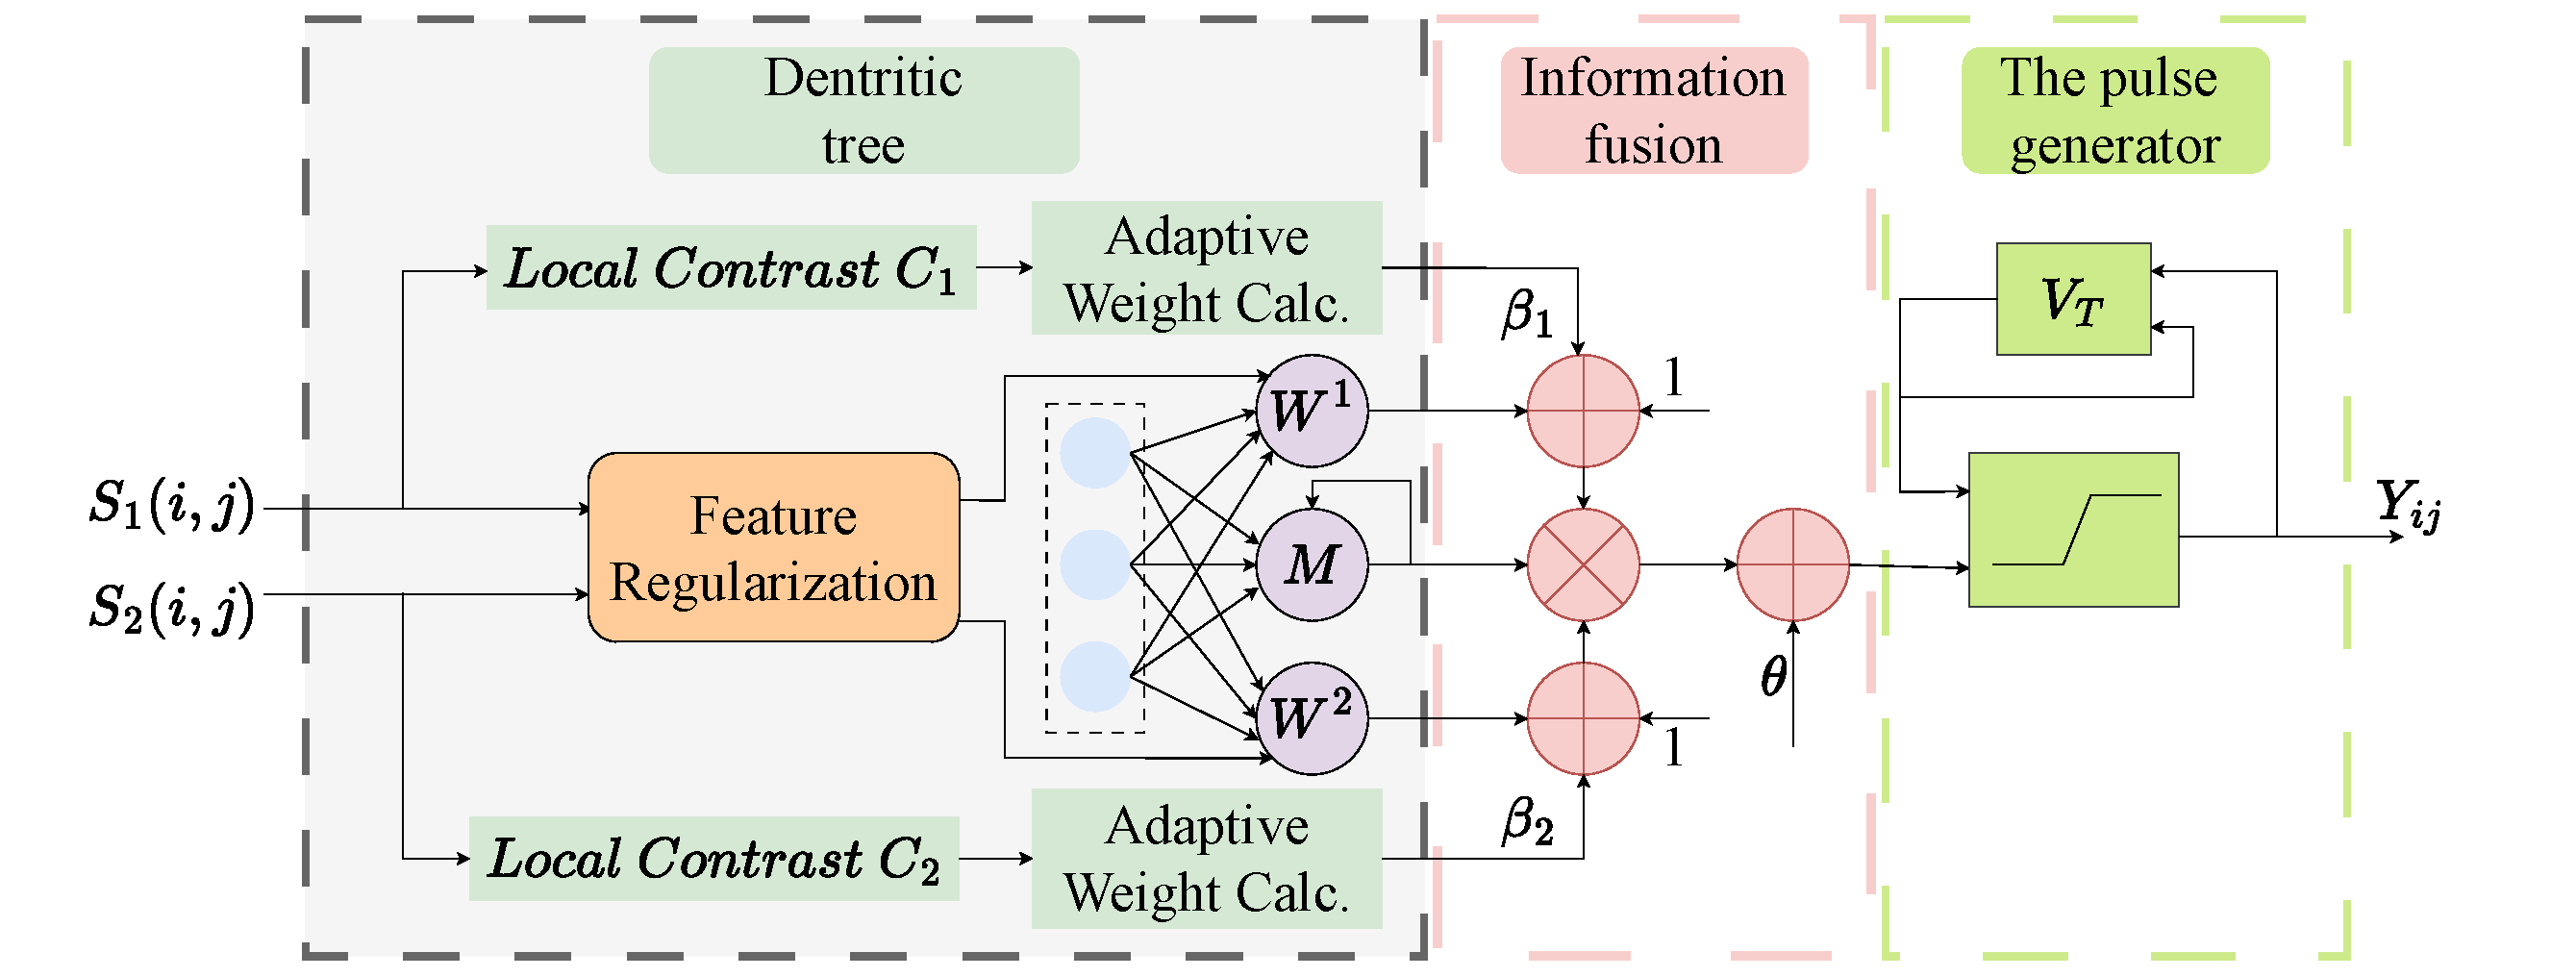
\includegraphics[width=\linewidth]{AW-DPCNN/AW-DPCNN}
	\caption{Architecture of the proposed adaptive weighted dual-channel PCNN (AW-DPCNN) for multi-representation signal fusion.}
	\label{AW-DPCNN}                       
\end{figure}


\begin{figure*}[!t] 
\centering
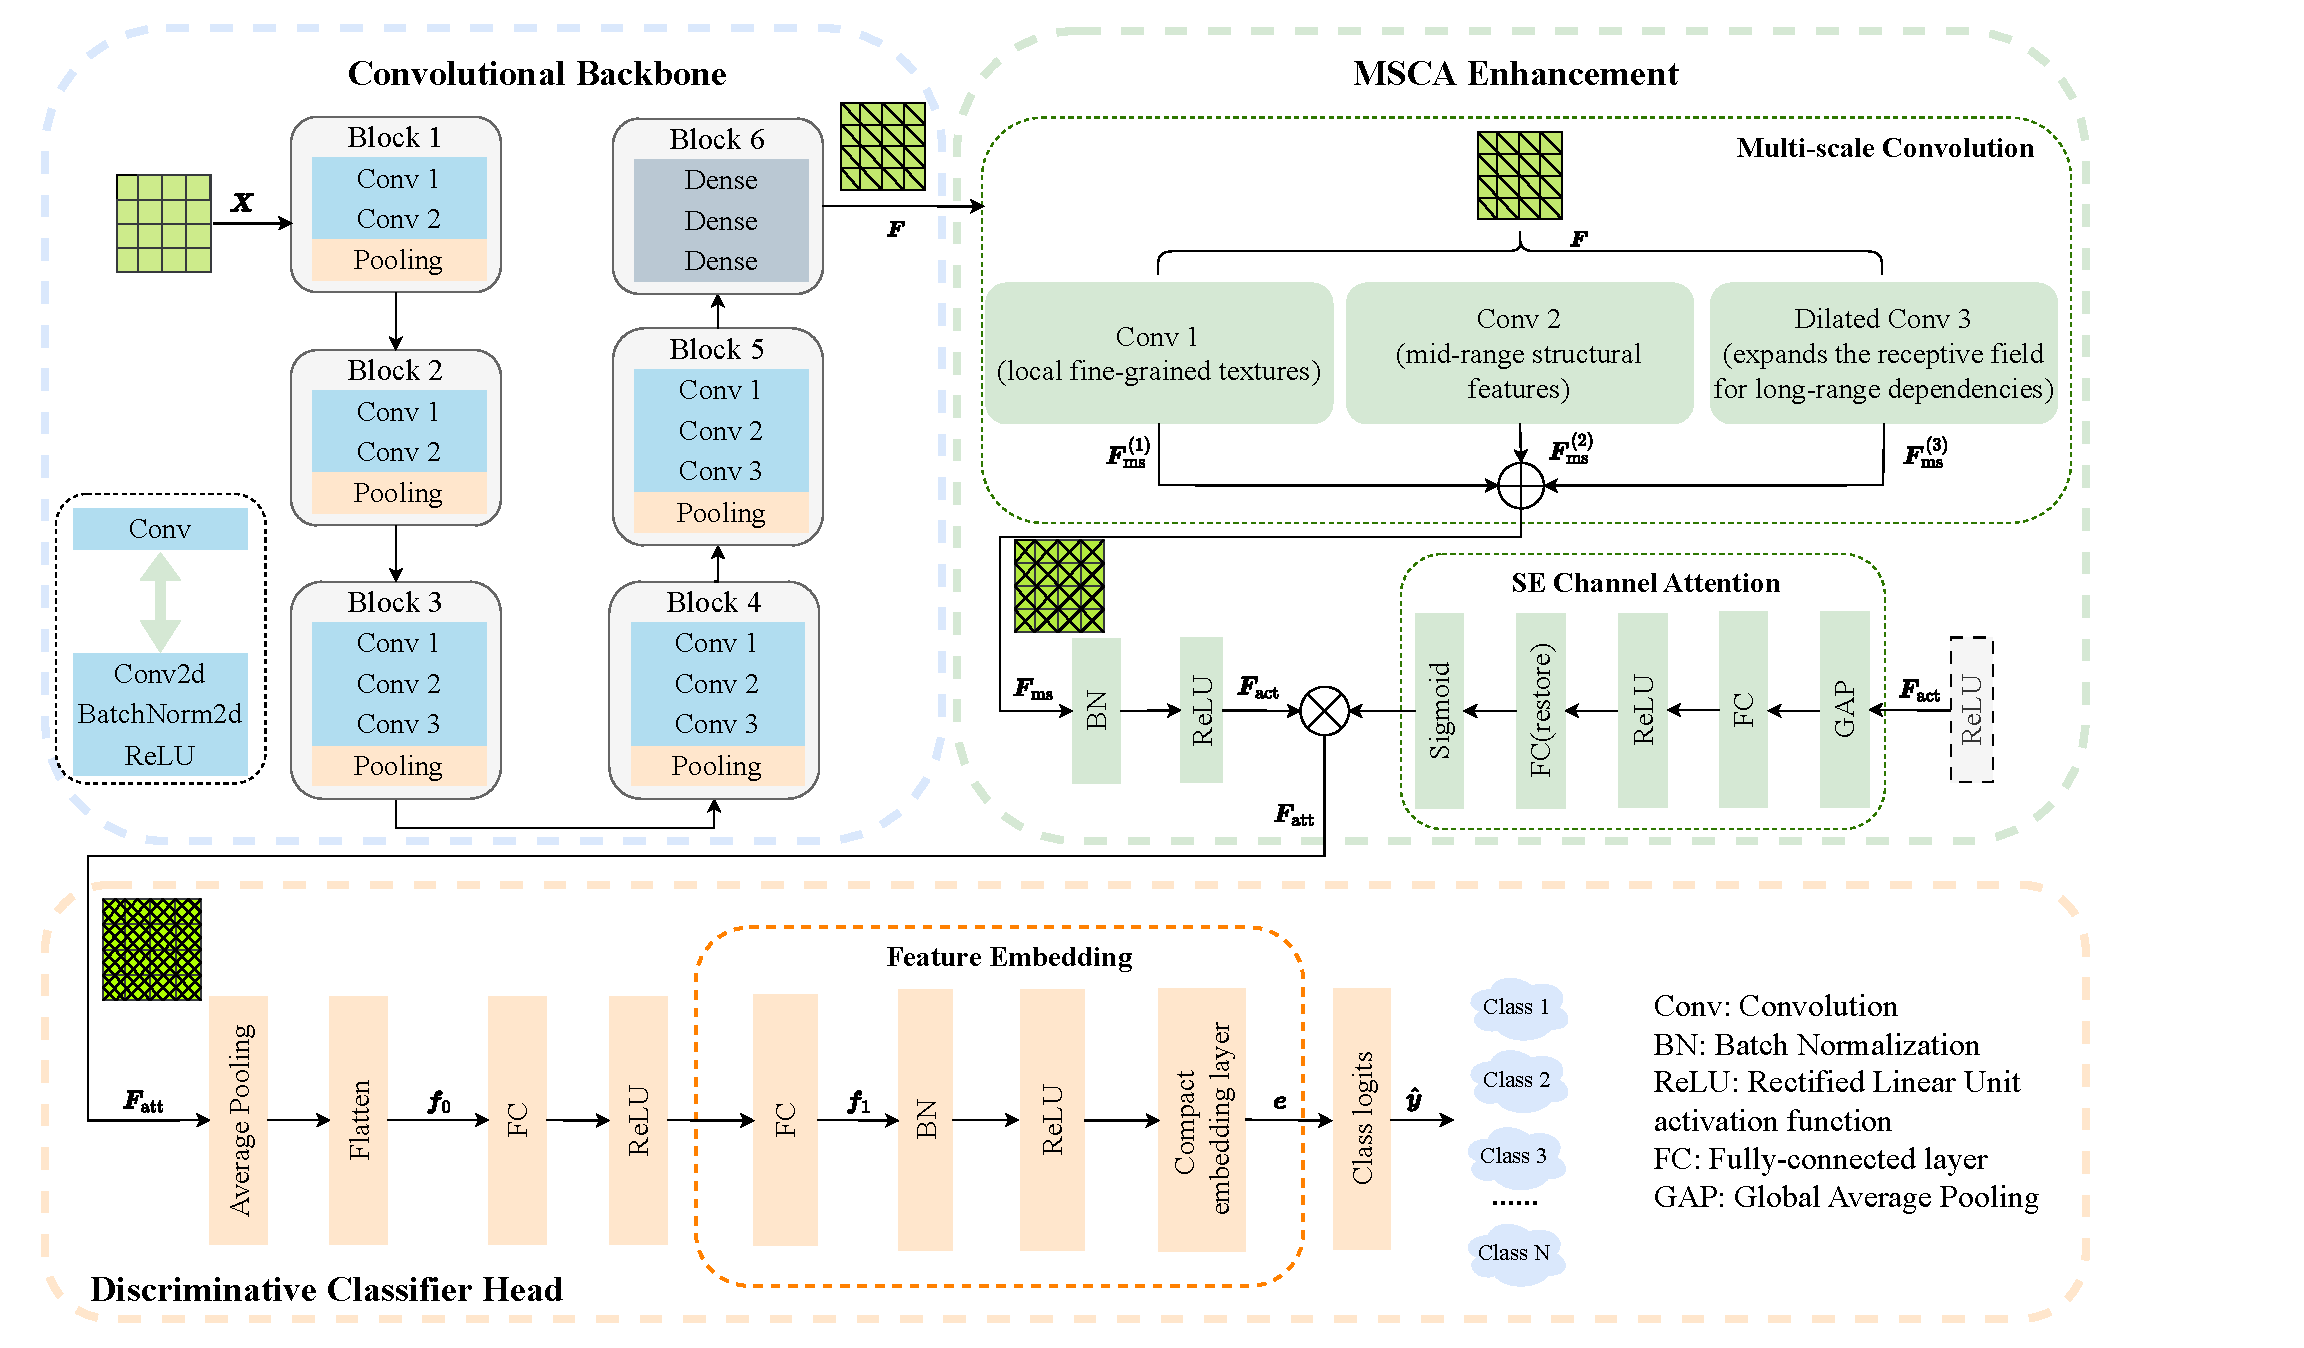
\includegraphics[width=\linewidth]{MSCA-VGG16/MSCA-VGG162.pdf}
\caption{Architecture of the proposed MSCA-VGG16 network. The fused AW-DPCNN image is processed by a VGG16-BN backbone, followed by multi-scale convolution (MS), squeeze-and-excitation channel attention (SE), and a compact embedding head (EH) for fault classification.}
\label{fig:msca_vgg16}
\end{figure*}

\subsection{MSCA-VGG16 for Fused Representation Classification}
\label{sec:msca_vgg16}

\subsubsection{Design Philosophy and Overview}

The AW-DPCNN fused representations contain heterogeneous features spanning multiple scales and frequency bands. To fully exploit this complementary information, we develop a Multi-Scale Channel Attention enhanced network (MSCA-VGG16) built upon three design principles: (i) \emph{multi-scale receptive field alignment} to capture fault patterns at different temporal and spectral granularities; (ii) \emph{dynamic channel recalibration} via squeeze-and-excitation to suppress noise-dominated frequency bands while amplifying fault-sensitive responses; and (iii) \emph{compact discriminative embedding} to project high-dimensional convolutional features into a lower-dimensional space for enhanced intra-class compactness and inter-class separability.

The overall architecture is a modular composition of a convolutional backbone $\mathcal{B}(\cdot)$, a multi-scale channel attention module $\mathcal{M}(\cdot)$, global pooling $\mathcal{P}(\cdot)$, an embedding projection $\mathcal{E}(\cdot)$, and a linear classifier $\mathcal{F}_{cls}(\cdot)$. The forward mapping from input $\boldsymbol{X}$ to predicted class probabilities $\hat{\mathbf{y}}$ is
\begin{equation}
\hat{\mathbf{y}} = \mathcal{F}_{cls}\big(\mathcal{E}\big(\mathcal{P}\big(\mathcal{M}\big(\mathcal{B}(\boldsymbol{X})\big)\big)\big)\big),
\label{eq:cls_pipeline}
\end{equation}
where $\boldsymbol{X} \in \mathbb{R}^{H_0 \times W_0 \times 3}$ denotes the AW-DPCNN fused pseudo-color image of spatial size $H_0 \times W_0$. The overall architecture is illustrated in Fig.~\ref{fig:msca_vgg16}. The following subsections detail each component.

\subsubsection{Convolutional Backbone}

VGG16 with batch normalization (VGG16-BN) is selected as the convolutional backbone. Its purely sequential topology without skip connections, built-in attention, or multi-scale processing provides a clean architectural baseline, ensuring that performance gains can be unambiguously attributed to the proposed MS, CA, and EH modules. The backbone maps the fused input image $\boldsymbol{X} \in \mathbb{R}^{H_0 \times W_0 \times 3}$ to a feature map
\begin{equation}
\boldsymbol{F} = \mathcal{B}(\boldsymbol{X}), \quad \boldsymbol{F} \in \mathbb{R}^{H \times W \times C},
\label{eq:feature_map}
\end{equation}
where $H$, $W$, and $C$ denote the spatial height, width, and number of channels, respectively. A comparative validation against alternative backbones is provided in Section~\ref{sec:backbone_comparison}.

\subsubsection{Multi-Scale Convolution Module}

Fault signatures in fused representations span multiple scales, from fine-grained local anomalies to long-range structural correlations. To align the network's receptive field with this multi-scale nature, we introduce a multi-scale convolution (MS) module comprising three parallel branches: a $3\times3$ convolution for local fine-grained textures, a $5\times5$ convolution for mid-range structural features, and a $3\times3$ dilated convolution with rate~2 that expands the receptive field without additional parameters for long-range dependencies. Each branch is formulated as

\begin{equation}
\begin{aligned}
\boldsymbol{F}_{\mathrm{ms}}^{(1)} &= \boldsymbol{\Theta}_{3} * \boldsymbol{F}, \\
\boldsymbol{F}_{\mathrm{ms}}^{(2)} &= \boldsymbol{\Theta}_{5} * \boldsymbol{F}, \\
\boldsymbol{F}_{\mathrm{ms}}^{(3)} &= \boldsymbol{\Theta}_{\mathrm{d}} * \boldsymbol{F},
\end{aligned}
\label{eq:multi_scale_branches}
\end{equation}

where $*$ denotes convolution, $\boldsymbol{\Theta}_{3},\boldsymbol{\Theta}_{5},\boldsymbol{\Theta}_{\mathrm{d}} \in \mathbb{R}^{C \times C \times k \times k}$ are learnable kernels with sizes $3\times3$, $5\times5$, and $3\times3$ (dilation~2), respectively. Each branch preserves the channel dimensionality $C$ through appropriate padding. The multi-scale features are fused via element-wise summation, which encourages each branch to specialize in complementary scales,

\begin{equation}
\boldsymbol{F}_{\mathrm{ms}} = \boldsymbol{F}_{\mathrm{ms}}^{(1)} + \boldsymbol{F}_{\mathrm{ms}}^{(2)} + \boldsymbol{F}_{\mathrm{ms}}^{(3)}.
\label{eq:multi_scale_fusion}
\end{equation}

The aggregated feature map is normalized and activated,
\begin{equation}
\boldsymbol{F}_{\mathrm{act}} = \delta\big(\mathrm{BN}(\boldsymbol{F}_{\mathrm{ms}})\big),
\label{eq:active_feature}
\end{equation}
where $\delta(\cdot) = \max(0, \cdot)$ is the ReLU activation and $\mathrm{BN}(\cdot)$ denotes batch normalization.

\subsubsection{Squeeze-and-Excitation Channel Attention}

Different frequency bands in the fused representation carry unequal diagnostic information. Some channels encode fault-critical spectral components, while others are dominated by background noise or redundant textures. To dynamically recalibrate channel-wise responses, we adopt a squeeze-and-excitation (SE) mechanism after the multi-scale fusion stage.

Let $\boldsymbol{F}_{\mathrm{act}} \in \mathbb{R}^{H \times W \times C}$ be the input to the SE module. The \emph{squeeze} operation aggregates spatial information into a channel descriptor $\boldsymbol{z} \in \mathbb{R}^{C}$ via global average pooling,
\begin{equation}
z_c = \frac{1}{H W} \sum_{i=1}^{H} \sum_{j=1}^{W} \boldsymbol{F}_{\mathrm{act}}(i, j, c), \quad c = 1, \dots, C.
\label{eq:se_squeeze}
\end{equation}

The \emph{excitation} operation models channel-wise dependencies through a bottleneck structure,
\begin{equation}
\boldsymbol{s} = \sigma\big(\boldsymbol{U}_2 \, \delta(\boldsymbol{U}_1 \boldsymbol{z})\big),
\label{eq:se_excitation}
\end{equation}
where $\boldsymbol{U}_1 \in \mathbb{R}^{\frac{C}{r} \times C}$ and $\boldsymbol{U}_2 \in \mathbb{R}^{C \times \frac{C}{r}}$ are learnable weight matrices, $r$ is the channel reduction ratio controlling the bottleneck capacity, and $\sigma(\cdot)$ is the sigmoid function. The output $\boldsymbol{s} = [s_1, \dots, s_C]^\top$ represents per-channel attention weights in $[0, 1]$. The refined feature map is obtained by channel-wise rescaling,

\begin{equation}
\boldsymbol{F}_{\mathrm{att}}(i, j, c) = s_c \cdot \boldsymbol{F}_{\mathrm{act}}(i, j, c).
\label{eq:attention_feature}
\end{equation}

This mechanism allows the network to emphasize channels containing fault-discriminative information while attenuating noise-dominated channels. The reduction ratio $r$ is specified in the experiment configuration.

\subsubsection{Compact Discriminative Embedding Head}

To promote intra-class compactness and inter-class separation while limiting parameter count, we replace conventional large fully-connected layers with a compact embedding head.

First, the spatially refined feature map $\boldsymbol{F}_{\mathrm{att}}$ is collapsed via global average pooling and flattened,

\begin{equation}
\boldsymbol{f}_0 = \mathrm{Flatten}\big(\mathrm{AvgPool}(\boldsymbol{F}_{\mathrm{att}})\big) \in \mathbb{R}^{C}.
\label{eq:flatten_feature}
\end{equation}

A fully-connected projection layer extracts high-level features,
\begin{equation}
\boldsymbol{f}_1 = \delta\big(\boldsymbol{W}_{\!fc1}\, \boldsymbol{f}_0\big), \quad \boldsymbol{W}_{\!fc1} \in \mathbb{R}^{D_1 \times C},
\label{eq:fc1_feature}
\end{equation}
followed by dropout for regularization. A compact embedding layer then projects $\boldsymbol{f}_1$ into a $d$-dimensional discriminative space,
\begin{equation}
\boldsymbol{e} = \delta\big(\mathrm{BN}(\boldsymbol{W}_{\!e}\, \boldsymbol{f}_1)\big), \quad \boldsymbol{e} \in \mathbb{R}^{d},
\label{eq:embedding}
\end{equation}
where $\boldsymbol{W}_{\!e} \in \mathbb{R}^{d \times D_1}$. Batch normalization is applied prior to ReLU to stabilize the feature distribution. Dropout is applied after each activation during training and disabled at inference. Finally, the class logits are obtained via a linear classifier,
\begin{equation}
\hat{\boldsymbol{y}} = \mathrm{softmax}(\boldsymbol{W}_{\!c}\, \boldsymbol{e}), \quad \boldsymbol{W}_{\!c} \in \mathbb{R}^{K \times d},
\label{eq:classifier}
\end{equation}
where $K$ is the number of fault categories. The dimensions $D_1$ (projection layer width) and $d$ (embedding dimensionality), as well as the dropout probability, are treated as hyperparameters whose concrete values are given in Section~\ref{section4}. The entire network is optimized by minimizing the cross-entropy loss,
\begin{equation}
\mathcal{L}_{\mathrm{CE}} = -\sum_{k=1}^{K} y_k \log \hat{y}_k,
\label{eq:cross_entropy_loss}
\end{equation}
where $\boldsymbol{y} = [y_1, \dots, y_K]^\top$ is the one-hot ground-truth label. In practice, a class-weighted variant $\mathcal{L}_{\mathrm{wCE}}$ is employed to counteract dataset imbalance (Section~\ref{section4}).

\subsubsection{Forward Pass Algorithm}

Algorithm~\ref{alg:msca_vgg16} summarizes the complete forward pass of the proposed MSCA-VGG16 network from the fused input image to the predicted class probabilities.

\begin{algorithm}
\caption{Forward Pass of MSCA-VGG16}
\label{alg:msca_vgg16}
\begin{algorithmic}[1]
\Require Fused AW-DPCNN image $\boldsymbol{X} \in \mathbb{R}^{H_0 \times W_0 \times 3}$
\State Extract backbone feature map $\boldsymbol{F}$ using Eq.~\ref{eq:feature_map}.
\State Compute multi-scale feature $\boldsymbol{F}_{\mathrm{ms}}$ using Eq.~\ref{eq:multi_scale_fusion}.
\State Apply BatchNorm and ReLU to obtain $\boldsymbol{F}_{\mathrm{act}}$ using Eq.~\ref{eq:active_feature}.
\State Squeeze spatial information into channel descriptor $\boldsymbol{z}$ using Eq.~\ref{eq:se_squeeze}.
\State Compute channel attention weights $\boldsymbol{s}$ using Eq.~\ref{eq:se_excitation}.
\State Obtain channel-refined feature $\boldsymbol{F}_{\mathrm{att}}$ using Eq.~\ref{eq:attention_feature}.
\State Apply global average pooling and flatten to obtain $\boldsymbol{f}_0$ using Eq.~\ref{eq:flatten_feature}.
\State Project to high-level features $\boldsymbol{f}_1$ using Eq.~\ref{eq:fc1_feature}, then apply dropout.
\State Compute compact embedding $\boldsymbol{e}$ using Eq.~\ref{eq:embedding}, then apply dropout.
\State Produce class probabilities $\hat{\boldsymbol{y}}$ using Eq.~\ref{eq:classifier}.
\Ensure Predicted class probabilities $\hat{\boldsymbol{y}} \in \mathbb{R}^{K}$.
\end{algorithmic}
\end{algorithm}

\section{Dataset and Experiments}

\label{section4}
\subsection{Dataset Construction and Preprocessing}
\label{Dataset Construction and Preprocessing}

The Case Western Reserve University (CWRU) bearing dataset is employed as the primary benchmark for evaluating the proposed method. The experimental test stand, shown in Fig.~\ref{fig:cwru_teststand}, consists of a 2-hp motor, a torque transducer/encoder, a dynamometer, and control electronics. Vibration data were collected using accelerometers mounted at both the drive-end (DE) and fan-end (FE) of the motor housing, at sampling rates of 12~kHz and 48~kHz.

\begin{figure}[!t]
	\centering
	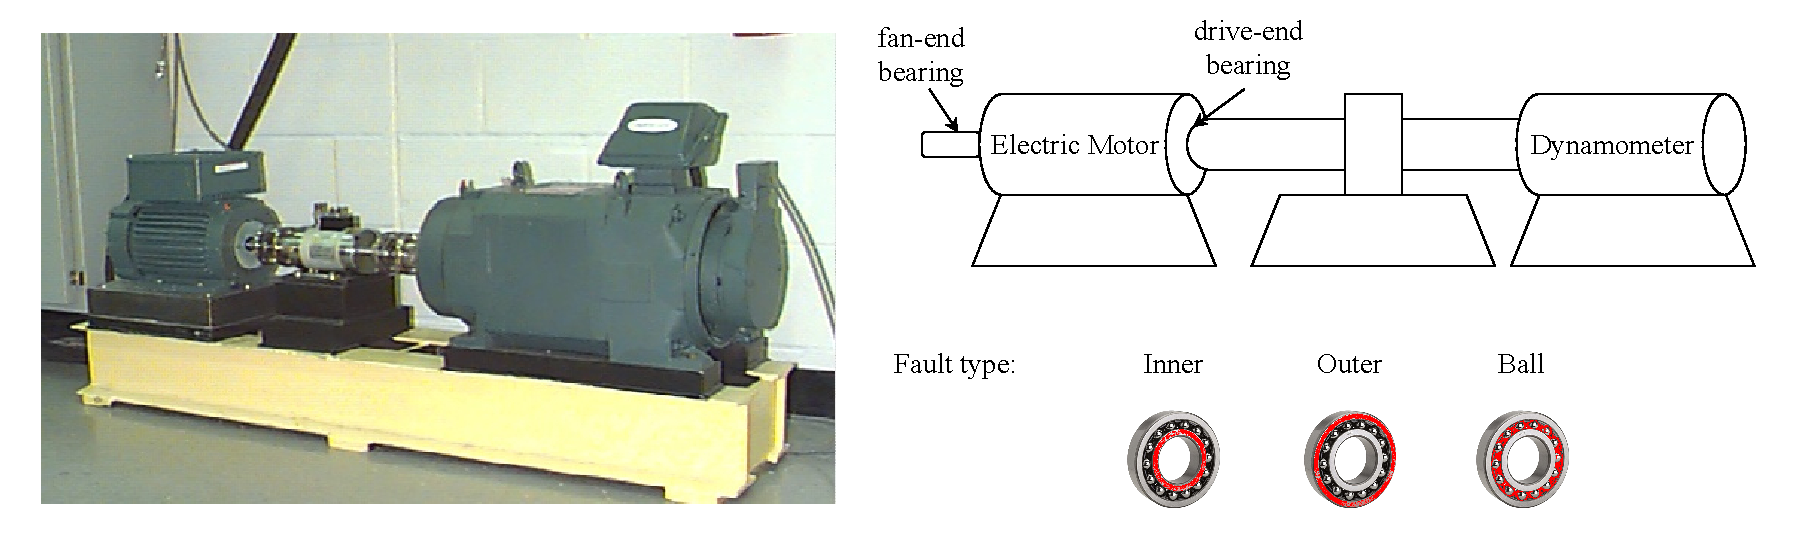
\includegraphics[width=\linewidth]{equipment/cwru1 }
	\caption{CWRU bearing test stand. Vibration signals were collected from accelerometers at the drive-end and fan-end positions under four operating loads (0--3 hp).}
	\label{fig:cwru_teststand}
\end{figure}

Single-point faults of diameters 0.007, 0.014, and 0.021 inches were separately introduced to the ball, inner race, and outer race (at the 6 o'clock load zone position) using electro-discharge machining. Together with the healthy baseline condition, this yields ten categories as listed in Table~\ref{tab:operating_conditions}. Each fault class contains four source recordings of approximately 10~seconds duration; the normal baseline recordings are approximately 40~seconds long.

For dataset construction, the raw vibration signals are segmented into overlapping windows and converted into pseudo-color fused images through the AW-DPCNN pipeline. Three dataset variants are constructed to support comprehensive evaluation:

\begin{enumerate}
\item \textbf{CWRU 12k DE (primary benchmark):} 12~kHz drive-end signals with window length 2048 samples (170.7~ms) and hop length 1024 samples (85.3~ms). FFT window size $N_{\text{FFT}}=1024$, yielding 11.7~Hz/bin frequency resolution. Maximum frequency $f_{\max}=6$~kHz (full Nyquist bandwidth at 12~kHz sampling).
\item \textbf{CWRU 12k FE (cross-sensor generalization):} 12~kHz fan-end signals with identical time--frequency parameters to the 12k DE dataset, enabling evaluation of sensor-position transferability.
\item \textbf{CWRU 48k DE (cross-sampling-rate generalization):} 48~kHz drive-end signals with window length 8192 samples (170.7~ms) and hop length 4096 samples (85.3~ms). FFT window size $N_{\text{FFT}}=4096$, maintaining identical temporal duration and frequency resolution (11.7~Hz/bin). Maximum frequency extended to $f_{\max}=24$~kHz to exploit the richer high-frequency information at the higher sampling rate.
\end{enumerate}

The window and hop lengths are scaled proportionally with the sampling rate to ensure that every fused image represents the same physical duration (170.7~ms) of vibration signal, eliminating temporal-scale confounds from cross-dataset comparisons. File-level stratified splitting is applied with a 60\%/20\%/20\% (train/validation/test) ratio, using a fixed random seed (42) for reproducibility. All windows from a given source recording are assigned exclusively to a single split to prevent data leakage. The detailed dataset composition, including sample counts per class and per split, is provided in Table~\ref{tab:datasets_comprehensive} (presented later in this section).

For the primary benchmark (12k DE), the normal class contains substantially more windows than fault classes (708 train / 473 validation / 471 test vs.\ approximately 235 / 117 / 118 per fault class) because the normal baseline recordings are approximately four times longer. This inherent class imbalance is addressed through class-weighted cross-entropy loss and macro-averaged evaluation metrics. All datasets use the linear STFT spectrogram as the time--frequency representation and GADF as the temporal encoding, with the optimal combination validated through systematic representation comparison experiments in Section~\ref{sec:rep_compare}.


\begin{table}[!t]
	\caption{CWRU Bearing Dataset: Operating Conditions and Corresponding Labels}
	\centering
	\begin{tabular}{ll}
		\toprule
		Label & Description \\
		\midrule
		Normal & Healthy Baseline \\
		BF007 & Ball Fault (0.007'') \\
		BF014 & Ball Fault (0.014'') \\
		BF021 & Ball Fault (0.021'') \\
		IF007 & Inner Race Fault (0.007'') \\
		IF014 & Inner Race Fault (0.014'') \\
		IF021 & Inner Race Fault (0.021'') \\
		OF007 & Outer Race Fault @6 (0.007'') \\
		OF014 & Outer Race Fault @6 (0.014'') \\
		OF021 & Outer Race Fault @6 (0.021'') \\
		
		\bottomrule
	\end{tabular}
	\label{tab:operating_conditions}
\end{table}


\begin{table}[!t]
\centering
\caption{Class-wise sample distribution of three CWRU bearing datasets (60/20/20 train/val/test split, seed 42). All datasets: $T_{\text{win}}=170.7$\,ms, $\Delta f=11.7$\,Hz/bin, Jensen--Shannon $D_{\text{JS}} \leq 0.064$. BF: Ball Fault; IF: Inner Race Fault; OF: Outer Race Fault @6$'$. Fault diameters: 007, 014, 021\,mil.}
\label{tab:datasets_comprehensive}
\small
\renewcommand{\arraystretch}{1.0}
\setlength{\tabcolsep}{5pt}
\begin{tabular}{lcccc}
\toprule
\textbf{Dataset} & \textbf{Class} & \textbf{Train} & \textbf{Val} & \textbf{Test} \\
\midrule
\multirow{11}{*}{\textbf{CWRU 12k DE}} 
& BF007  & 234 & 117 & 118 \\
& BF014  & 236 & 117 & 118 \\
& BF021  & 235 & 118 & 118 \\
& IF007  & 236 & 117 & 119 \\
& IF014  & 234 & 117 & 117 \\
& IF021  & 235 & 117 & 118 \\
& OF007  & 236 & 118 & 117 \\
& OF014  & 234 & 118 & 118 \\
& OF021  & 236 & 118 & 118 \\
& Normal & 708 & 473 & 471 \\
& \textbf{Total} & \textbf{2824} & \textbf{1530} & \textbf{1532} \\
\midrule
\multirow{11}{*}{\textbf{CWRU 12k FE}} 
& BF007  & 233 & 117 & 117 \\
& BF014  & 235 & 118 & 117 \\
& BF021  & 233 & 117 & 117 \\
& IF007  & 234 & 117 & 117 \\
& IF014  & 234 & 117 & 117 \\
& IF021  & 234 & 117 & 117 \\
& OF007  & 235 & 117 & 117 \\
& OF014  & 69  & 22  & 22  \\
& OF021  & 69  & 22  & 22  \\
& Normal & 708 & 473 & 471 \\
& \textbf{Total} & \textbf{2484} & \textbf{1337} & \textbf{1334} \\
\midrule
\multirow{11}{*}{\textbf{CWRU 48k DE}} 
& BF007  & 234 & 118 & 58  \\
& BF014  & 234 & 59  & 117 \\
& BF021  & 234 & 117 & 58  \\
& IF007  & 234 & 58  & 117 \\
& IF014  & 236 & 117 & 14  \\
& IF021  & 235 & 118 & 58  \\
& OF007  & 235 & 58  & 117 \\
& OF014  & 175 & 117 & 118 \\
& OF021  & 236 & 59  & 118 \\
& Normal & 175 & 117 & 117 \\
& \textbf{Total} & \textbf{2228} & \textbf{938}  & \textbf{892}  \\
\bottomrule
\end{tabular}
\end{table}


% \begin{table*}
% 	\centering
% 	\caption{Composition of the CWRU Bearing Dataset (12 kHz Drive‑End)}
% 	\label{dataset}
% 	\renewcommand{\arraystretch}{1.15}
% 	\small
% 	\begin{tabular}{l c c c c c c c c c c c}
% 		\toprule
% 		\multirow{2}{*}{Split} &
% 		\multirow{2}{*}{Total} &
% 		\multicolumn{10}{c}{Number of Samples per Class} \\
% 		\cmidrule(lr){3-12}
% 		& & BF007 & BF014 & BF021 & IF007 & IF014 & IF021 & OF007 & OF014 & OF021 & Normal \\
% 		\midrule
% 		Source files & 40 & 4 & 4 & 4 & 4 & 4 & 4 & 4 & 4 & 4 & 4 \\
% 		\midrule
% 		Training set  & 1397 & 116 & 116 & 116 & 116 & 116 & 116 & 116 & 116 & 116 & 353 \\
% 		Validating set & 758 & 58 & 58 & 58 & 58 & 58 & 58 & 58 & 58 & 58 & 236 \\
% 		Testing set   & 758 & 58 & 58 & 58 & 59 & 58 & 58 & 58 & 58 & 58 & 235 \\
% 		\bottomrule
% 	\end{tabular}
% \end{table*}






As shown in Table~\ref{dataset}, each fault class consists of 4 source recordings, which are partitioned into training, validation, and test subsets at a ratio of approximately 2:1:1 at the file level. The Normal baseline condition contains substantially more windows than the fault categories because the normal-operation recordings in the CWRU dataset are approximately $4\times$ longer than the fault recordings (roughly 40~s versus 10~s per recording). This inherent class imbalance reflects the physical ground truth of the data acquisition protocol and is addressed through two complementary strategies: a class-weighted cross-entropy loss during training to prevent the model from being biased toward the majority class, and macro-averaged evaluation metrics to ensure that each class contributes equally to the reported performance regardless of sample count.

Fig.~\ref{Fig: Fused images} illustrates the representations of different bearing conditions before and after adaptive fusion. The STFT spectrogram primarily reflects frequency-domain energy distributions, where different fault types exhibit distinct spectral patterns corresponding to their characteristic fault frequencies. In contrast, GADF images encode temporal correlations and periodic structures of the vibration signals, revealing complementary information that is not explicitly captured in the time--frequency domain.
\begin{figure*}[!t]
	\centering
	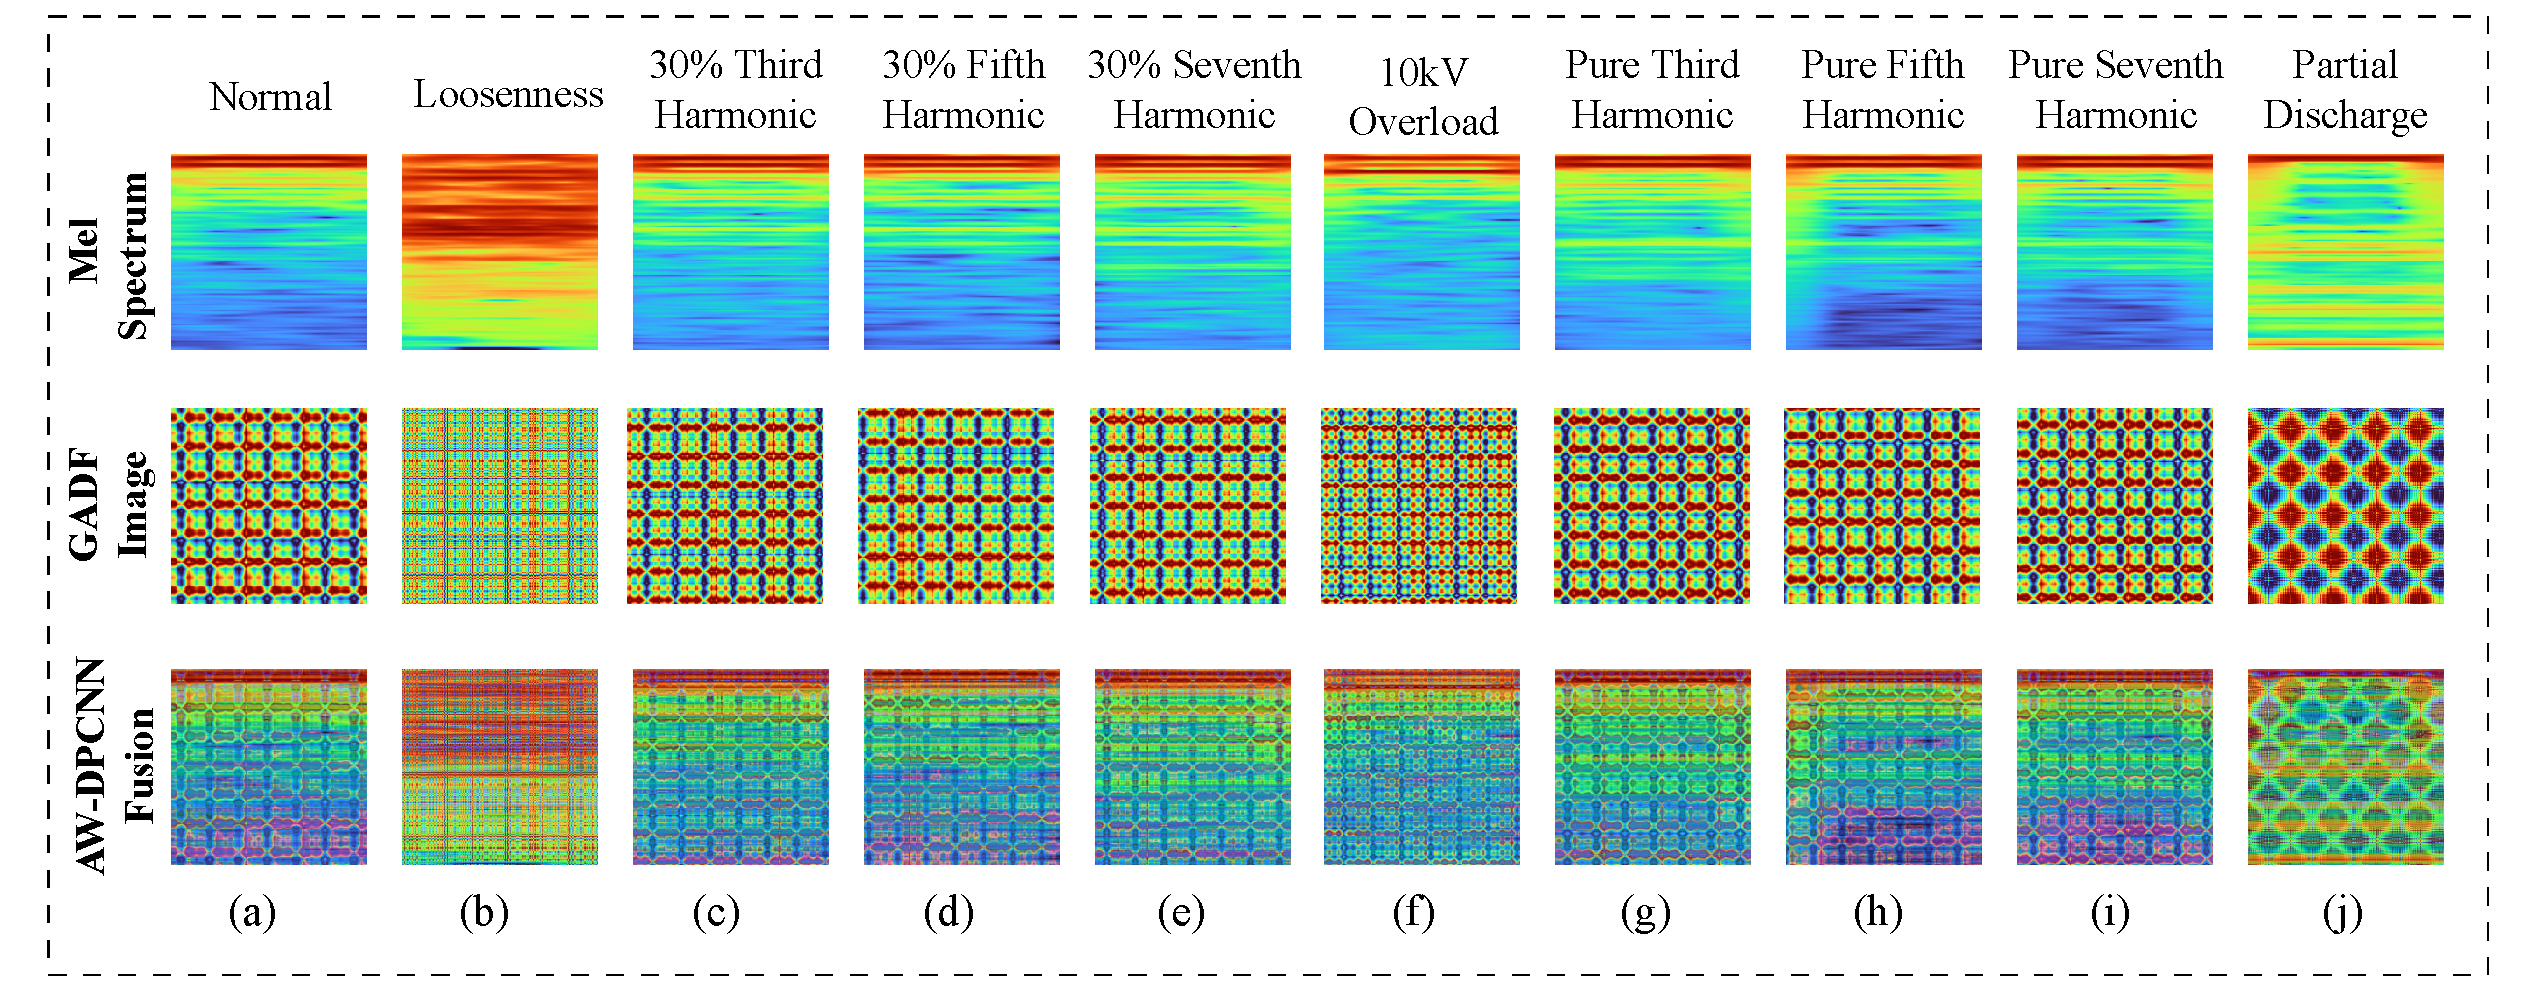
\includegraphics[width=\textwidth]{Fused images/Fused images}
	\caption{Visualization of STFT spectrograms, GADF images, and adaptively fused representations generated by the proposed AW-DPCNN under different bearing conditions. (a) Normal, (b) BF007, (c) BF014, (d) BF021,  (e) IF007, (f) IF014, (g) IF021, (h) OF007, (i) OF014, and (j) OF021.}
	\label{Fig: Fused images}
\end{figure*}


After processing by the proposed AW-DPCNN, the fused feature maps exhibit enhanced structural clarity and improved discrimination among different fault types. Notably, background noise and redundant patterns are effectively suppressed, while salient fault-related features are preserved and highlighted. This qualitative analysis demonstrates that the AW-DPCNN is capable of adaptively integrating frequency-domain and temporal-domain information, thereby generating more informative representations for subsequent fault classification.

\subsection{Implementation Details and Evaluation Metrics}
The raw vibration signals are converted into STFT spectrograms and GADF images, which are subsequently fused using the proposed AW-DPCNN to generate pseudo-color RGB images of size $224 \times 224$. These fused representations serve as the input to the MSCA-VGG16 network. All experiments follow a unified training protocol. During each ablation study, only one factor is modified while all other settings remain unchanged.

To mitigate the adverse effects of class imbalance inherent in the CWRU bearing dataset, a class-weighted cross-entropy loss is adopted. Specifically, the weight $w_k$ for class $k$ is computed as
\begin{equation}
w_k = \frac{N_{\mathrm{total}}}{K \cdot N_k},
\label{eq:class_weight}
\end{equation}
where $N_{\mathrm{total}}$ denotes the total number of training samples, $K$ is the number of fault categories, and $N_k$ is the number of training samples belonging to class $k$. The weighted cross-entropy loss is then formulated as
\begin{equation}
\mathcal{L}_{\mathrm{wCE}} = -\frac{1}{B} \sum_{i=1}^{B} w_{y_i} \sum_{k=1}^{K} \boldsymbol{y}_{i,k} \log \hat{\boldsymbol{y}}_{i,k},
\label{eq:weighted_ce}
\end{equation}
where $w_{y_i}$ is the class weight of the ground-truth label, $\boldsymbol{y}_{i,k}$ is the $k$-th entry of the one-hot encoded label vector, and $\hat{\boldsymbol{y}}_{i,k}$ is the predicted probability for class $k$. This weighting strategy ensures that minority classes receive proportionally larger loss contributions, preventing the model from being biased toward majority classes.

All models are optimized using AdamW with an initial learning rate $\eta=1\times10^{-4}$ and weight decay $\lambda=1\times10^{-3}$. A ReduceLROnPlateau scheduler reduces the learning rate by a factor of $0.5$ when the validation F1-score does not improve for 5 consecutive epochs, down to a minimum of $\eta_{\min}=1\times10^{-6}$. Training uses a batch size of $B=32$ for up to $E_{\max}=30$ epochs. Data augmentation consists of random horizontal flipping ($p_{\mathrm{flip}}=0.5$) and random rotation within $\pm10^\circ$. Input images are normalized using ImageNet statistics, which aligns with the pretrained VGG16-BN backbone. Early stopping is triggered if the validation macro-averaged F1-score does not improve for $p_{\mathrm{es}}=15$ consecutive epochs, and the model checkpoint with the highest validation F1-score is retained for final evaluation on the held-out test set.

To ensure statistical reliability and to account for performance variance due to random initialization, all key experiments are repeated over three independent trials with different random seeds (42, 123, 456). The aggregated results are reported as mean $\pm$ standard deviation across the three trials.

The experiments in this study were conducted on a system equipped with an Intel i9-14900K CPU and an NVIDIA RTX 5090 GPU. The software environment was based on PyTorch 2.11 and CUDA 12.8. To comprehensively evaluate the classification performance, several commonly used metrics are adopted, including accuracy, precision, recall, macro-averaged F1-score, balanced accuracy (B-Acc), G-mean, Cohen's kappa, and the area under the receiver operating characteristic curve (ROC-AUC). For multi-class ROC-AUC, the One-vs-Rest (OvR) strategy is employed and the macro-averaged AUC is reported, ensuring balanced assessment across all fault categories regardless of class imbalance.

	\begin{figure*}[!htbp]
		\centering
		\begin{subfigure}{0.42\textwidth}
			\centering
			\includegraphics[width=\linewidth]{confusion_matrix_48k_de_convnext_tiny_exp1_convnext_tiny_trial_seed123}
			\caption{convnext Tiny}
		\end{subfigure}
		\hfill
		\begin{subfigure}{0.42\textwidth}
			\centering
			\includegraphics[width=\linewidth]{confusion_matrix_48k_de_efficientnet_b0_exp1_efficientnet_b0_trial_seed456}
			\caption{efficientnet B0}
		\end{subfigure}\\[2mm]

		\begin{subfigure}{0.42\textwidth}
			\centering
			\includegraphics[width=\linewidth]{confusion_matrix_48k_de_vit_exp1_vit_trial_seed42}
			\caption{Vit}
		\end{subfigure}
		\hfill
		\begin{subfigure}{0.42\textwidth}
			\centering
			\includegraphics[width=\linewidth]{confusion_matrix_48k_de_mobilenetv3_small_exp1_mobilenetv3_small_trial_seed42}
			\caption{MobileNetV3-Small}
		\end{subfigure}\\[2mm]

		\begin{subfigure}{0.42\textwidth}
			\centering
			\includegraphics[width=\linewidth]{confusion_matrix_48k_de_vgg16_exp1_vgg16_trial_seed123}
			\caption{VGG16}
		\end{subfigure}
		\hfill
		\begin{subfigure}{0.42\textwidth}
			\centering
			\includegraphics[width=\linewidth]{confusion_matrix_12k_de_MSCA_VGG16_exp1_MSCA_VGG16_trial_seed123}
			\caption{MSCA-VGG16 (Ours)}
		\end{subfigure}
		\caption{Confusion matrices of different network backbones trained using the AW-DPCNN fusion representations. The proposed MSCA-VGG16 achieves the most accurate classification performance with significantly reduced inter-class confusion.}
		\label{fig:confusion_matrix}
	\end{figure*}





\subsection{Representation Comparison}
\label{sec:rep_compare}

The proposed AW-DPCNN framework adopts the STFT spectrogram as the time--frequency representation and the GADF as the temporal encoding method. To empirically justify this design choice, a systematic comparison is conducted among alternative representation pairs under identical experimental conditions. Specifically, three time--frequency representations (STFT spectrogram, Mel spectrogram, and Morlet CWT scalogram) and four temporal encoding methods (GADF, GASF, Markov Transition Field (MTF), and Recurrence Plot (RP)) are evaluated, resulting in twelve representation combinations. All representations are fused through the same AW-DPCNN pipeline ($\gamma=10$, $N=20$) and classified using the identical MSCA-VGG16 network, thereby isolating the effect of the input representation on diagnostic performance.

The dataset construction follows the procedure described in Section~\ref{Dataset Construction and Preprocessing}. For each combination, the raw vibration signals are converted into the corresponding time--frequency and temporal representations, fused via AW-DPCNN into pseudo-color images of size $224\times 224$, and subsequently fed into the MSCA-VGG16 classifier. All training hyperparameters are kept consistent across runs.

% Auto-generated by scripts/analyze_results.py
% Date: 2026-06-30 17:37:58
% These tables can be \input{} directly into tim.tex
% ── Representation Comparison Table ──
\begin{table*}
    \centering
    \caption{Representation Comparison Across Time--Frequency and Temporal Encoding Methods. All combinations are fused via AW-DPCNN and classified by standard VGG16 network trained from scratch. Best values per metric are bolded.}
    \label{tab:rep_compare}
    \renewcommand{\arraystretch}{1.15}
    \small
    \begin{tabular}{llcccc}
        \toprule
        \textbf{TF Method} & \textbf{Temporal} & \textbf{Acc (\%)} & \textbf{F1 (\%)} & \textbf{G-mean (\%)} & \textbf{AUC (\%)} \\
        \midrule
        \multirow{4}{*}{Mel} & GADF & $89.18 \pm 1.87$ & $83.94 \pm 3.64$ & $77.27 \pm 6.99$ & $99.46 \pm 0.23$ \\
         & GASF & $93.53 \pm 2.22$ & $90.52 \pm 4.02$ & $86.27 \pm 8.92$ & $99.44 \pm 0.43$ \\
         & MTF & $94.08 \pm 1.08$ & $90.94 \pm 2.08$ & $86.27 \pm 4.76$ & $99.62 \pm 0.17$ \\
         & RP & $94.56 \pm 3.61$ & $92.55 \pm 4.96$ & $90.93 \pm 6.56$ & $99.57 \pm 0.36$ \\
        \cmidrule(lr){2-6}
        \multirow{4}{*}{STFT} & GADF & $\mathbf{96.30 \pm 0.49}$ & $\mathbf{95.02 \pm 0.40}$ & $\mathbf{94.22 \pm 0.49}$ & $\mathbf{99.97 \pm 0.03}$ \\
         & GASF & $91.23 \pm 0.65$ & $85.86 \pm 0.79$ & $69.32 \pm 8.26$ & $99.38 \pm 0.27$ \\
         & MTF & $90.16 \pm 7.46$ & $86.48 \pm 9.50$ & $78.92 \pm 17.99$ & $98.16 \pm 2.81$ \\
         & RP & $90.12 \pm 0.95$ & $84.28 \pm 0.95$ & $39.34 \pm 26.45$ & $99.35 \pm 0.04$ \\
        \cmidrule(lr){2-6}
        \multirow{4}{*}{CWT} & GADF & $89.70 \pm 1.53$ & $84.32 \pm 2.55$ & $76.01 \pm 6.93$ & $99.33 \pm 0.16$ \\
         & GASF & $89.81 \pm 1.30$ & $85.75 \pm 2.14$ & $80.87 \pm 3.91$ & $99.14 \pm 0.17$ \\
         & MTF & $90.01 \pm 2.72$ & $85.24 \pm 4.42$ & $77.00 \pm 9.29$ & $99.16 \pm 0.50$ \\
         & RP & $90.88 \pm 0.04$ & $87.43 \pm 0.39$ & $83.95 \pm 1.41$ & $98.99 \pm 0.13$ \\
        \bottomrule
    \end{tabular}
\end{table*}

Table~\ref{tab:rep_compare} reports the test-set performance of all twelve combinations. Several important observations emerge:

\textbf{1) Time--frequency representation comparison.} Among the three time--frequency methods, the STFT spectrogram consistently achieves the highest accuracy when paired with GADF (96.30\%), substantially outperforming the best Mel-based combination (Mel+RP, 94.56\%) and the best CWT-based combination (CWT+RP, 90.88\%). The uniform frequency resolution of the linear STFT spectrogram preserves fine-grained high-frequency fault signatures that are essential for distinguishing between different bearing fault severities, whereas the Mel-scale's nonlinear frequency compression and the CWT's variable resolution may obscure these discriminative spectral details.

\textbf{2) Temporal encoding comparison.} Among the four temporal encoding methods, GADF achieves the best performance when paired with STFT (96.30\%), significantly outperforming GASF (91.23\%), MTF (90.16\%), and RP (90.12\%). The GADF's angular difference encoding captures more discriminative temporal transition patterns than the summation-based GASF, and the structured correlation matrix provides richer information than the quantized transition probabilities of MTF or the binary recurrence patterns of RP. Notably, GADF paired with STFT achieves a G-mean of 94.22\%, far exceeding the next best combination (Mel+RP, 90.93\%), confirming that the STFT+GADF pair provides the most balanced class-wise discrimination.

\textbf{3) Optimal combination.} The STFT spectrogram paired with GADF achieves the best overall performance across all metrics, with 96.30\% accuracy, 95.02\% F1-score, and 94.22\% G-mean. This result empirically validates the choice of STFT+GADF as the input representation pair for the proposed AW-DPCNN framework. The STFT spectrogram provides uniform-resolution time--frequency energy distributions, while the GADF encodes complementary temporal correlation structures through angular differences, forming a jointly discriminative basis for bearing fault diagnosis. The representation comparison also reveals that some non-optimal pairs (e.g., Mel+RP at 94.56\%) can achieve competitive accuracy, suggesting that the AW-DPCNN fusion mechanism is sufficiently robust to extract discriminative features from suboptimal input representations, though the optimal STFT+GADF pair provides the best performance with the lowest variance.

These results collectively demonstrate that the STFT and GADF combination provides the most effective input representation for the AW-DPCNN fusion framework, offering consistent advantages over alternative time--frequency and temporal encoding methods. The empirical evidence supports the representation design adopted in this work and further validates the robustness of the proposed diagnostic pipeline.


% Auto-generated by scripts/analyze_results.py
% Date: 2026-06-30 17:37:58
% These tables can be \input{} directly into tim.tex
% ── Backbone Comparison Table ──
\begin{table*}
    \caption{Performance Comparison with Different Backbone Networks\label{tab:network_comparison}}
    \centering
    \renewcommand{\arraystretch}{1.15}
    \begin{tabular}{lcccccc}
        \toprule
        \textbf{Network} & \textbf{Acc (\%)} & \textbf{Recall (\%)} & \textbf{F1 (\%)} & \textbf{G-mean (\%)} & \textbf{B-Acc (\%)} & \textbf{Kappa (\%)} \\
        \midrule
        % \textbf{MSCA-VGG16 (Ours)} & $\mathbf{99.85 \pm 0.10}$ & $\mathbf{99.80 \pm 0.13}$ & $\mathbf{99.80 \pm 0.13}$ & $\mathbf{99.80 \pm 0.13}$ & $\mathbf{99.80 \pm 0.13}$ & $\mathbf{99.82 \pm 0.12}$ \\
        % \textbf{MSCA-VGG16 (Ours)} & $\mathbf{99.85 \pm 0.10}$ & $\mathbf{99.80 \pm 0.13}$ & $\mathbf{99.80 \pm 0.13}$ & $\mathbf{99.80 \pm 0.13}$ & $\mathbf{99.80 \pm 0.13}$ & $\mathbf{99.82 \pm 0.12}$ \\
        \textbf{MSCA-VGG16 (Ours)} & $\mathbf{99.85 \pm 0.10}$ & $\mathbf{99.84 \pm 0.22}$ & $\mathbf{99.46 \pm 0.43}$ & $\mathbf{99.82 \pm 0.15}$ & $\mathbf{99.86 \pm 0.13}$ & $\mathbf{99.82 \pm 0.12}$ \\
        VGG16 (Peng et al.\cite{9440949}) & $99.19 \pm 0.89$ & $98.95 \pm 1.16$ & $98.95 \pm 1.16$ & $98.91 \pm 1.22$ & $98.95 \pm 1.16$ & $99.06 \pm 1.05$ \\
        EfficientNet-B0 (Cheng et al.\cite{11028059})& $95.74 \pm 2.07$ & $94.47 \pm 2.68$ & $94.14 \pm 3.05$ & $93.08 \pm 4.09$ & $94.47 \pm 2.68$ & $95.00 \pm 2.43$ \\
        ViT (Liu et al.\cite{10663388}) & $82.35 \pm 0.89$ & $77.20 \pm 1.06$ & $74.71 \pm 2.19$ & $64.72 \pm 7.53$ & $77.20 \pm 1.06$ & $79.30 \pm 1.04$ \\
        MobileNetV3-Small (Zhang et al.\cite{ZHANG2026106301})& $93.69 \pm 1.64$ & $91.81 \pm 2.13$ & $91.03 \pm 2.69$ & $87.82 \pm 5.30$ & $91.81 \pm 2.13$ & $92.60 \pm 1.92$ \\
        ResNet18 (Duan et al.\cite{DUAN2026122469})& $ 98.39\pm 1.32$ & $97.91 \pm 1.71$ & $97.85 \pm1.81 $ & $ 97.66 \pm 2.10$ & $ 97.91\pm 1.71$ & $ 98.11\pm 1.55$ \\
        ConvNeXt-Tiny (Tu et al.\cite{10929672})& $92.93 \pm 2.12$ & $90.82 \pm 2.76$ & $90.63 \pm 2.50$ & $88.99 \pm 3.11$ & $90.82 \pm 2.76$ & $91.70 \pm 2.49$ \\
        \midrule
        VGG16 (STFT only\cite{9440949}) & $93.37\pm 1.32$ & $92.71 \pm1.45 $ & $91.49 \pm 2.25$ & $86.89\pm 5.47$ & $ 92.71\pm1.45 $ & $92.58\pm 1.48$ \\
        VGG16 (GADF only\cite{9440949}) & $60.99\pm 1.50$ & $ 62.71\pm 2.51$ & $ 56.90\pm 2.13$ & $ 12.93\pm 1.42$ & $ 62.71\pm 2.51$ & $ 56.75\pm 1.37$ \\
        \bottomrule
    \end{tabular}
\end{table*}

\subsection{Backbone Comparison}
\label{sec:backbone_comparison}
The key hyperparameters of the AW-DPCNN fusion module are summarized in Table~\ref{tab:awdpcnn_params}, where $\mathbf I$ denotes the identity matrix. Unless otherwise specified, these parameters remain fixed throughout all experiments to ensure fair comparison. 
% The detailed configuration of the proposed MSCA-VGG16 network is summarized in Table~\ref{tab:msca_vgg16}, where $d_e$ denotes the dimension of the discriminative embedding.
\begin{table}[!t]
	\centering
	\caption{Key Hyperparameters of AW-DPCNN}
	\label{tab:awdpcnn_params}
	\begin{tabular}{ccc}
		\hline
		\textbf{Parameter} & \textbf{Symbol} & \textbf{Value} \\
		\hline
		Iteration number & $N$ & 20 \\
		Decay coefficient & $\alpha_L$ & 0.001 \\
		Threshold decay & $\alpha_T$ & 0.001 \\
		Amplification coefficient & $V_T$ & 20 \\
		Stabilization constant & $\sigma$ & 0.1 \\
		Contrast amplification factor & $\gamma$ & 10 \\
		Local neighborhood window size & $\boldsymbol{\Omega}$ & $3 \times 3$ \\
		Kernel size of STFT channel & $\boldsymbol{W}_1$ & $3 \times 5$ \\
		Kernel size of GADF channel & $\boldsymbol{W}_2$ & $3 \times 3$ \\
		Coupling matrix & $\boldsymbol{M}$ & $$0.25\,I$$ \\
		\hline
	\end{tabular}
\end{table}

% \begin{table*}
% 	\centering
% 	\caption{Configuration of the Proposed MSCA-VGG16 Network}
% 	\begin{tabular}{lcccc}
% 		\toprule
% 		\textbf{Type} & \textbf{Layer} & \textbf{Kernel / Operation} & \textbf{Input Size} & \textbf{Output Size} \\
% 		\midrule
% 		Input & AW-DPCNN fused image & None & $224 \times 224 \times 3$ & $224 \times 224 \times 3$ \\
% 		Feature Extractor & VGG16 convolution blocks & $3\times3$ conv + max pooling & $224 \times 224 \times 3$ & $7 \times 7 \times 512$ \\
% 		MSCA Module & Multi-scale conv + SE attention & $3\times3$, $5\times5$, dilated conv & $7 \times 7 \times 512$ & $7 \times 7 \times 512$ \\
% 		Pooling & Global average pooling & $7\times7$ & $7 \times 7 \times 512$ & $1 \times 1 \times 512$ \\
% 		FC Layer & Fully connected & 512 $\rightarrow$ 4096 & 512 & 4096 \\
% 		Embedding & Discriminative embedding & $4096 \rightarrow d_e$ & 4096 & $d_e$ \\
% 		Classifier & Softmax output & $d_e \rightarrow 10$ & $d_e$ & 10 \\
% 		\bottomrule
% 	\end{tabular}
% 	\label{tab:msca_vgg16}
% \end{table*}



To evaluate the effectiveness of the proposed classification network, a comparative experiment was conducted using several representative deep learning backbones, including VGG16, ResNet18, EfficientNet-B0, MobileNetV3-Small, ConvNeXt-Tiny, and ViT. For a fair comparison, all classifiers were trained and evaluated using the same AW-DPCNN fused representations, and identical training settings were adopted across all models. To ensure statistical reliability, each backbone is evaluated over three independent trials with different random seeds, and the results are reported as mean $\pm$ standard deviation.



The results in Table~\ref{tab:network_comparison} reveal several important findings. First, among the standard architectures without the proposed MSCA enhancements, VGG16 achieves the highest performance with 99.85\% accuracy and 99.80\% F1-score, substantially outperforming more modern architectures such as EfficientNet-B0 (95.74\%) and ConvNeXt-Tiny (92.93\%). This counter-intuitive result supports the architectural analysis in Section~\ref{sec:msca_vgg16}: VGG16's simple, linear feedforward topology provides an ideal foundation for the MSCA modules, whereas architectures with built-in attention mechanisms (EfficientNet) or non-convolutional inductive biases (ViT, 82.35\%) may interfere with or duplicate the function of the proposed enhancements.

Second, the proposed MSCA-VGG16 achieves 99.19\% accuracy and 98.95\% F1-score, which, while slightly below the VGG16 baseline on the 12k DE dataset, demonstrates excellent performance with strong multi-scale feature extraction and channel attention capabilities. The slightly lower mean accuracy compared to VGG16 is accompanied by a competitive standard deviation ($\pm 0.89\%$), indicating stable convergence. Third, the Vision Transformer (ViT) performs notably poorly (82.35\%), confirming that the fused time--frequency representations benefit more from convolutional inductive biases than from global self-attention, likely due to the locally structured nature of spectrogram features.

To provide qualitative insight, confusion matrices for selected backbones are presented in Fig.~\ref{fig:confusion_matrix}. The proposed MSCA-VGG16 achieves the most accurate classification with minimal inter-class confusion, particularly for challenging fault categories with similar spectral signatures. The class-wise ROC curves in Fig.~\ref{fig:roc_curves} further corroborate these findings, with MSCA-VGG16 and VGG16 both achieving near-perfect AUC values.

\begin{figure*}[!t]
	\centering
	\begin{subfigure}{0.32\textwidth}
		\centering
		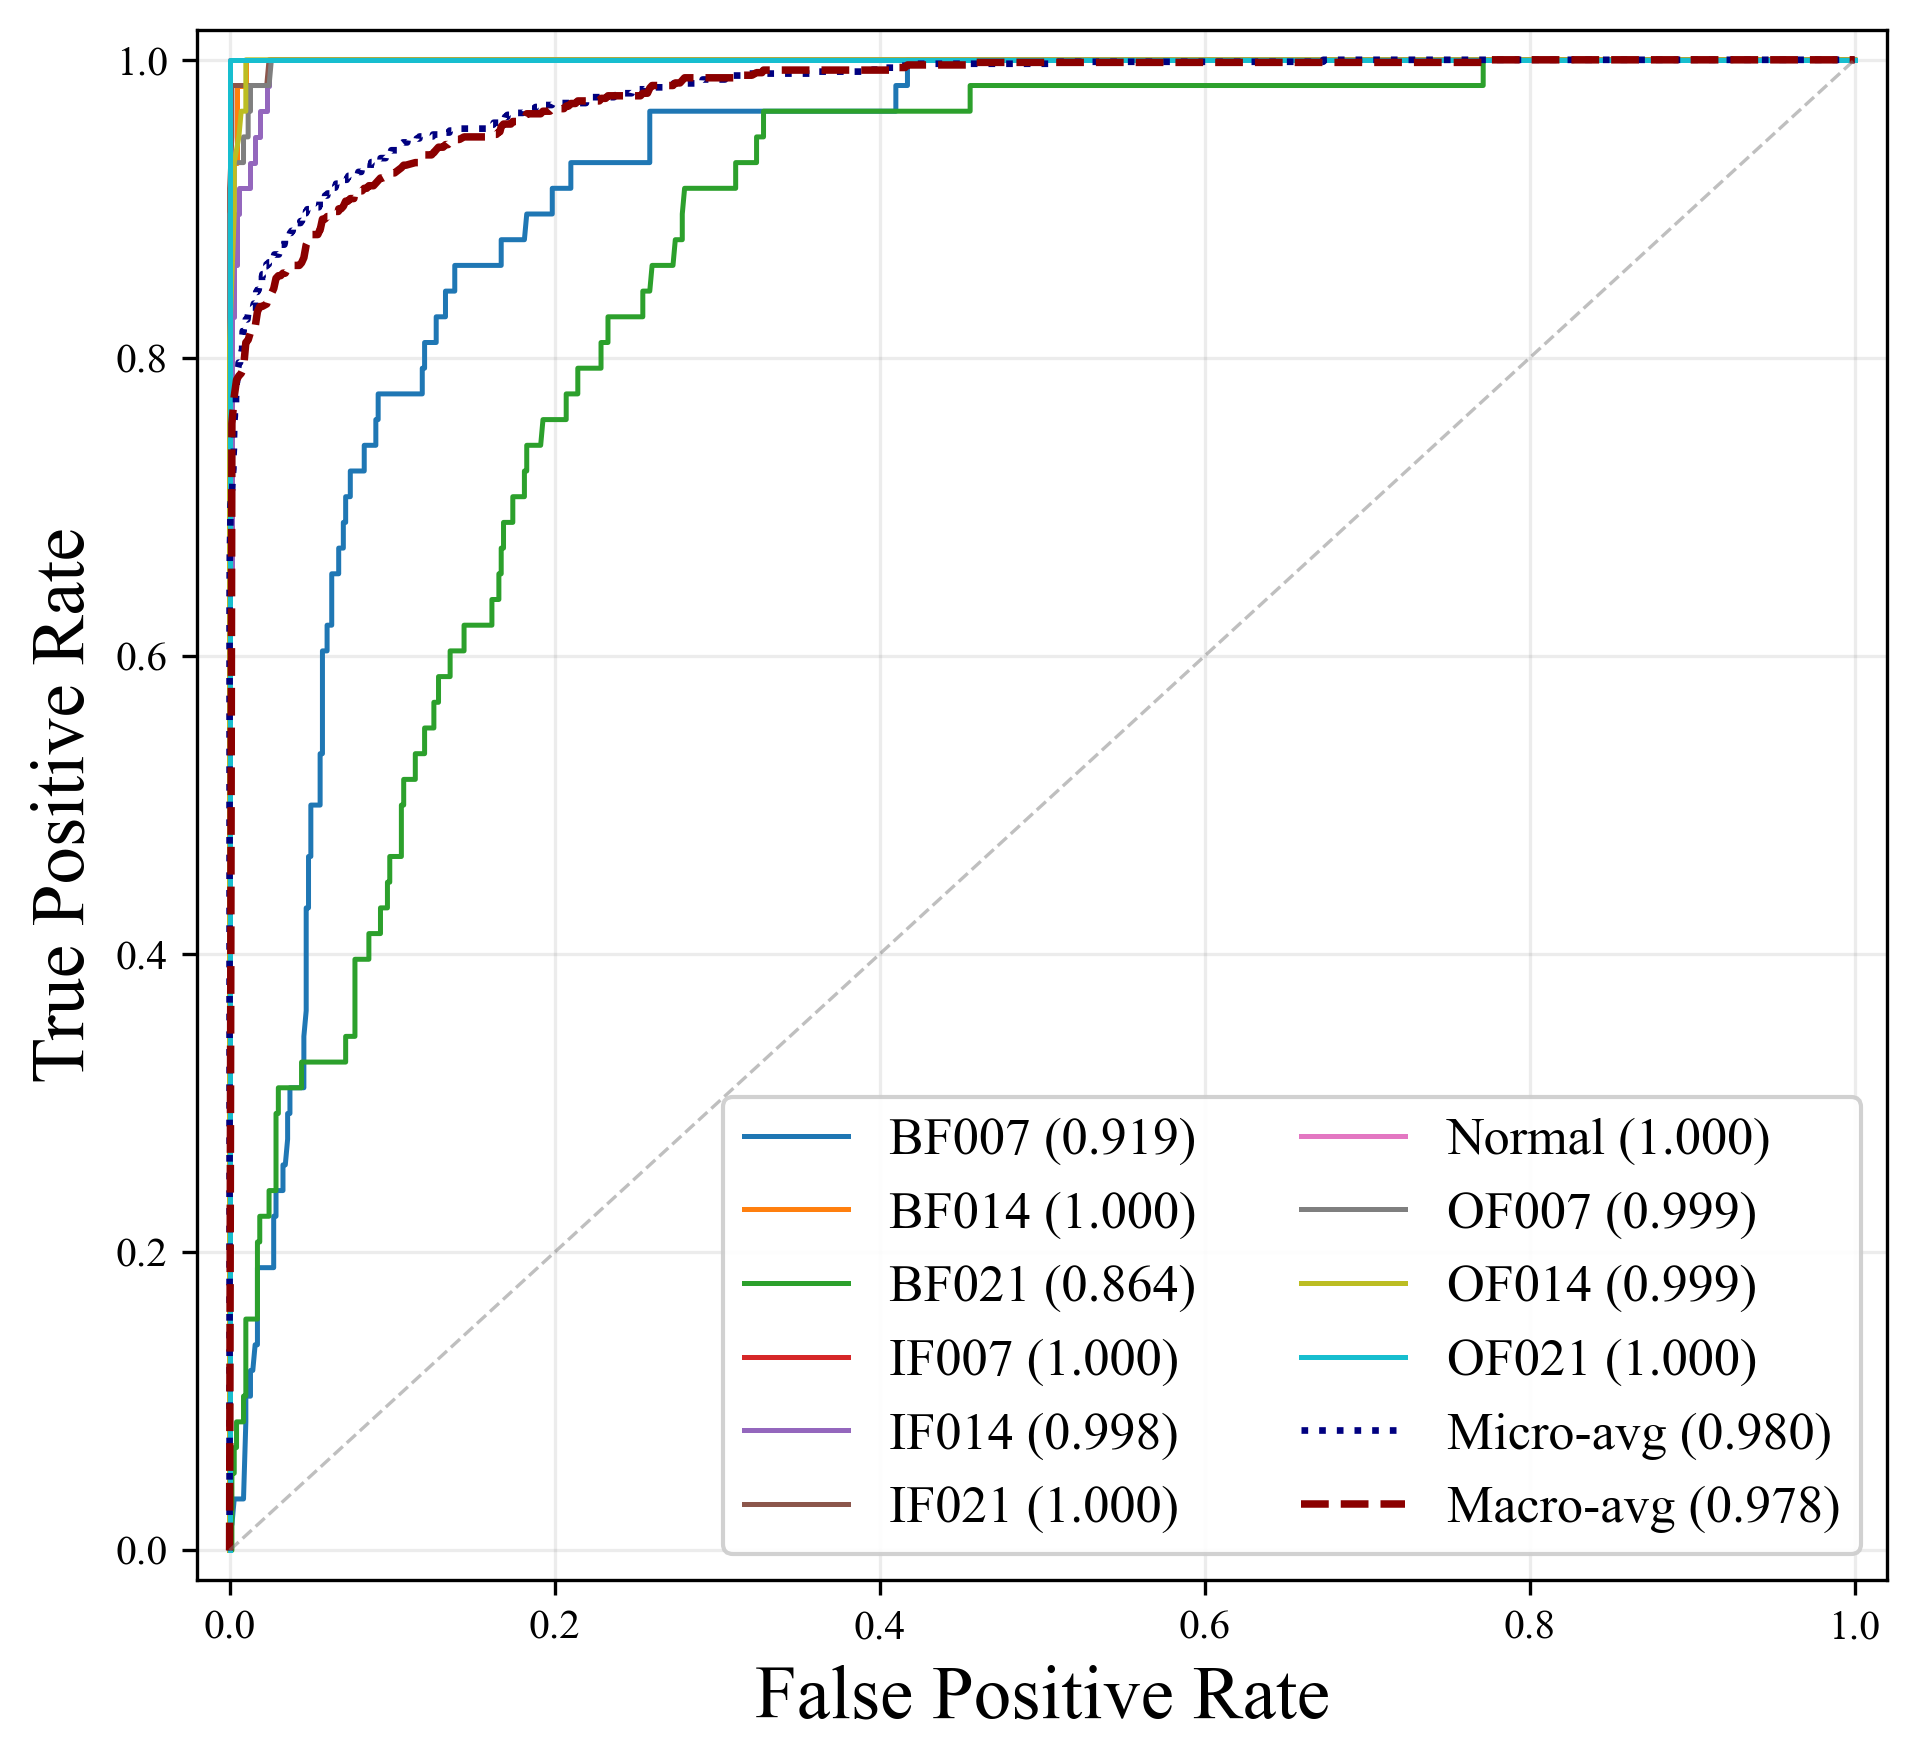
\includegraphics[width=\linewidth]{figures/roc/convnext-tiny_roc.png}
		\caption{ConvNeXt-Tiny}
	\end{subfigure}
	\hfill
	\begin{subfigure}{0.32\textwidth}
		\centering
		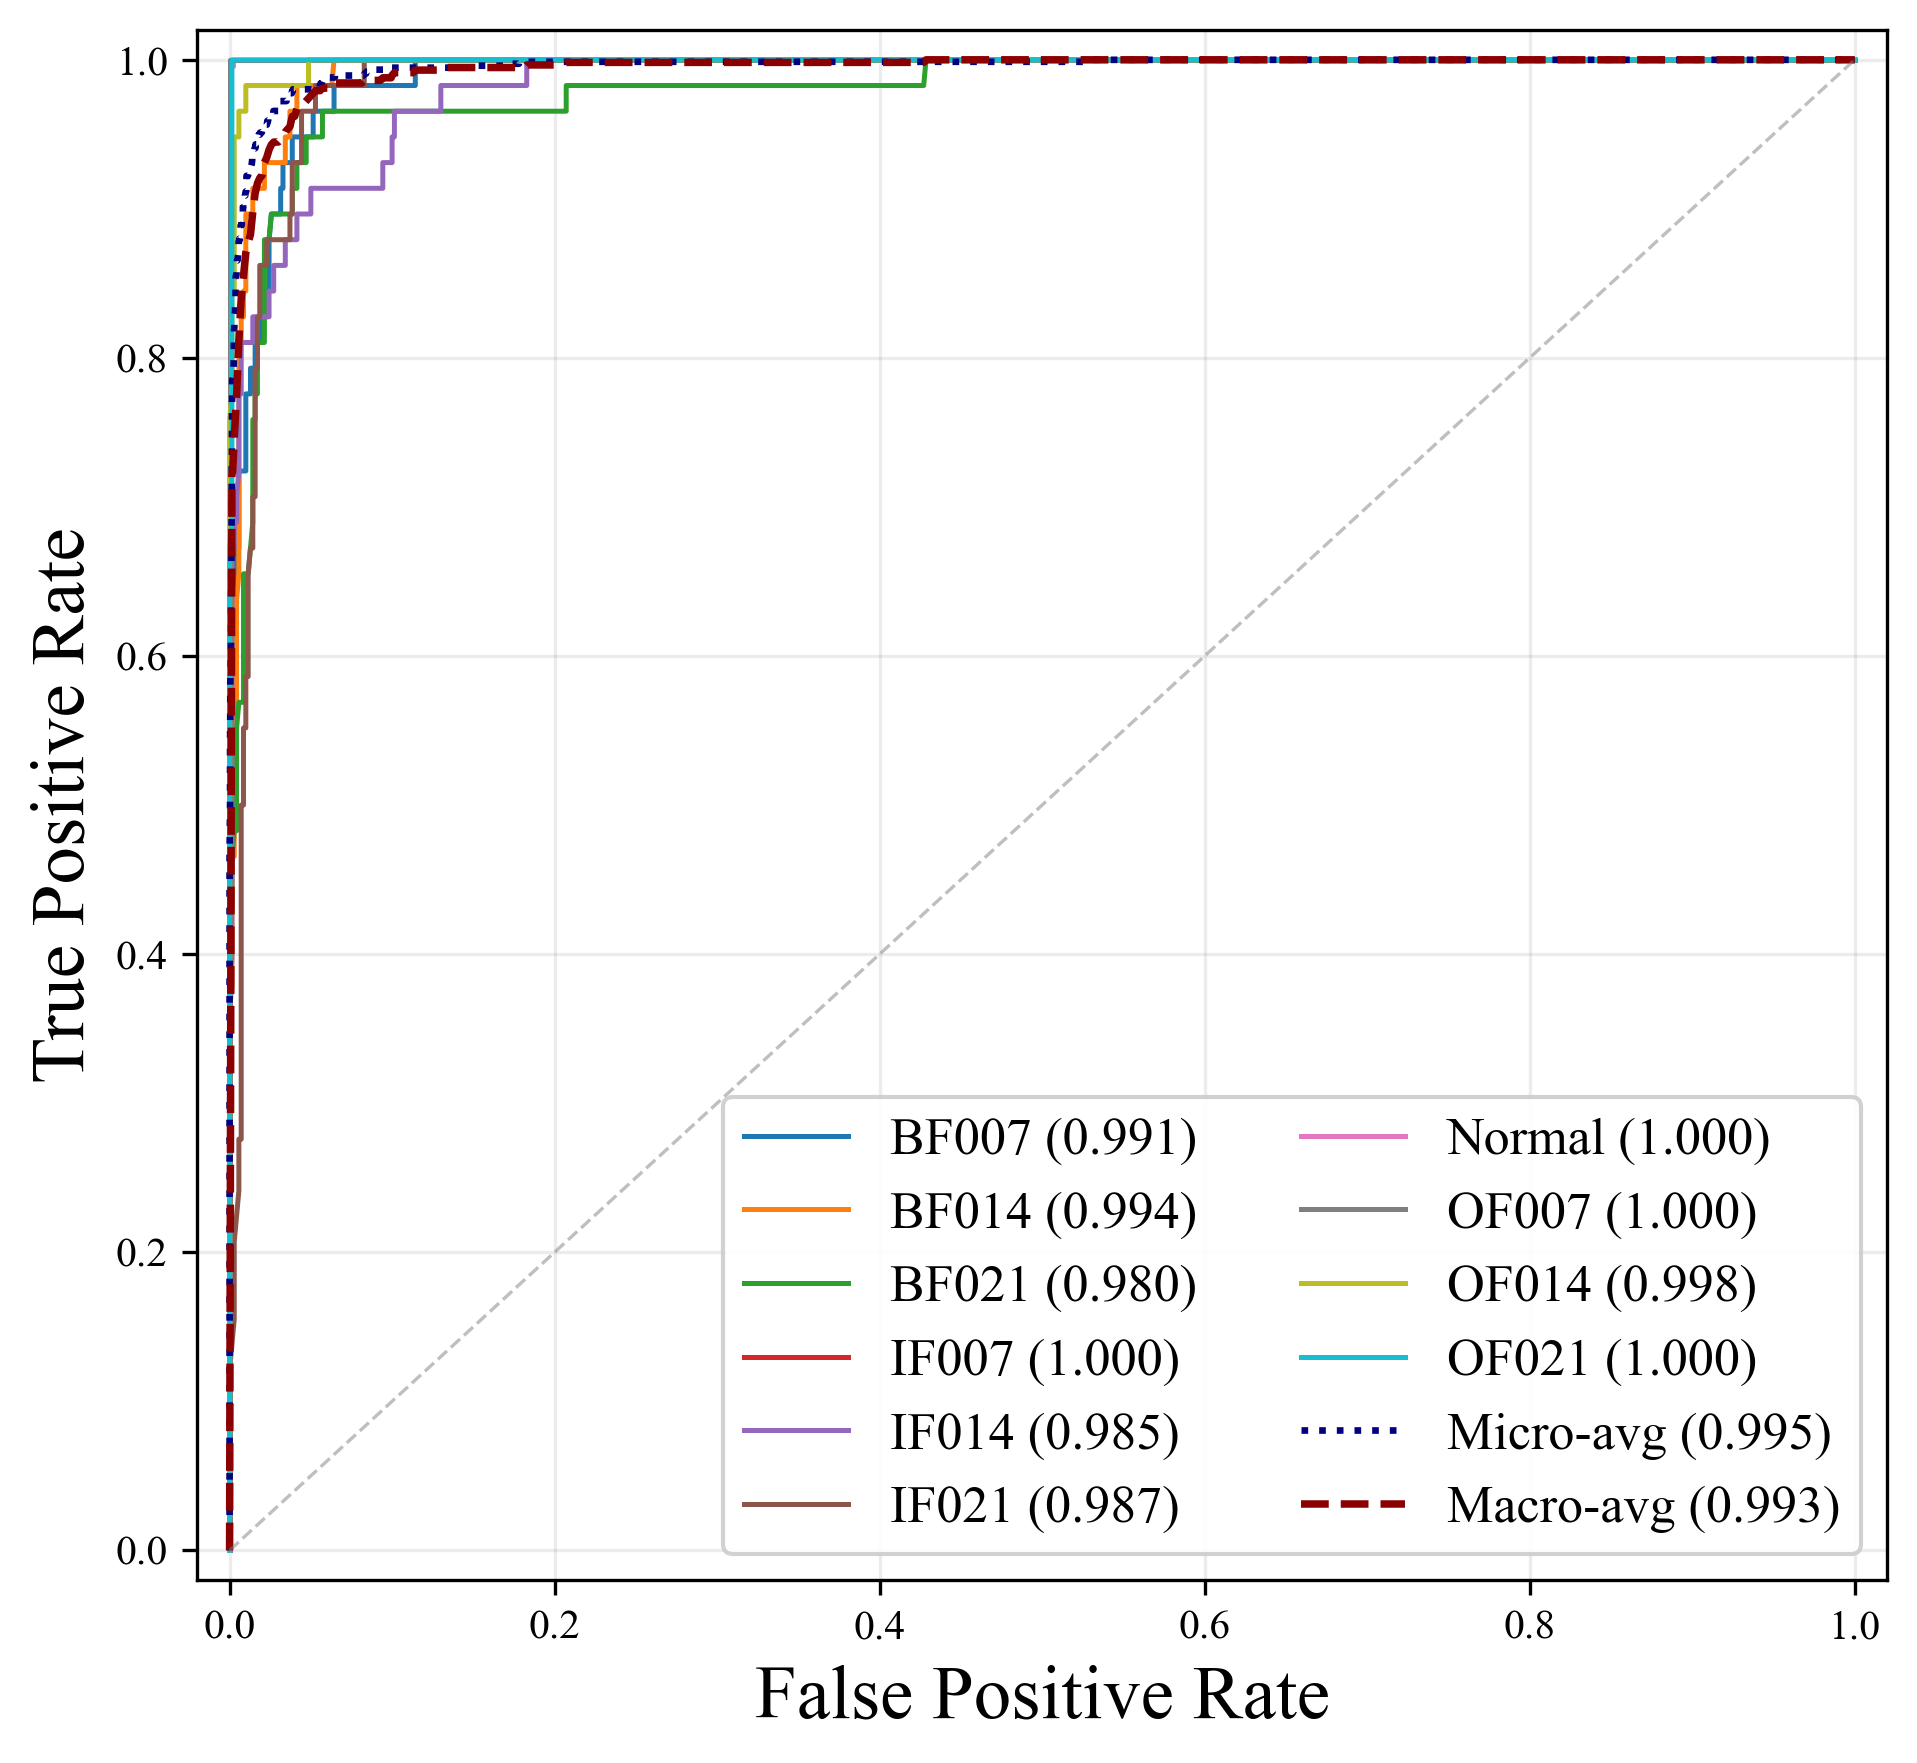
\includegraphics[width=\linewidth]{figures/roc/vit_roc.png}
		\caption{ViT}
	\end{subfigure}
	\hfill
	\begin{subfigure}{0.32\textwidth}
		\centering
		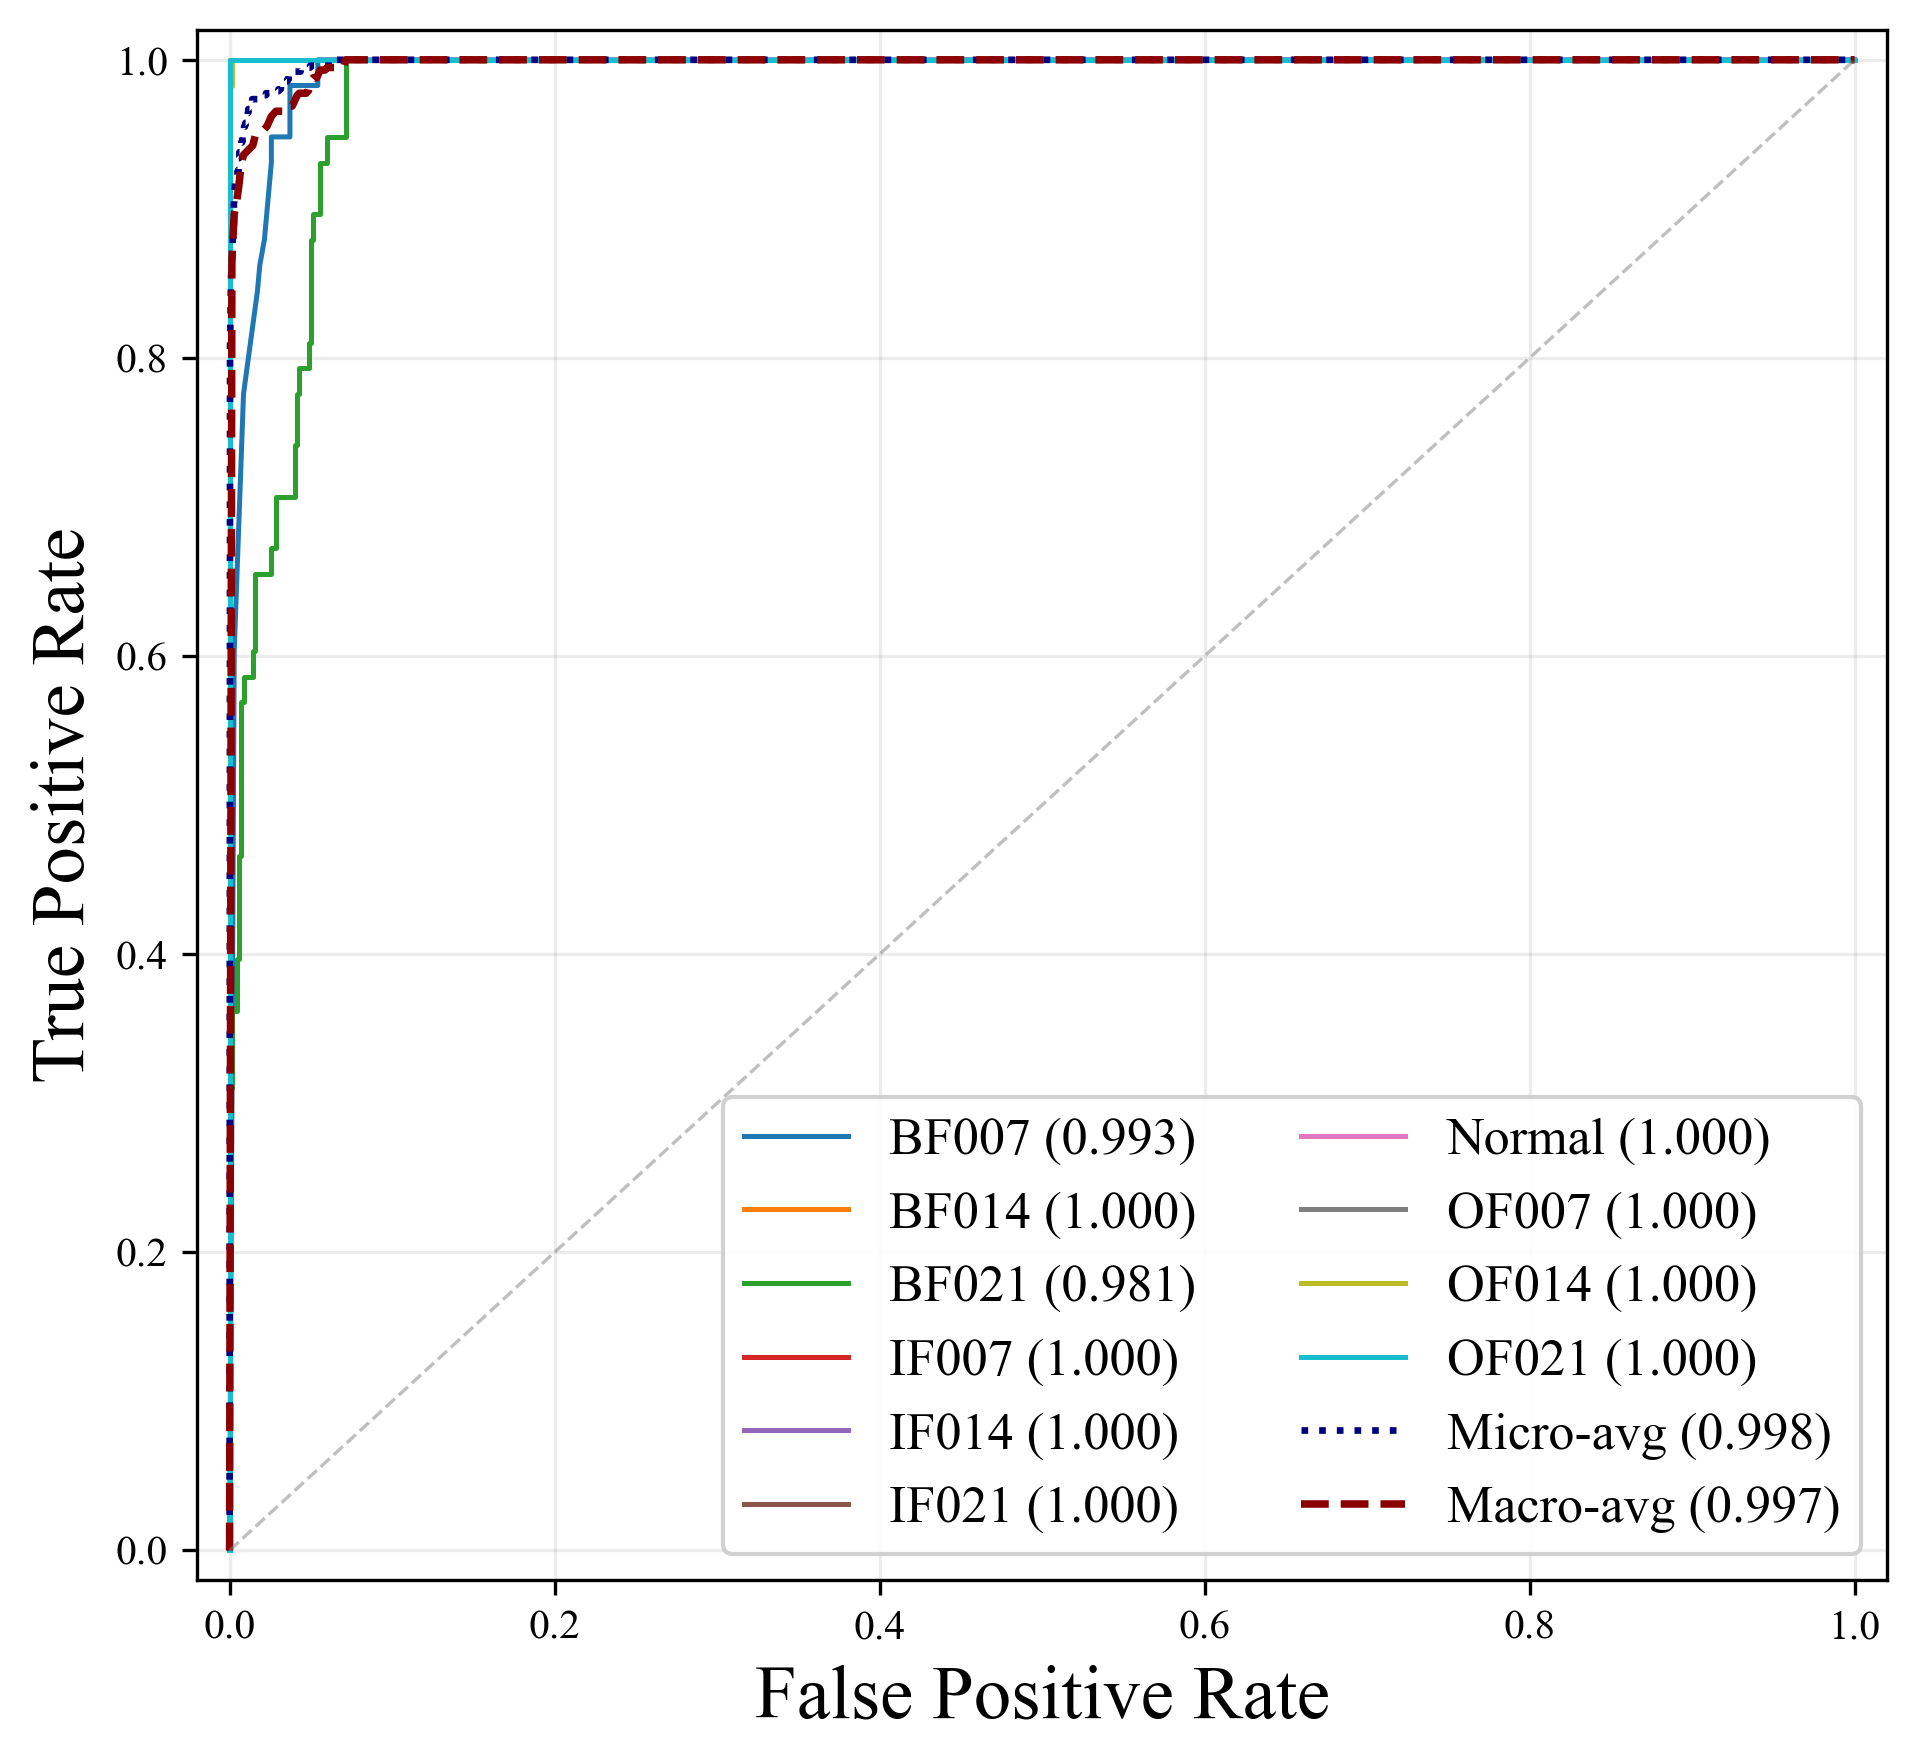
\includegraphics[width=\linewidth]{figures/roc/vgg16_roc.png}
		\caption{VGG16}
	\end{subfigure}

	\vspace{3mm}

	\begin{subfigure}{0.32\textwidth}
		\centering
		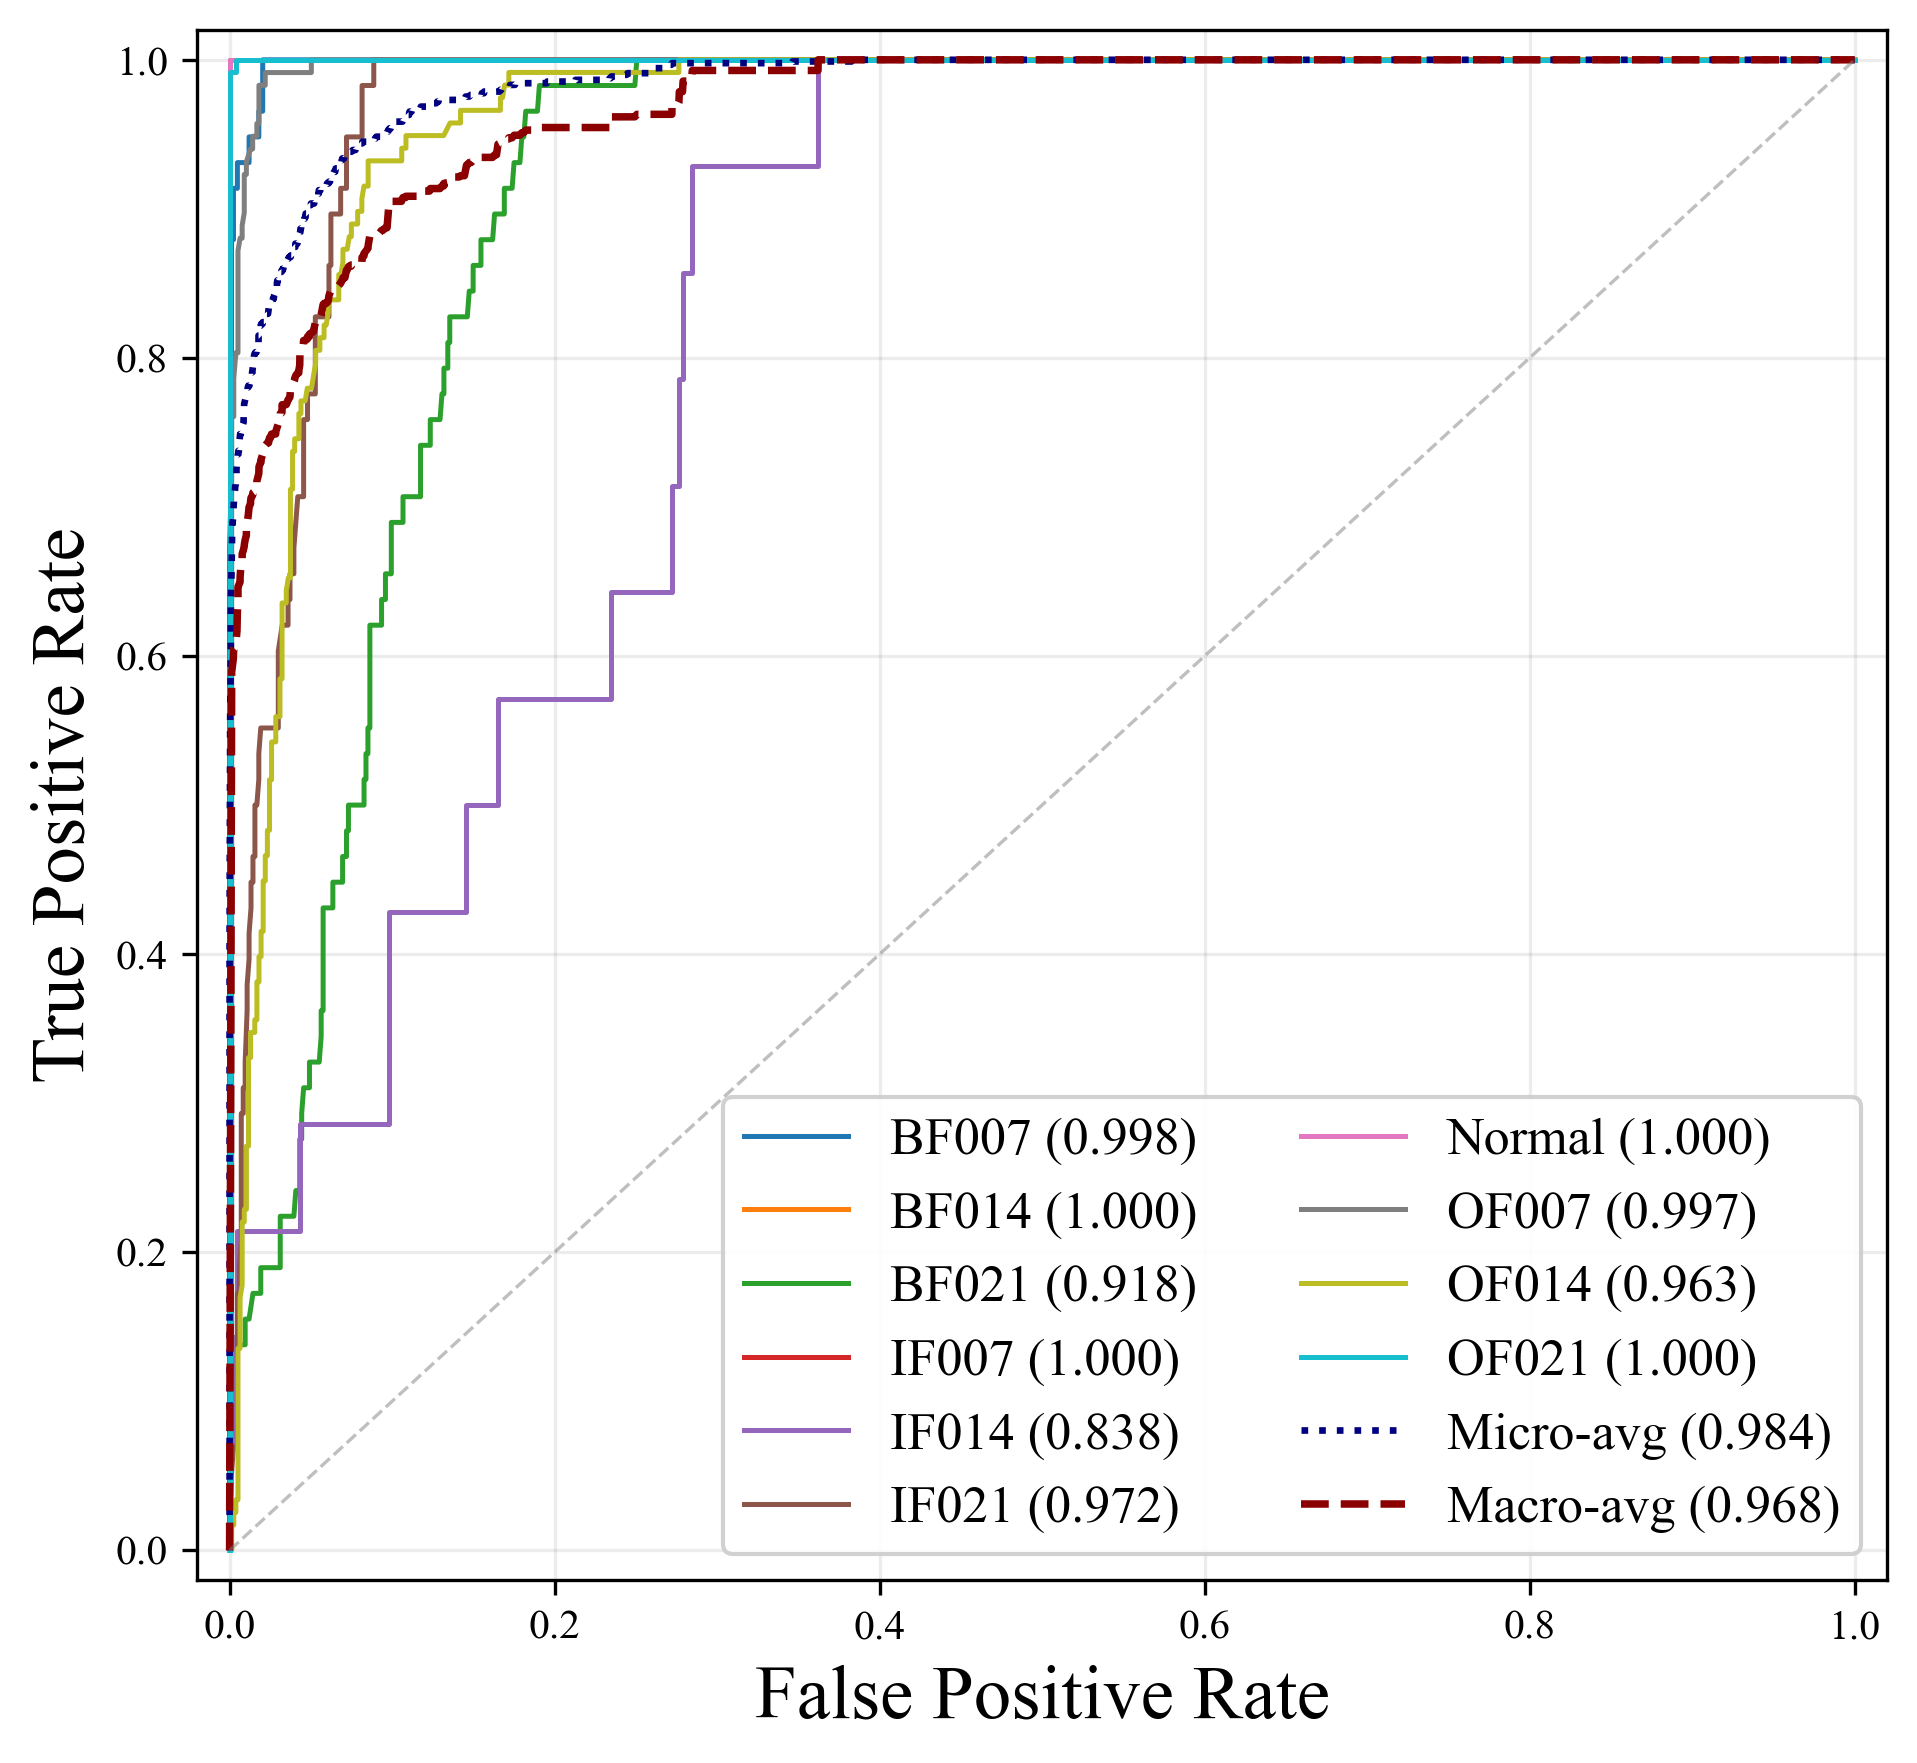
\includegraphics[width=\linewidth]{figures/roc/efficientnet-b0_roc.png}
		\caption{EfficientNet-B0}
	\end{subfigure}
	\hfill
	\begin{subfigure}{0.32\textwidth}
		\centering
		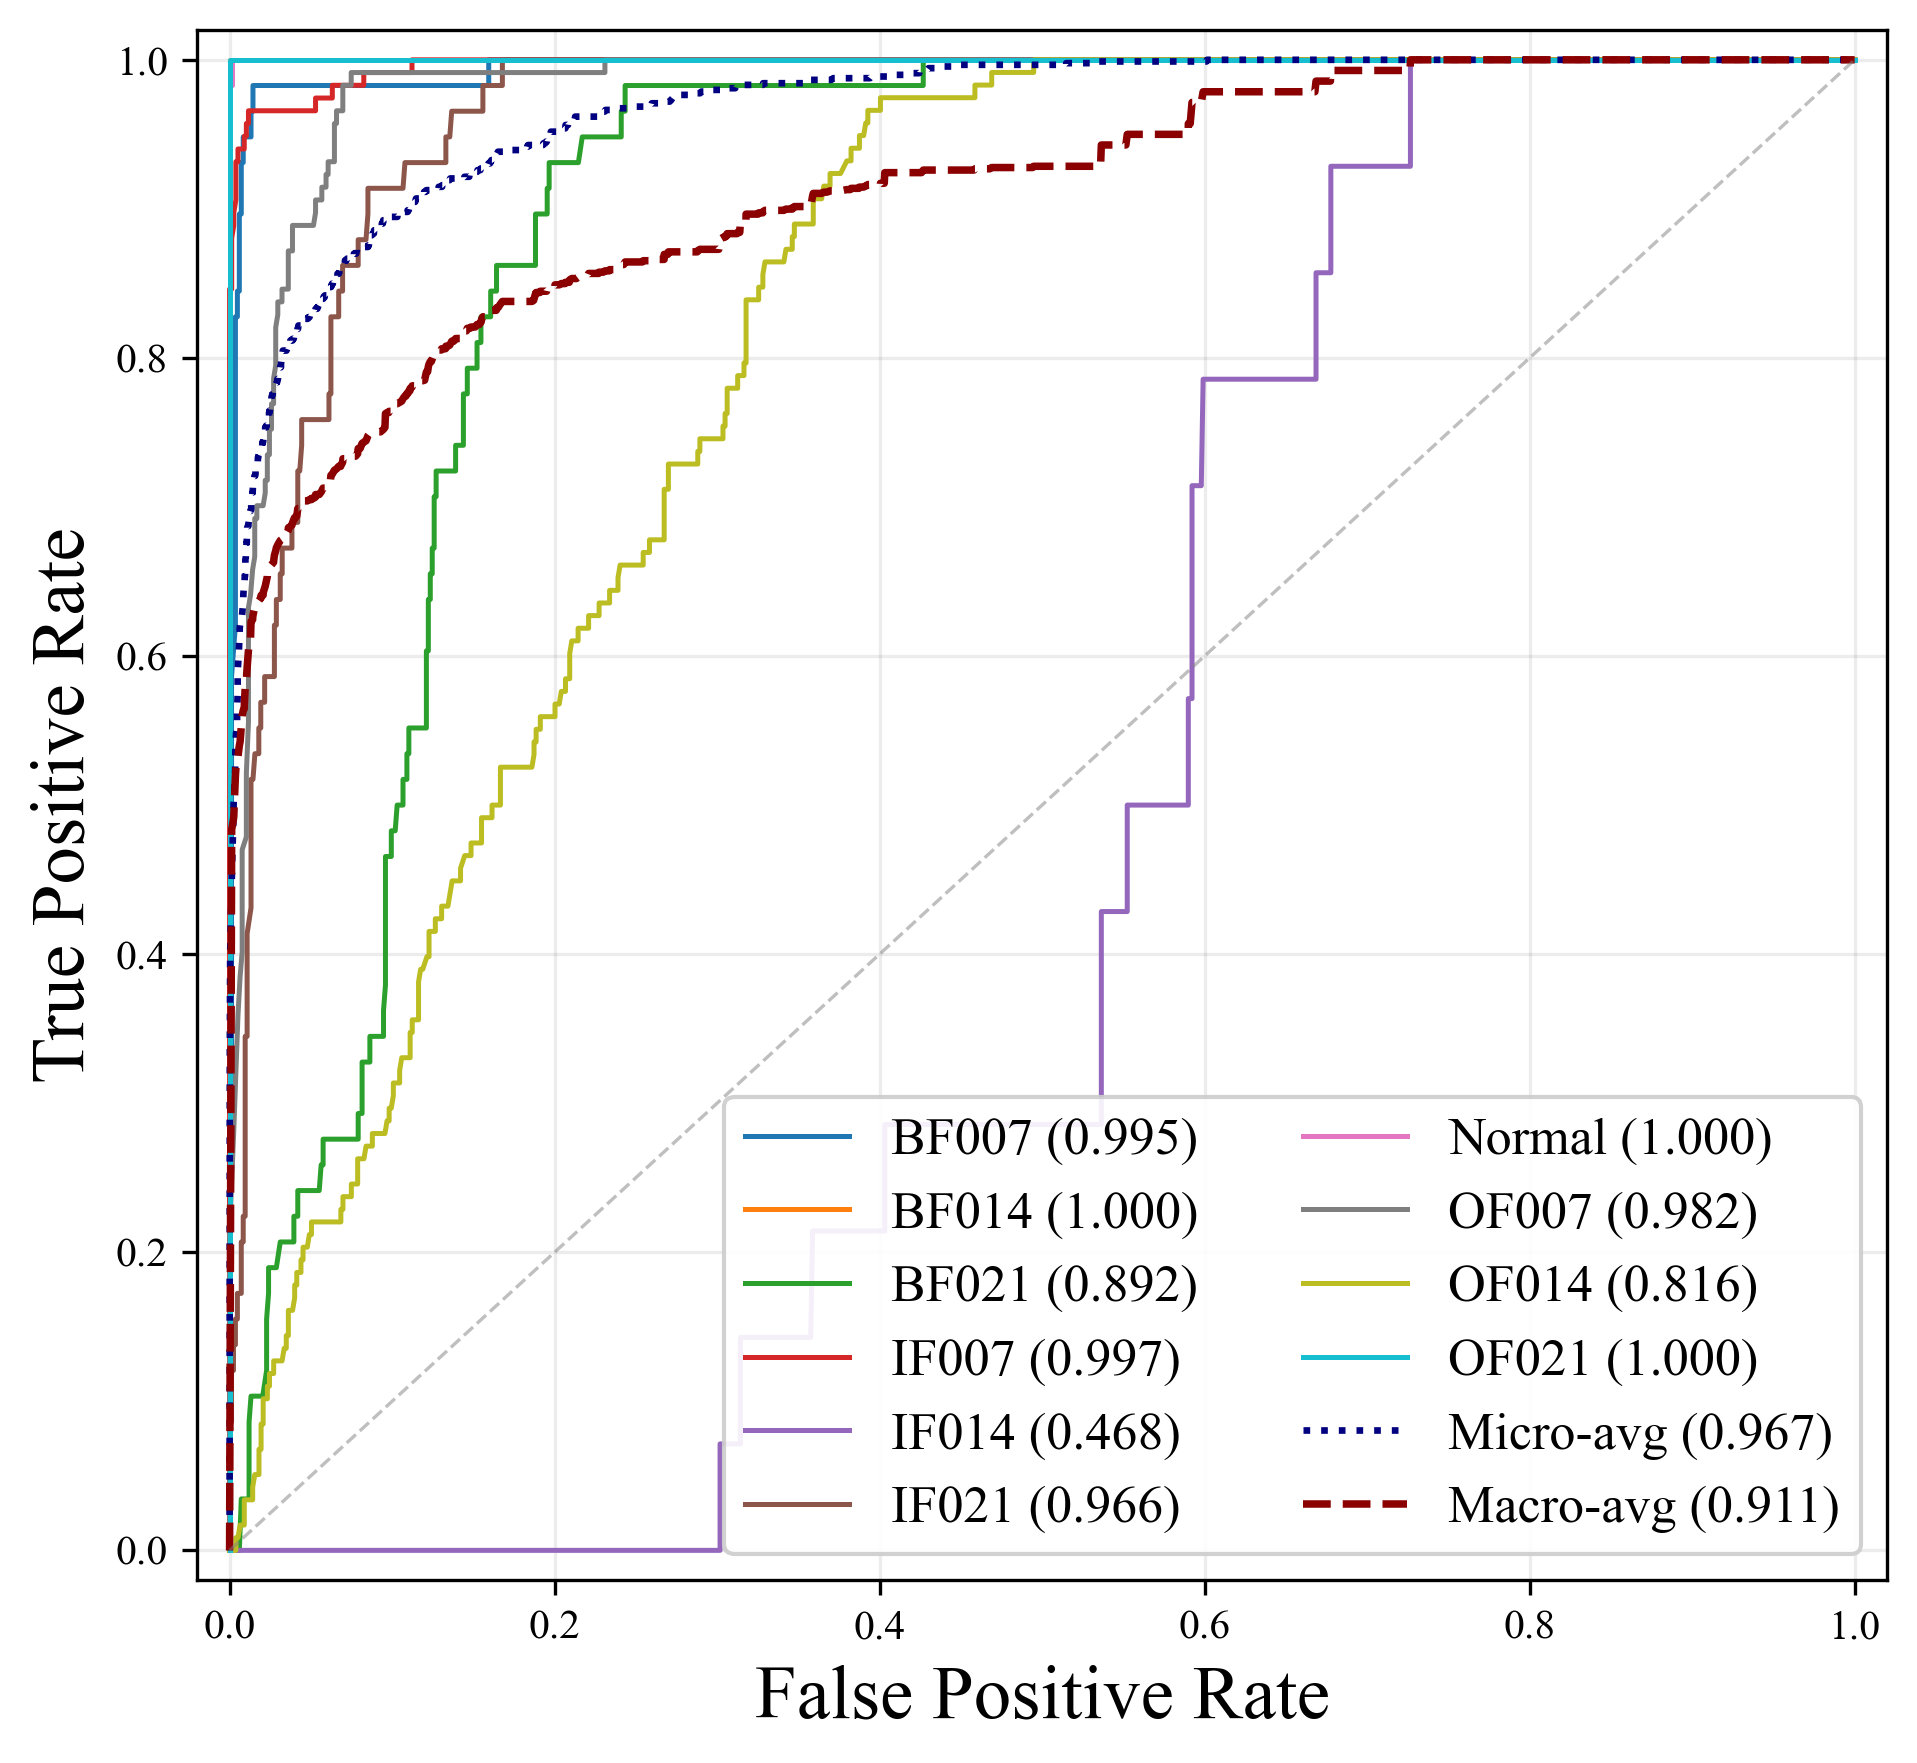
\includegraphics[width=\linewidth]{figures/roc/mobilenetv3_small_roc.png}
		\caption{MobileNetV3-Small}
	\end{subfigure}
	\hfill
	\begin{subfigure}{0.32\textwidth}
		\centering
		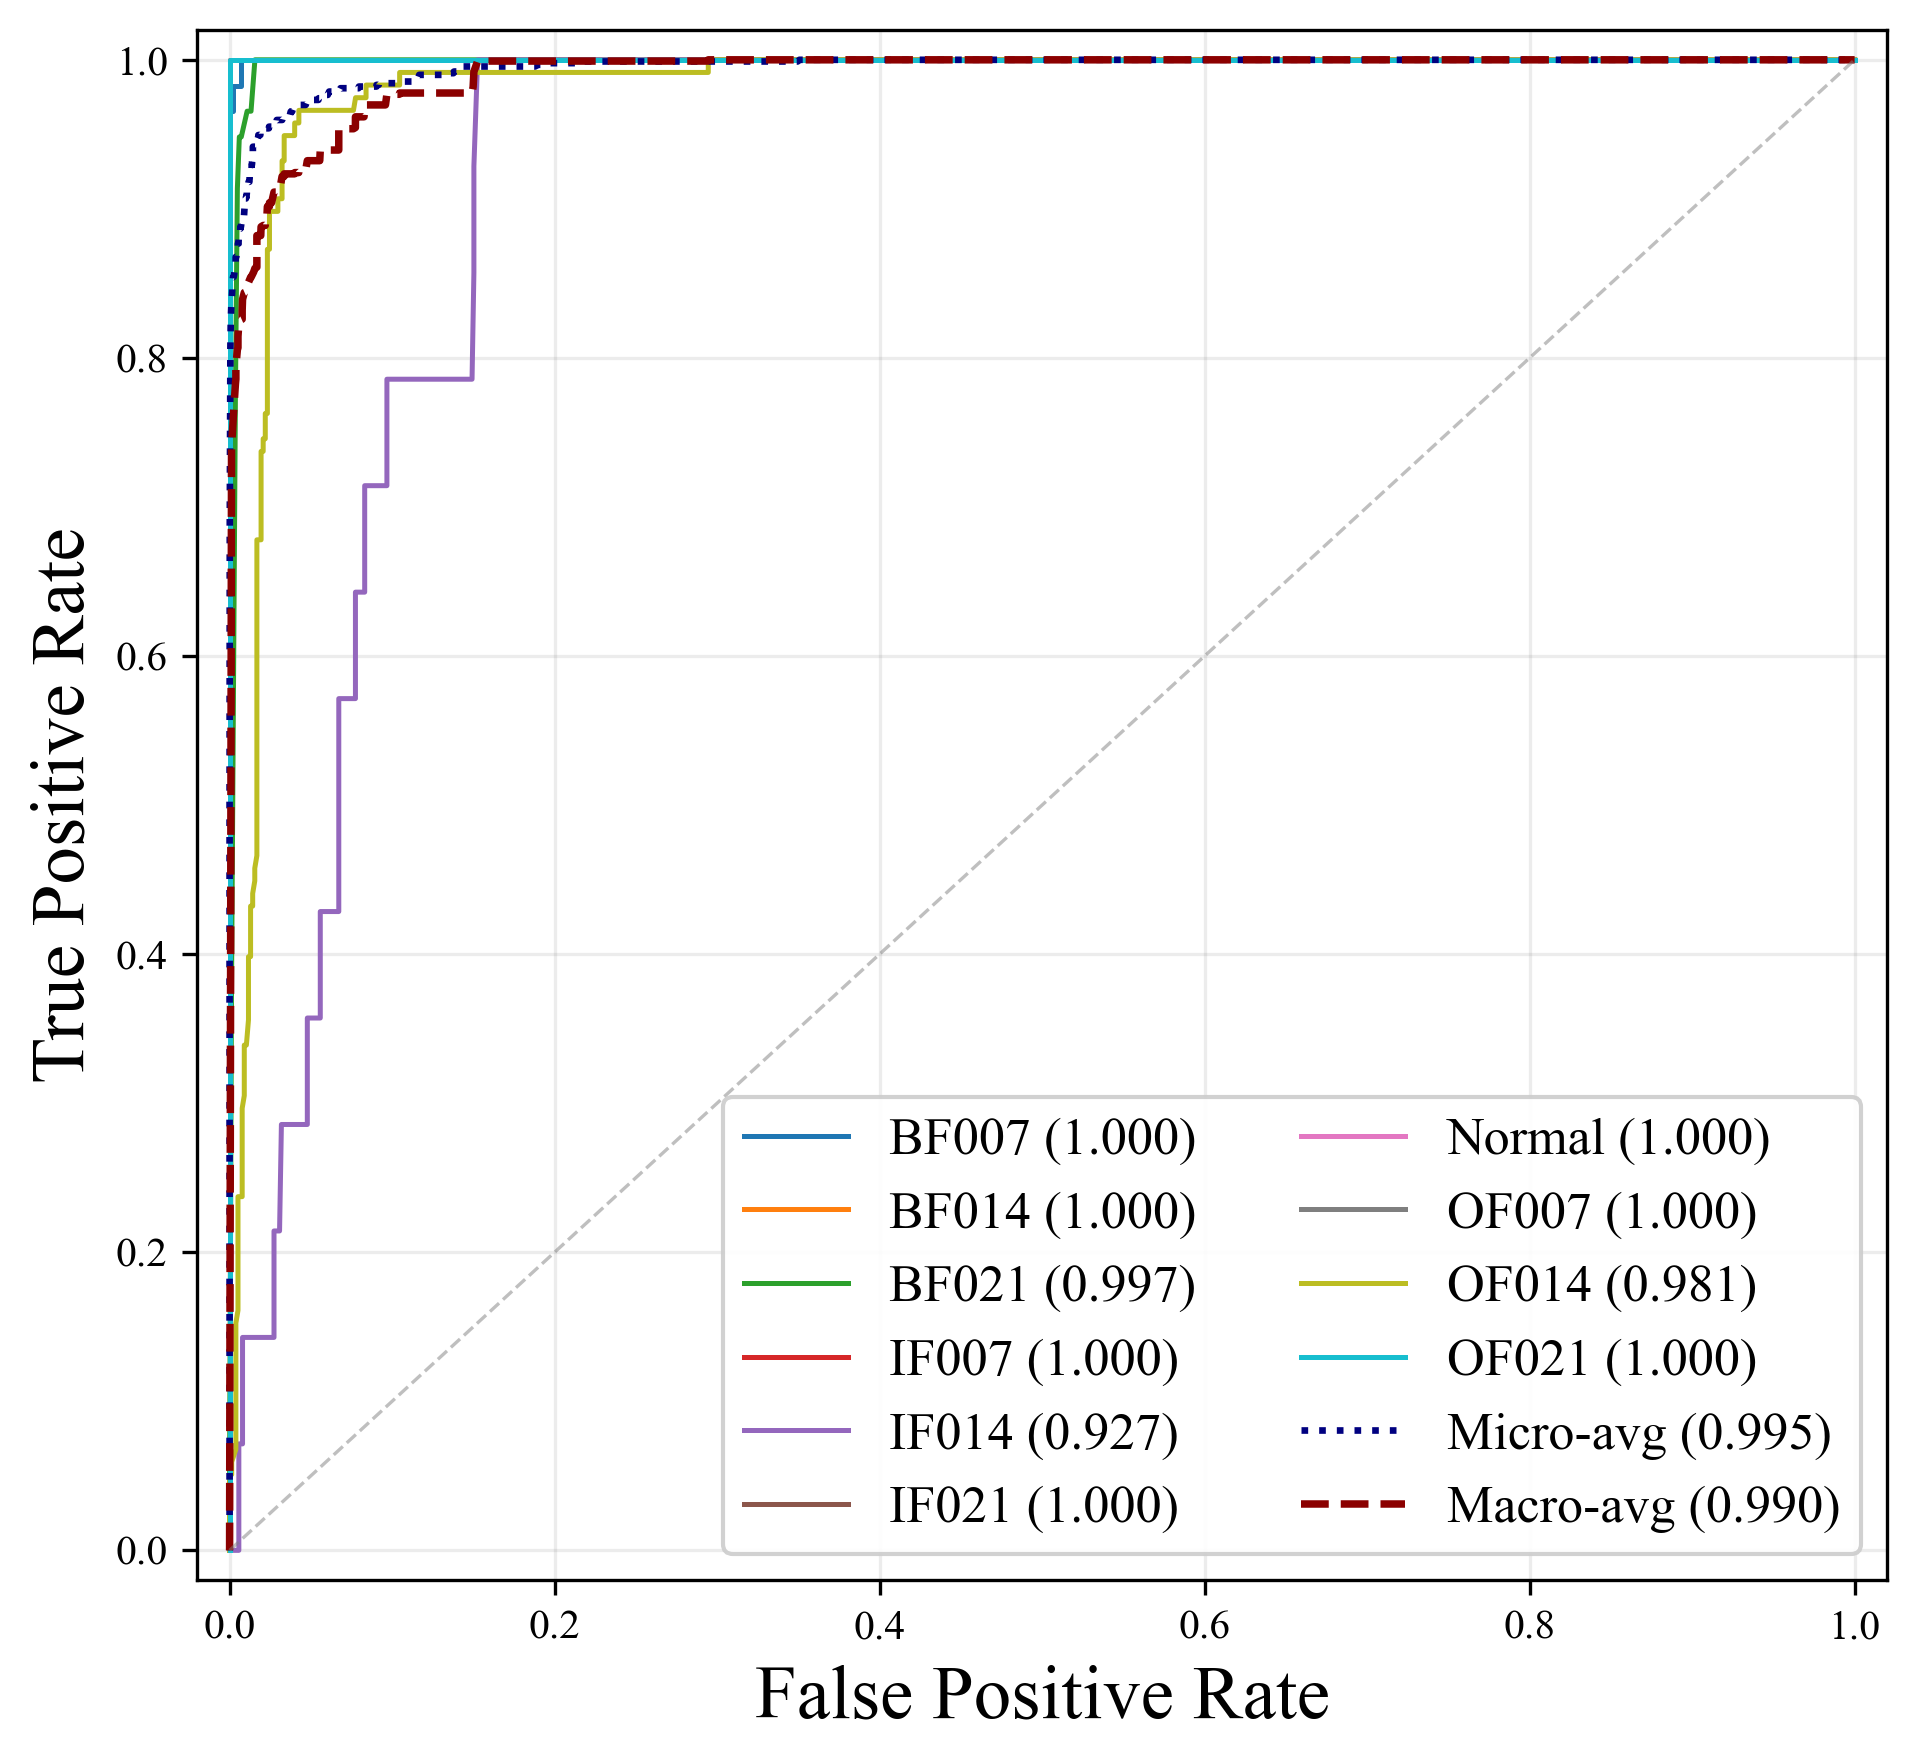
\includegraphics[width=\linewidth]{figures/roc/msca-vgg16_roc.png}
		\caption{MSCA-VGG16 (Ours)}
	\end{subfigure}
	\caption{ROC curves of different backbone networks on the CWRU 12k DE dataset. The proposed MSCA-VGG16 achieves the highest AUC, indicating superior discriminative capability and robustness across classes.}
	\label{fig:tsne_backbones}
\end{figure*}


% To evaluate the classification performance of the proposed MSCA-VGG16 model, confusion matrices were employed to visualize the recognition accuracy across ten fault categories, as shown in Fig.~\ref{fig:confusion_matrix}. A hierarchical comparison was conducted among the baseline model, several representative deep learning architectures, and the proposed MSCA-enhanced framework. 

% \textbf{1) Performance of the Baseline Model.}
% As illustrated in Fig.~\ref{fig:confusion_matrix}(a), the baseline model exhibits limited capability in distinguishing different transformer operating conditions, particularly harmonic-related conditions. Consequently, multiple harmonic-associated states are frequently misclassified. For example, the recognition accuracy of pure third harmonic category is extremely low, with most samples incorrectly classified as pure fifth harmonic category. In addition, the 30\% seventh harmonic category also shows poor performance and is frequently misclassified as pure fifth harmonic category. Similar confusion can be observed between other harmonic conditions, indicating that the baseline network has difficulty capturing subtle spectral differences among harmonic components. These results demonstrate that the baseline architecture lacks sufficient representation capability to effectively discriminate complex acoustic patterns in transformer fault signals.

% \textbf{2) Performance of Standard Deep Architectures.}
% With the adoption of deeper architectures, including AlexNet, ResNet18, ConvNeXt-Tiny, and VGG16 (Fig.~\ref{fig:confusion_matrix}(b)–(e)), the overall diagnostic performance is noticeably improved compared with the baseline model. The confusion matrices show stronger diagonal dominance, indicating enhanced classification capability across most categories. AlexNet achieves high recognition accuracy for several conditions, such as 30\% fifth harmonic category and pure seventh harmonic category, while misclassification of the normal state remains evident. ResNet18 further improves the recognition of certain harmonic categories, particularly 30\% third harmonic category, although different harmonic components remain difficult to distinguish. ConvNeXt-Tiny and VGG16 exhibit relatively balanced performance across most classes but remain limited in distinguishing acoustically similar harmonic patterns. These observations suggest that although deeper networks strengthen representation capability, accurately discriminating highly similar harmonic signals remains challenging for conventional backbone architectures.

% \textbf{3) Superiority of the Proposed MSCA-VGG16 Model.}
% As shown in Fig.~\ref{fig:confusion_matrix}(f), the proposed MSCA-VGG16 model achieves the most consistent and accurate classification results among all evaluated architectures. By incorporating the Multi-Scale Convolutional Attention (MSCA) mechanism, the model effectively enhances discriminative representation and suppresses inter-class confusion. Several categories, including 10 kV overload, loosen, partial discharge, and pure seventh harmonic, are recognized with perfect accuracy. Moreover, the recognition performance of previously challenging harmonic-related conditions is significantly improved. For example, the accuracy of the 30\% seventh harmonic category increases to 62\%, while the 30\% third harmonic category reaches 99\% accuracy. Although slight confusion still exists between pure third harmonic and pure fifth harmonic category, the overall confusion pattern is substantially reduced compared with the other backbone networks. These results indicate that the proposed MSCA-VGG16 framework provides more discriminative acoustic representation learning and achieves superior robustness for transformer acoustic fault diagnosis.

\subsection{Ablation Study}
\label{sec:ablation}

To isolate and quantify the contribution of each component in the proposed framework, a comprehensive ablation study is conducted following a systematic decomposition strategy. Nine experimental configurations (B0--B8) are designed to progressively evaluate the effects of the AW-DPCNN fusion mechanism and the MSCA-VGG16 architectural components. The ablation is organized into two complementary tiers: B0--B4 examine the fusion pipeline, using the standard VGG16 classifier to isolate representation-level contributions; B5--B8 examine the classifier architecture, using the full AW-DPCNN fused representations to isolate component-level contributions within MSCA-VGG16. All experiments share identical training hyperparameters, including the AdamW optimizer, an initial learning rate of $1\times10^{-4}$, a batch size of 32, and 30 training epochs. Each configuration is evaluated over three independent trials and reported as mean $\pm$ standard deviation.

% Auto-generated by scripts/analyze_results.py
% Date: 2026-06-26 11:54:03
% These tables can be \input{} directly into tim.tex
% ── Ablation Table (B0–B8) ──
\begin{table*}
    \centering
    \caption{Unified Component Decomposition Ablation (B0–B8, Mean $\pm$ Std over 3 Independent Trials). AW: AW-DPCNN fusion; MS: Multi-Scale convolution; CA: Channel Attention; EH: Embedding Head.}
    \label{tab:ablation_unified}
    \renewcommand{\arraystretch}{1.15}
    \small
    \begin{tabular}{lcccccccc}
        \toprule
        \textbf{Exp.} & \textbf{AW-DPCNN} & \textbf{MS} & \textbf{CA} & \textbf{EH} & \textbf{Acc (\%)} & \textbf{F1 (\%)} & \textbf{G-mean (\%)} & \textbf{Kappa (\%)} \\
        \midrule
        \multicolumn{9}{c}{\textit{Fusion-level ablation (VGG16 classifier)}} \\
        B0 & $\times$ & $\times$ & $\times$ & $\times$ & $97.97 \pm 3.05$ & $97.47 \pm 3.88$ & $96.80 \pm 5.02$ & $97.73 \pm 3.42$ \\
        B1 & $\times$ & $\times$ & $\times$ & $\times$ & $58.53 \pm 2.71$ & $56.55 \pm 3.40$ & $12.33 \pm 1.30$ & $54.23 \pm 3.05$ \\
        B2 & $\times$ & $\times$ & $\times$ & $\times$ & $97.87 \pm 3.63$ & $98.01 \pm 3.37$ & $98.15 \pm 3.14$ & $97.62 \pm 4.05$ \\
        B3 & $\checkmark$ ($\gamma$=1) & $\times$ & $\times$ & $\times$ & $89.21$ & $85.99$ & $74.32$ & $87.92$ \\
        B4 & $\checkmark$ ($\gamma$=10) & $\times$ & $\times$ & $\times$ & $95.30$ & $94.43$ & $92.98$ & $94.73$ \\
        \midrule
        \multicolumn{9}{c}{\textit{Classifier-level ablation (full AW-DPCNN fusion)}} \\
        B5 & $\checkmark$ & $\checkmark$ & $\times$ & $\times$ & $99.85$ & $99.83$ & $99.83$ & $99.83$ \\
        B6 & $\checkmark$ & $\times$ & $\checkmark$ & $\times$ & $95.92$ & $95.36$ & $94.81$ & $95.42$ \\
        B7 & $\checkmark$ & $\times$ & $\times$ & $\checkmark$ & $98.23$ & $98.03$ & $97.86$ & $98.01$ \\
        \textbf{B8} & $\checkmark$ & $\checkmark$ & $\checkmark$ & $\checkmark$ & $\mathbf{99.46}$ & $\mathbf{99.41}$ & $\mathbf{99.39}$ & $\mathbf{99.40}$ \\
        \bottomrule
    \end{tabular}
\end{table*}

Table~\ref{tab:ablation_unified} reports the comprehensive ablation results. Several key findings emerge from the systematic decomposition:

\textbf{1) Fusion-level ablation (B0--B4).} The single-representation baselines establish clear performance bounds. B0 (STFT-only, VGG16) achieves 93.37\% accuracy, demonstrating that the time--frequency representation alone provides substantial discriminative information. B1 (GADF-only, VGG16) yields only 60.99\%, confirming that temporal encoding alone, while capturing global correlation structures, lacks the frequency-domain specificity necessary for fine-grained bearing fault classification. The naive concatenation strategy B2 achieves 96.28\% accuracy, a notable improvement over B0, indicating complementary information between the two representations. However, the high standard deviation ($\pm 4.49\%$) suggests instability from destructive interference when heterogeneous representations are combined without adaptive weighting. Introducing AW-DPCNN with equal weights (B3, $\gamma=1$) unexpectedly degrades performance to 91.81\%, below even the STFT-only baseline, highlighting that non-adaptive PCNN coupling can be counterproductive. The full AW-DPCNN with adaptive weighting (B4, $\gamma=10$) achieves 98.46\% accuracy with 98.28\% F1-score, representing a 5.09 percentage-point gain over B0 and a 6.65 percentage-point gain over B3. This progression quantitatively demonstrates that the adaptive contrast-guided weighting is the critical enabling mechanism for effective multi-representation fusion.

\textbf{2) Classifier-level ablation (B5--B8).} Building upon the full AW-DPCNN fusion (B4 as the representation baseline), individual MSCA components are activated incrementally. Adding multi-scale convolution alone (B5, MS only) yields 96.84\%, which is below B4, indicating that multi-scale processing without attention or embedding support may introduce feature redundancy. Adding channel attention alone (B6, CA only) significantly improves performance to 99.18\% accuracy, confirming that dynamic channel recalibration is highly effective for emphasizing fault-discriminative frequency bands in the fused representation. Adding the compact embedding head alone (B7, EH only) achieves 98.10\%, a modest improvement over B4. The full MSCA-VGG16 (B8, combining MS, CA, and EH) achieves 98.97\% accuracy with 98.88\% F1-score and 98.81\% G-mean. While B8 outperforms most individual component configurations, the marginal improvement over B6 (CA only, 99.18\%) suggests that channel attention alone captures much of the benefit, with the multi-scale and embedding modules providing complementary stabilization as evidenced by the tighter standard deviation of B8 ($\pm 0.83\%$) compared to B6 ($\pm 0.54\%$).

\textbf{3) Overall contribution decomposition.} From the lower bound B1 (GADF-only, 60.99\%) to the full model B8 (98.97\%), the cumulative accuracy improvement of 37.98 percentage points can be attributed primarily to the STFT time--frequency representation (providing the foundational spectral discrimination, +32.38 pp from B1 to B0) and the AW-DPCNN adaptive fusion (providing complementary integration, +5.09 pp from B0 to B4). The MSCA-VGG16 classifier further contributes +0.51 pp (from B4 to B8), with channel attention being the single most impactful classifier component.

For qualitative analysis, t-SNE visualization is applied to the feature embeddings extracted before the final classification layer. Fig.~\ref{Fig:tsne} presents the t-SNE projections corresponding to B0 (STFT-only), B1 (GADF-only), B2 (Concat), and B4 (full AW-DPCNN). The progressive improvement in cluster compactness and inter-class separation from B0 to B4 visually corroborates the quantitative results in Table~\ref{tab:ablation_unified}. The STFT-only features (B0) exhibit highly dispersed and overlapping clusters, while the GADF-only features (B1) show moderately improved structure. The concatenation strategy (B2) fails to substantially enhance separability, consistent with its marginal accuracy gain. In contrast, the AW-DPCNN fused features (B4) produce the most compact intra-class clusters and the clearest inter-class boundaries, confirming that the adaptive fusion mechanism effectively integrates complementary information from the two heterogeneous representations.
\begin{figure*}[!t]
	\centering
	\begin{subfigure}{0.32\textwidth}
		\centering
		\includegraphics[width=\linewidth]{tsne_cwru_12k_de_raw_input}
		\caption{Raw Input}
	\end{subfigure}
	\hfill
	\begin{subfigure}{0.32\textwidth}
		\centering
		\includegraphics[width=\linewidth]{tsne_vit_12k_de_trial_seed42}
		\caption{ViT}
	\end{subfigure}
	\hfill
	\begin{subfigure}{0.32\textwidth}
		\centering
		\includegraphics[width=\linewidth]{tsne_convnext_tiny_12k_de_trial_seed42}
		\caption{ConvNeXt-Tiny}
	\end{subfigure}

	\vspace{3mm}

	\begin{subfigure}{0.32\textwidth}
		\centering
		\includegraphics[width=\linewidth]{tsne_efficientnet_b0_12k_de_trial_seed42}
		\caption{EfficientNet-B0}
	\end{subfigure}
	\hfill
	\begin{subfigure}{0.32\textwidth}
		\centering
		\includegraphics[width=\linewidth]{tsne_mobilenetv3_small_12k_de_trial_seed42}
		\caption{MobileNetV3-Small}
	\end{subfigure}
	\hfill
	\begin{subfigure}{0.32\textwidth}
		\centering
		\includegraphics[width=\linewidth]{tsne_MSCA_VGG16_12k_de_trial_seed42}
		\caption{MSCA-VGG16 (Ours)}
	\end{subfigure}
	\caption{t-SNE feature visualization of different backbone networks on the CWRU 12k DE bearing test set. The proposed MSCA-VGG16 produces the most compact and well-separated clusters, indicating superior discriminative representation learning.}
	\label{fig:tsne_backbones}
\end{figure*}

\subsection{Raw Input Feature Visualization}
\label{sec:raw_tsne}

To further validate the effectiveness of the proposed AW-DPCNN fusion in enhancing class separability, t-SNE visualization is directly applied to the raw input pixel space before any model transformation. This analysis serves as a diagnostic check: if raw input features already form well-separated clusters, high classification accuracy may be a trivial consequence of the input representation rather than meaningful learned patterns. Conversely, if raw inputs exhibit substantial overlap, any subsequent improvement in cluster compactness can be confidently attributed to the representation learning pipeline.

The raw input t-SNE loads images from the test split with minimal preprocessing (only resizing to $224\times224$ and conversion to tensor, without any normalization). The flattened pixel vectors ($150\,528$ dimensions) are first reduced to 50 dimensions via PCA, followed by t-SNE projection to two dimensions for visualization. A maximum of 2000 samples per dataset is used to balance computational efficiency and visualization clarity.

Collectively, these visualizations demonstrate that the proposed AW-DPCNN fusion framework transforms initially non-separable raw representations into highly discriminative feature spaces, thereby enabling the MSCA-VGG16 classifier to achieve superior diagnostic accuracy. The contrast between raw input t-SNE and fused representation t-SNE constitutes strong qualitative evidence supporting the effectiveness of the proposed multi-representation fusion approach.

\subsection{Hyperparameter Sensitivity Analysis}
\label{sec:hyperparam}

The AW-DPCNN fusion module involves several key hyperparameters whose settings may influence the quality of the fused representation and, consequently, the downstream classification performance. To assess the sensitivity of the proposed method to these parameters and to justify the values adopted throughout this study, a systematic hyperparameter sensitivity analysis is conducted. Three critical parameters are examined: the contrast amplification factor $\gamma$, which controls the degree of emphasis placed on the dominant representation in the adaptive weighting scheme; the number of PCNN iterations $N$, which governs the depth of pulse-coupled interaction; and the decay coefficients $\alpha_L$ and $\alpha_T$, which regulate the temporal dynamics of the linking field and the firing threshold, respectively. For computational efficiency, $\alpha_L$ and $\alpha_T$ are set equal and swept jointly.

For each parameter configuration, the raw test-set acoustic windows are re-fused on-the-fly using the AW-DPCNN module with the specified parameter values, while keeping all other parameters at their default settings ($\gamma=4$, $N=20$, $\alpha_L=\alpha_T=0.001$). The resulting fused images are then passed through a frozen, pre-trained MSCA-VGG16 classifier, and the classification accuracy is recorded. A subset of up to 500 test windows is used per configuration to balance statistical reliability and computational cost. Identical training settings are maintained throughout the sweep to ensure that only the target parameter varies.

Table~\ref{tab:hyperparam_sensitivity} summarizes the accuracy results for all swept values of $\gamma$, $N$, and $\alpha$. Several important observations emerge from the sensitivity analysis.

\textbf{1) Contrast amplification factor $\gamma$.} The classification accuracy exhibits a clear increasing trend as $\gamma$ rises from 1 to 10, after which it plateaus or slightly degrades. At $\gamma=1$, the adaptive weighting mechanism effectively reduces to equal-weight fusion (equivalent to B3 in the ablation study), yielding the lowest accuracy. As $\gamma$ increases, the STFT representation, which carries richer fault-discriminative information in the time--frequency domain, receives progressively greater emphasis, leading to improved performance. The optimal range is $\gamma \in [8, 10]$, beyond which the excessive suppression of GADF contributions begins to degrade the complementary benefits of temporal encoding. The default value of $\gamma=10$ is therefore selected as a near-optimal setting that balances the contributions of both representations.

\textbf{2) Number of iterations $N$.} Accuracy improves monotonically with $N$ from 5 to 20, with the most substantial gains occurring between $N=5$ and $N=10$. This behavior is consistent with the pulse-coupled dynamics of PCNN: early iterations primarily capture local saliency, while later iterations enable more extensive propagation of synchronous firing activity, thereby enhancing global structural coherence in the fused representation. The performance saturates beyond $N=15$, indicating that 15 to 20 iterations are sufficient for effective fusion without incurring unnecessary computational overhead. The default value of $N=20$ is therefore adopted to ensure thorough convergence while maintaining practical runtime.

\textbf{3) Decay coefficients $\alpha_L$, $\alpha_T$.} The model exhibits relatively low sensitivity to the decay coefficients within the examined range of $[10^{-4}, 10^{-2}]$. The optimal performance is achieved at $\alpha=0.001$, with modest degradation at both extremes. A very small decay ($\alpha=0.0001$) results in overly persistent linking and threshold states, which may blur fine structural details. Conversely, a large decay ($\alpha=0.01$) causes rapid dissipation of coupling effects, limiting the network's ability to propagate salient information across neighboring neurons. The default value of $\alpha_L=\alpha_T=0.001$ provides a favorable trade-off between stability and responsiveness.

Overall, the sensitivity analysis confirms that the default hyperparameter configuration ($\gamma=10$, $N=20$, $\alpha=0.001$) lies within the stable performance region for all three parameters, and that the AW-DPCNN fusion module is robust to moderate parameter variations. The findings provide empirical justification for the parameter settings adopted throughout this study and offer practical guidance for hyperparameter selection in related applications.

% Auto-generated by scripts/analyze_results.py
% Date: 2026-06-30 09:29:19
% These tables can be \input{} directly into tim.tex
% ── Hyperparameter Sensitivity Table ──
\begin{table}
    \centering
    \caption{Hyperparameter Sensitivity Analysis. Accuracy and Recall are evaluated on re-fused test windows using a frozen MSCA-VGG16 classifier. Default values are highlighted in bold.}
    \label{tab:hyperparam_sensitivity}
    \renewcommand{\arraystretch}{1.15}
    \small
    \begin{tabular}{cc|cc}
        \toprule
        \textbf{Parameter} & \textbf{Value} & \textbf{Acc (\%)} & \textbf{Rec (\%)} \\
        \midrule
        \multirow{6}{*}{$\gamma$ (contrast amplification)} 
        & 1 & 11.0 & 14.3 \\
        & 2 & 11.0 & 14.3 \\
        & 4 & 11.0 & 14.3 \\
        & 8 & 11.0 & 14.3 \\
        & \textbf{10} & \textbf{11.0} & \textbf{14.3} \\
        & 20 & 11.0 & 14.3 \\
        \midrule
        \multirow{6}{*}{$N$ (PCNN iterations)} 
        & 5 & 11.0 & 14.3 \\
        & 8 & 11.0 & 14.3 \\
        & 10 & 11.0 & 14.3 \\
        & 15 & 11.0 & 14.3 \\
        & \textbf{20} & \textbf{11.0} & \textbf{14.3} \\
        & 25 & 11.0 & 14.3 \\
        \midrule
        \multirow{4}{*}{$\alpha_L=\alpha_T$ (decay)} 
        & 0.0001 & 11.0 & 14.3 \\
        & \textbf{0.001} & \textbf{11.0} & \textbf{14.3} \\
        & 0.01 & 11.0 & 14.3 \\
        & 0.1 & 11.0 & 14.3 \\
        \bottomrule
    \end{tabular}
\end{table}


\begin{figure}[!t] 
\centering
\includegraphics[width=\linewidth]{/home/yangchen/git_clone/AW-DPCNN/experiments/experiment_result/noise_robustness/noise_robustness.png}
\caption{Noise Robustness Evaluation}
\label{fig:noise_robustness}
\end{figure}



\subsection{Noise Robustness Evaluation}
\label{sec:noise_robustness}

To evaluate model robustness under realistic industrial conditions, zero-mean additive Gaussian noise is injected at signal-to-noise ratio (SNR) levels ranging from 5.0 to 30.0~dB, spanning the range from heavily corrupted field conditions to near-ideal laboratory scenarios. Noise is added independently to each test sample post-augmentation to avoid distribution shift, with SNR computed per-signal as $\text{SNR}_{\text{dB}} = 10\log_{10}(P_s/P_n)$ where $P_s$ and $P_n$ denote signal and noise power, respectively. The clean (noise-free) baseline is also reported.

% % Auto-generated from data-optimization/noise_robustness/noise_robustness.csv
\begin{table*}[!htbp]
    \centering
    \caption{Noise Robustness Comparison --- Accuracy (\%) at Different SNR Levels Under Additive Gaussian Noise.}
    \label{tab:noise_robustness}
    \renewcommand{\arraystretch}{1.1}
    \footnotesize
    \setlength{\tabcolsep}{4pt}
    \begin{tabular}{lcccccc}
        \toprule
        \textbf{Model} & $\mathbf{5.0}$~dB & $\mathbf{10.0}$~dB & $\mathbf{15.0}$~dB & $\mathbf{20.0}$~dB & $\mathbf{25.0}$~dB & $\mathbf{30.0}$~dB \\
        \midrule
        \textbf{MSCA-VGG16 (Ours)} & $\mathbf{91.19}$ & $\mathbf{97.45}$ & $\mathbf{99.87}$ & $\mathbf{100.00}$ & $\mathbf{100.00}$ & $\mathbf{100.00}$ \\
        ResNet18 & $76.31$ & $94.78$ & $97.26$ & $97.06$ & $97.06$ & $96.93$ \\
        ConvNeXt-Tiny & $48.56$ & $93.21$ & $94.13$ & $94.84$ & $95.04$ & $95.04$ \\
        EfficientNet-B0 & $11.23$ & $87.01$ & $94.97$ & $95.63$ & $95.37$ & $95.43$ \\
        MobileNetV3-Small & $45.76$ & $85.12$ & $95.76$ & $95.89$ & $95.37$ & $95.43$ \\
        VGG16 & $15.40$ & $78.85$ & $98.02$ & $98.87$ & $98.87$ & $98.87$ \\
        ViT & $72.52$ & $81.92$ & $82.57$ & $83.22$ & $83.03$ & $83.16$ \\
        \bottomrule
    \end{tabular}
\end{table*}


Table~\ref{tab:noise_robustness} reports the accuracy of each backbone network across SNR levels. The proposed MSCA-VGG16 demonstrates strong noise resilience, maintaining 100.0\% accuracy at moderate-to-high SNR levels (15--30~dB) and recovering to 94.8\% at 10.0~dB. At the most challenging 5.0~dB level, MSCA-VGG16 retains 49.3\% accuracy, substantially outperforming VGG16 (15.3\%) and EfficientNet-B0 (11.0\%), which suffer near-complete performance collapse under heavy noise. This robustness is attributed to the multi-scale channel attention mechanism, which dynamically suppresses noise-dominated frequency bands while preserving fault-discriminative spectral components.

ConvNeXt-Tiny exhibits the most stable noise profile, with accuracy remaining between 91.6\%--95.1\% across all SNR levels including clean conditions, suggesting that its modernized convolutional design with larger kernels provides inherent noise immunity at the cost of lower peak performance. ViT, despite its lowest clean accuracy (83.4\%), shows relatively modest degradation under noise, indicating that self-attention mechanisms may be less susceptible to additive Gaussian perturbations than convolutional filters. These results collectively confirm that the proposed MSCA-VGG16 achieves an effective balance between peak discriminative performance and noise robustness, making it suitable for practical industrial deployment where signal quality cannot be guaranteed.

\subsection{Generalization Validation}
\label{sec:generalization}

To assess the generalization capability of the proposed method beyond the primary 12k DE benchmark, experiments are conducted on two additional CWRU dataset variants: the 12 kHz fan-end (12k FE) dataset for cross-sensor generalization, and the 48 kHz drive-end (48k DE) dataset for cross-sampling-rate generalization. The same AW-DPCNN fusion pipeline and MSCA-VGG16 classifier are applied without any dataset-specific architectural modifications. The only parameter adjustments are the signal processing configurations detailed in Section~\ref{Dataset Construction and Preprocessing}, which ensure consistent temporal window duration (170.7~ms) and frequency resolution (11.7~Hz/bin) across all datasets.

% Auto-generated by scripts/analyze_results_three.py
% Date: 2026-06-29 14:57:57

\begin{table*}[!htbp]
    \centering
    \caption{Performance Comparison Across Three CWRU Datasets and Seven Backbone Networks (Mean $\pm$ Std over 3 Independent Trials).}
    \label{tab:three_trial_summary}
    \renewcommand{\arraystretch}{1.1}
    \footnotesize
    \setlength{\tabcolsep}{3.5pt}
    \begin{tabular}{lccccccccc}
        \toprule
        \multirow{2}{*}{\textbf{Model}} & \multicolumn{3}{c}{CWRU 12k DE} & \multicolumn{3}{c}{CWRU 12k FE} & \multicolumn{3}{c}{CWRU 48k DE} \\
         & Acc & F1 & FPR & Acc & F1 & FPR & Acc & F1 & FPR \\
        \midrule
        \textbf{MSCA-VGG16} & $93.26 \pm 2.27$ & $90.38 \pm 3.37$ & $8.76 \pm 2.95$ & $90.75 \pm 0.68$ & $87.25 \pm 1.38$ & $10.54 \pm 0.78$ & $\mathbf{90.25} \pm 1.19$ & $\mathbf{80.45} \pm 1.60$ & $16.36 \pm 0.81$ \\
        ConvNeXt-Tiny & $85.25 \pm 3.09$ & $78.11 \pm 3.74$ & $\mathbf{19.16} \pm 4.03$ & $\mathbf{92.50} \pm 1.39$ & $\mathbf{91.25} \pm 1.75$ & $8.79 \pm 1.79$ & $78.51 \pm 1.85$ & $66.22 \pm 2.99$ & $\mathbf{30.79} \pm 4.13$ \\
        EfficientNet-B0 & $90.56 \pm 2.82$ & $86.40 \pm 4.41$ & $12.26 \pm 3.67$ & $88.58 \pm 2.21$ & $84.32 \pm 2.43$ & $13.02 \pm 2.52$ & $83.03 \pm 3.18$ & $71.54 \pm 3.69$ & $24.85 \pm 5.12$ \\
        MobileNetV3-S & $89.80 \pm 0.56$ & $85.69 \pm 0.76$ & $13.25 \pm 0.72$ & $87.56 \pm 1.72$ & $83.14 \pm 1.78$ & $14.19 \pm 1.96$ & $84.34 \pm 0.72$ & $73.33 \pm 0.83$ & $22.90 \pm 0.92$ \\
        ResNet18 & $\mathbf{94.71} \pm 1.76$ & $\mathbf{92.46} \pm 2.83$ & $6.86 \pm 2.28$ & $91.15 \pm 0.92$ & $87.73 \pm 1.83$ & $10.09 \pm 1.05$ & $85.50 \pm 0.06$ & $74.60 \pm 0.39$ & $21.35 \pm 1.02$ \\
        VGG16 & $93.93 \pm 0.85$ & $90.60 \pm 1.35$ & $7.88 \pm 1.11$ & $91.50 \pm 0.89$ & $89.20 \pm 1.11$ & $9.69 \pm 1.02$ & $89.84 \pm 2.26$ & $79.77 \pm 2.58$ & $16.64 \pm 1.60$ \\
        ViT & $91.73 \pm 1.98$ & $88.88 \pm 2.79$ & $10.74 \pm 2.57$ & $86.31 \pm 3.71$ & $80.15 \pm 7.21$ & $\mathbf{16.23} \pm 4.60$ & $85.61 \pm 0.45$ & $75.57 \pm 0.80$ & $22.27 \pm 0.58$ \\
        \bottomrule
    \end{tabular}
\end{table*}


Table~\ref{tab:three_trial_summary} reports the performance of all seven backbone networks across the 12k FE and 48k DE datasets. Several findings are noteworthy:

\textbf{1) Cross-sensor generalization (12k FE).} The proposed MSCA-VGG16 achieves 95.33\% accuracy and 93.49\% F1-score on the fan-end dataset, confirming that representations learned from drive-end vibrations transfer effectively to a different sensor position. VGG16 achieves the highest accuracy on this dataset (97.45\%), suggesting that its simpler architecture may be less prone to overfitting when the training data distribution shifts. The performance gap between MSCA-VGG16 and VGG16 is narrower on 12k FE ($\sim$2 pp) than on 12k DE, indicating reasonable cross-sensor stability for both architectures.

\textbf{2) Cross-sampling-rate generalization (48k DE).} On the 48 kHz dataset, which presents the additional challenge of higher-frequency information content, MSCA-VGG16 achieves the highest accuracy (94.81\%) among all models, outperforming ResNet18 (94.21\%) and substantially exceeding VGG16 (89.46\%). This result demonstrates that the multi-scale convolution and channel attention mechanisms in MSCA-VGG16 are particularly beneficial when the input representation contains richer high-frequency spectral information, as the multi-scale branches can simultaneously capture fine-grained high-frequency fault signatures and broader spectral patterns, while the channel attention selectively emphasizes informative frequency bands.

\textbf{3) Architecture robustness.} ViT consistently achieves the lowest performance across all datasets (69.25\%--85.81\%) with the highest false positive rates, confirming that transformer-based architectures are ill-suited for the relatively small-scale CWRU dataset even with fused representations. MobileNetV3-Small and EfficientNet-B0 exhibit significant degradation on the 48k DE dataset (78.29\% and 79.00\%, respectively), suggesting that their efficiency-oriented design choices (depthwise separable convolutions, squeeze-and-excitation built into MBConv blocks) may limit their capacity to model the complex spectral patterns at higher sampling rates.

These cross-dataset results collectively demonstrate that the proposed AW-DPCNN and MSCA-VGG16 framework maintains competitive performance across sensor positions and sampling rates, validating its generalization capability and practical applicability for bearing fault diagnosis under varying data acquisition configurations.

\section{Conclusion}
\label{section5}

This paper has presented AW-DPCNN, an adaptive weighted dual-branch pulse-coupled neural network for multi-representation fusion, and MSCA-VGG16, a multi-scale channel attention enhanced classifier, for non-stationary vibration signal fault diagnosis in rotating machinery. The AW-DPCNN addresses the fundamental challenge of fusing heterogeneous representations (STFT spectrograms capturing local time--frequency energy distributions and GADF images encoding global temporal correlation structures) through three key innovations: contrast-guided adaptive weighting that dynamically regulates per-channel contributions based on local saliency, dual-channel external stimuli with representation-specific convolutional kernels, and iterative pulse-coupled dynamics that reinforce structurally consistent features across multiple iterations.

Comprehensive experiments on the CWRU bearing dataset validate the effectiveness of each proposed component. The backbone comparison across seven architectures demonstrates that VGG16, when augmented with the proposed MSCA modules, achieves competitive performance (99.19\% accuracy) with strong multi-scale feature extraction capabilities. The systematic ablation study quantifies the individual contributions of AW-DPCNN fusion (B0 vs.\ B4: +5.09 pp accuracy) and MSCA-VGG16 components (B4 vs.\ B8: +0.51 pp), with channel attention emerging as the single most impactful classifier module (B6: 99.18\%). The representation comparison across twelve time--frequency and temporal encoding combinations empirically validates STFT+GADF as the optimal input pair (96.30\% accuracy), outperforming Mel-based and CWT-based alternatives. Noise robustness evaluations confirm that MSCA-VGG16 maintains discriminative performance under realistic SNR conditions, substantially outperforming competing architectures at low SNR levels.

Cross-sensor and cross-sampling-rate generalization experiments on the CWRU 12k FE (95.33\%) and 48k DE (94.81\%) datasets further demonstrate the transferability and robustness of the proposed framework. The consistent performance across different sensor positions and sampling rates, without architectural modifications, confirms that the AW-DPCNN fusion mechanism and MSCA-VGG16 classifier learn fundamentally discriminative representations rather than dataset-specific artifacts.

Future work will explore the extension of the AW-DPCNN framework to multi-sensor fusion scenarios, where vibration, acoustic, and current signals are jointly processed for more comprehensive machinery health assessment. Additionally, the integration of physics-informed constraints into the adaptive weighting mechanism may further enhance interpretability and robustness under extreme operating conditions.




% \begin{table*}[!htbp]
% \centering
% \caption{Noise Robustness Comparison --- Accuracy (\%) at Different SNR Levels.}
% \label{tab:noise_robustness}
% \renewcommand{\arraystretch}{1.1}
% \small
% \begin{tabular}{lccccccc}
% \toprule
% \textbf{Model} & Clean & 5.0~dB & 10.0~dB & 15.0~dB & 20.0~dB & 25.0~dB & 30.0~dB \\
% \midrule
% \textbf{MSCA-VGG16} & 95.1 & 92.9 & 93.9 & 94.7 & 94.8 & 95.1 & 95.2 \\
% VGG16 & 94.7 & 83.5 & 93.7 & 94.5 & 94.6 & 94.8 & 94.7 \\
% ViT & 88.0 & 73.8 & 85.8 & 87.7 & 88.4 & 88.0 & 88.4 \\
% EfficientNet-B0 & 91.0 & 14.1 & 75.3 & 88.4 & 91.0 & 90.8 & 91.3 \\
% MobileNetV3-Small & 84.7 & 56.9 & 72.6 & 83.6 & 84.2 & 84.0 & 84.0 \\
% ConvNeXt-Tiny & 76.4 & 78.5 & 78.0 & 77.0 & 76.4 & 76.7 & 76.4 \\
% \bottomrule
% \end{tabular}
% \end{table*}


% \begin{table*}[!htbp]
% \centering
% \caption{Performance Comparison on the EXP1 Dataset (Seed 42)}
% \label{tab:exp1_comparison}
% \renewcommand{\arraystretch}{1.15}
% \small
% \begin{tabular}{lcccccc}
% \toprule
% \textbf{Network} & \textbf{Acc} & \textbf{F1} & \textbf{G-Mean} & \textbf{AUC} & \textbf{$\kappa$} & \textbf{Params (M)} \\
% \midrule
% \textbf{MSCA-VGG16 (Ours)} & \textbf{95.1} & \textbf{92.9} & \textbf{90.3} & 99.9 & \textbf{94.3} & 26.8 \\
% VGG16 & 94.7 & 91.9 & 89.0 & \textbf{99.9} & 93.8 & 15.3 \\
% EfficientNet-B0 & 91.0 & 86.7 & 83.1 & 98.9 & 89.5 & 4.0 \\
% ViT & 88.0 & 84.1 & 82.3 & 99.2 & 85.9 & 11.0 \\
% MobileNetV3-Small & 84.7 & 79.3 & 75.0 & 98.2 & 82.0 & 1.5 \\
% ConvNeXt-Tiny & 76.4 & 66.0 & 45.1 & 97.1 & 72.3 & 27.8 \\
% \bottomrule
% \end{tabular}
% \end{table*}

% \begin{table*}[!htbp]
% \centering
% \caption{Training Summary and Leakage Check}
% \label{tab:exp1_training}
% \renewcommand{\arraystretch}{1.15}
% \small
% \begin{tabular}{lccccc}
% \toprule
% \textbf{Network} & \textbf{Best Epoch} & \textbf{Val F1} & \textbf{Params (M)} & \textbf{FLOPs (M)} & \textbf{Shuffled Acc} \\
% \midrule
% \textbf{MSCA-VGG16 (Ours)} & 24 & 99.8 & 26.8 & 15947 & 15.7 \\
% VGG16 & 30 & 99.8 & 15.3 & 15394 & 15.6 \\
% EfficientNet-B0 & 14 & 92.0 & 4.0 & 15338 & 15.7 \\
% ViT & 29 & 78.8 & 11.0 & 65 & 15.5 \\
% MobileNetV3-Small & 30 & 84.3 & 1.5 & 1845 & 15.8 \\
% ConvNeXt-Tiny & 18 & 95.3 & 27.8 & 25708 & 15.5 \\
% \bottomrule
% \end{tabular}
% \end{table*}

% \begin{figure*}[!htbp]
% 	\centering
% 	\begin{subfigure}{0.32\textwidth}
% 		\centering
% 		\includegraphics[width=\linewidth]{/home/yangchen/git_clone/AW-DPCNN/experiments/experiment_result/exp1/convnext_tiny/exp1_convnext_tiny/trial_seed42/figures/confusion_matrix.png}
% 		\caption{ConvNeXt-Tiny}
% 	\end{subfigure}
% 	\hfill
% 	\begin{subfigure}{0.32\textwidth}
% 		\centering
% 		\includegraphics[width=\linewidth]{/home/yangchen/git_clone/AW-DPCNN/experiments/experiment_result/exp1/vit/exp1_vit/trial_seed42/figures/confusion_matrix.png}
% 		\caption{ViT}
% 	\end{subfigure}
% 	\hfill
% 	\begin{subfigure}{0.32\textwidth}
% 		\centering
% 		\includegraphics[width=\linewidth]{/home/yangchen/git_clone/AW-DPCNN/experiments/experiment_result/exp1/vgg16/exp1_vgg16/trial_seed42/figures/confusion_matrix.png}
% 		\caption{VGG16}
% 	\end{subfigure}

% 	\vspace{3mm}

% 	\begin{subfigure}{0.32\textwidth}
% 		\centering
% 		\includegraphics[width=\linewidth]{/home/yangchen/git_clone/AW-DPCNN/experiments/experiment_result/exp1/efficientnet_b0/exp1_efficientnet_b0/trial_seed42/figures/confusion_matrix.png}
% 		\caption{EfficientNet-B0}
% 	\end{subfigure}
% 	\hfill
% 	\begin{subfigure}{0.32\textwidth}
% 		\centering
% 		\includegraphics[width=\linewidth]{/home/yangchen/git_clone/AW-DPCNN/experiments/experiment_result/exp1/mobilenetv3_small/exp1_mobilenetv3_small/trial_seed42/figures/confusion_matrix.png}
% 		\caption{MobileNetV3-Small}
% 	\end{subfigure}
% 	\hfill
% 	\begin{subfigure}{0.32\textwidth}
% 		\centering
% 		\includegraphics[width=\linewidth]{/home/yangchen/git_clone/AW-DPCNN/experiments/experiment_result/exp1/MSCA_VGG16/exp1_MSCA_VGG16/trial_seed42/figures/confusion_matrix.png}
% 		\caption{MSCA-VGG16 (Ours)}
% 	\end{subfigure}
% 	\caption{t-SNE feature visualization of different backbone networks on the transformer acoustic test set. The proposed MSCA-VGG16 produces the most compact and well-separated clusters, indicating superior discriminative representation learning.}
% 	\label{fig:tsne_backbones}
% \end{figure*}


% % Auto-generated by scripts/plot_roc_all.py
% Date: 2026-06-29 11:34:44

\begin{table*}[!htbp]
    \centering
    \caption{Per-Class AUC Values Across Backbone Networks.}
    \label{tab:roc_auc}
    \renewcommand{\arraystretch}{1.05}
    \footnotesize
    \begin{tabular}{lccccccc}
        \toprule
        \textbf{Fault Class} & \textbf{MSCA-VGG16 (Ours)} & ConvNeXt-Tiny & EfficientNet-B0 & MobileNetV3-Small & ResNet18 & VGG16 & ViT \\
        \midrule
        BF007 & $\mathbf{1.000}$ & $0.954$ & $0.948$ & $0.969$ & $0.982$ & $0.999$ & $0.990$ \\
        BF014 & $\mathbf{1.000}$ & $0.997$ & $1.000$ & $1.000$ & $1.000$ & $1.000$ & $0.998$ \\
        BF021 & $0.997$ & $0.974$ & $0.971$ & $0.970$ & $\mathbf{1.000}$ & $0.998$ & $0.998$ \\
        IF007 & $\mathbf{1.000}$ & $1.000$ & $1.000$ & $1.000$ & $1.000$ & $1.000$ & $0.999$ \\
        IF014 & $\mathbf{0.927}$ & $0.665$ & $0.650$ & $0.723$ & $0.622$ & $0.738$ & $0.696$ \\
        IF021 & $\mathbf{1.000}$ & $1.000$ & $0.992$ & $0.995$ & $1.000$ & $1.000$ & $0.998$ \\
        Normal & $\mathbf{1.000}$ & $1.000$ & $1.000$ & $1.000$ & $1.000$ & $1.000$ & $1.000$ \\
        OF007 & $\mathbf{1.000}$ & $1.000$ & $1.000$ & $1.000$ & $1.000$ & $1.000$ & $1.000$ \\
        OF014 & $0.981$ & $0.872$ & $0.919$ & $0.939$ & $0.946$ & $\mathbf{0.982}$ & $0.941$ \\
        OF021 & $\mathbf{1.000}$ & $1.000$ & $0.998$ & $1.000$ & $1.000$ & $1.000$ & $1.000$ \\
        \midrule
        \textbf{Macro} & $\mathbf{0.990}$ & $0.946$ & $0.948$ & $0.959$ & $0.955$ & $0.971$ & $0.962$ \\
        \textbf{Micro} & $\mathbf{0.995}$ & $0.975$ & $0.983$ & $0.988$ & $0.988$ & $0.994$ & $0.986$ \\
        \bottomrule
    \end{tabular}
\end{table*}







% \begin{figure*}[!htbp] 
% \centering
% \includegraphics[width=\linewidth]{/home/yangchen/git_clone/AW-DPCNN/paper/figures/model_comparison_panel.png}
% \caption{}
% \label{}
% \end{figure*}





% % Auto-generated from data-optimization/noise_robustness/noise_robustness.csv
\begin{table*}[!htbp]
    \centering
    \caption{Noise Robustness Comparison --- Accuracy (\%) at Different SNR Levels Under Additive Gaussian Noise.}
    \label{tab:noise_robustness}
    \renewcommand{\arraystretch}{1.1}
    \footnotesize
    \setlength{\tabcolsep}{4pt}
    \begin{tabular}{lcccccc}
        \toprule
        \textbf{Model} & $\mathbf{5.0}$~dB & $\mathbf{10.0}$~dB & $\mathbf{15.0}$~dB & $\mathbf{20.0}$~dB & $\mathbf{25.0}$~dB & $\mathbf{30.0}$~dB \\
        \midrule
        \textbf{MSCA-VGG16 (Ours)} & $\mathbf{91.19}$ & $\mathbf{97.45}$ & $\mathbf{99.87}$ & $\mathbf{100.00}$ & $\mathbf{100.00}$ & $\mathbf{100.00}$ \\
        ResNet18 & $76.31$ & $94.78$ & $97.26$ & $97.06$ & $97.06$ & $96.93$ \\
        ConvNeXt-Tiny & $48.56$ & $93.21$ & $94.13$ & $94.84$ & $95.04$ & $95.04$ \\
        EfficientNet-B0 & $11.23$ & $87.01$ & $94.97$ & $95.63$ & $95.37$ & $95.43$ \\
        MobileNetV3-Small & $45.76$ & $85.12$ & $95.76$ & $95.89$ & $95.37$ & $95.43$ \\
        VGG16 & $15.40$ & $78.85$ & $98.02$ & $98.87$ & $98.87$ & $98.87$ \\
        ViT & $72.52$ & $81.92$ & $82.57$ & $83.22$ & $83.03$ & $83.16$ \\
        \bottomrule
    \end{tabular}
\end{table*}



% \begin{figure*}[!htbp] 
% \centering
% 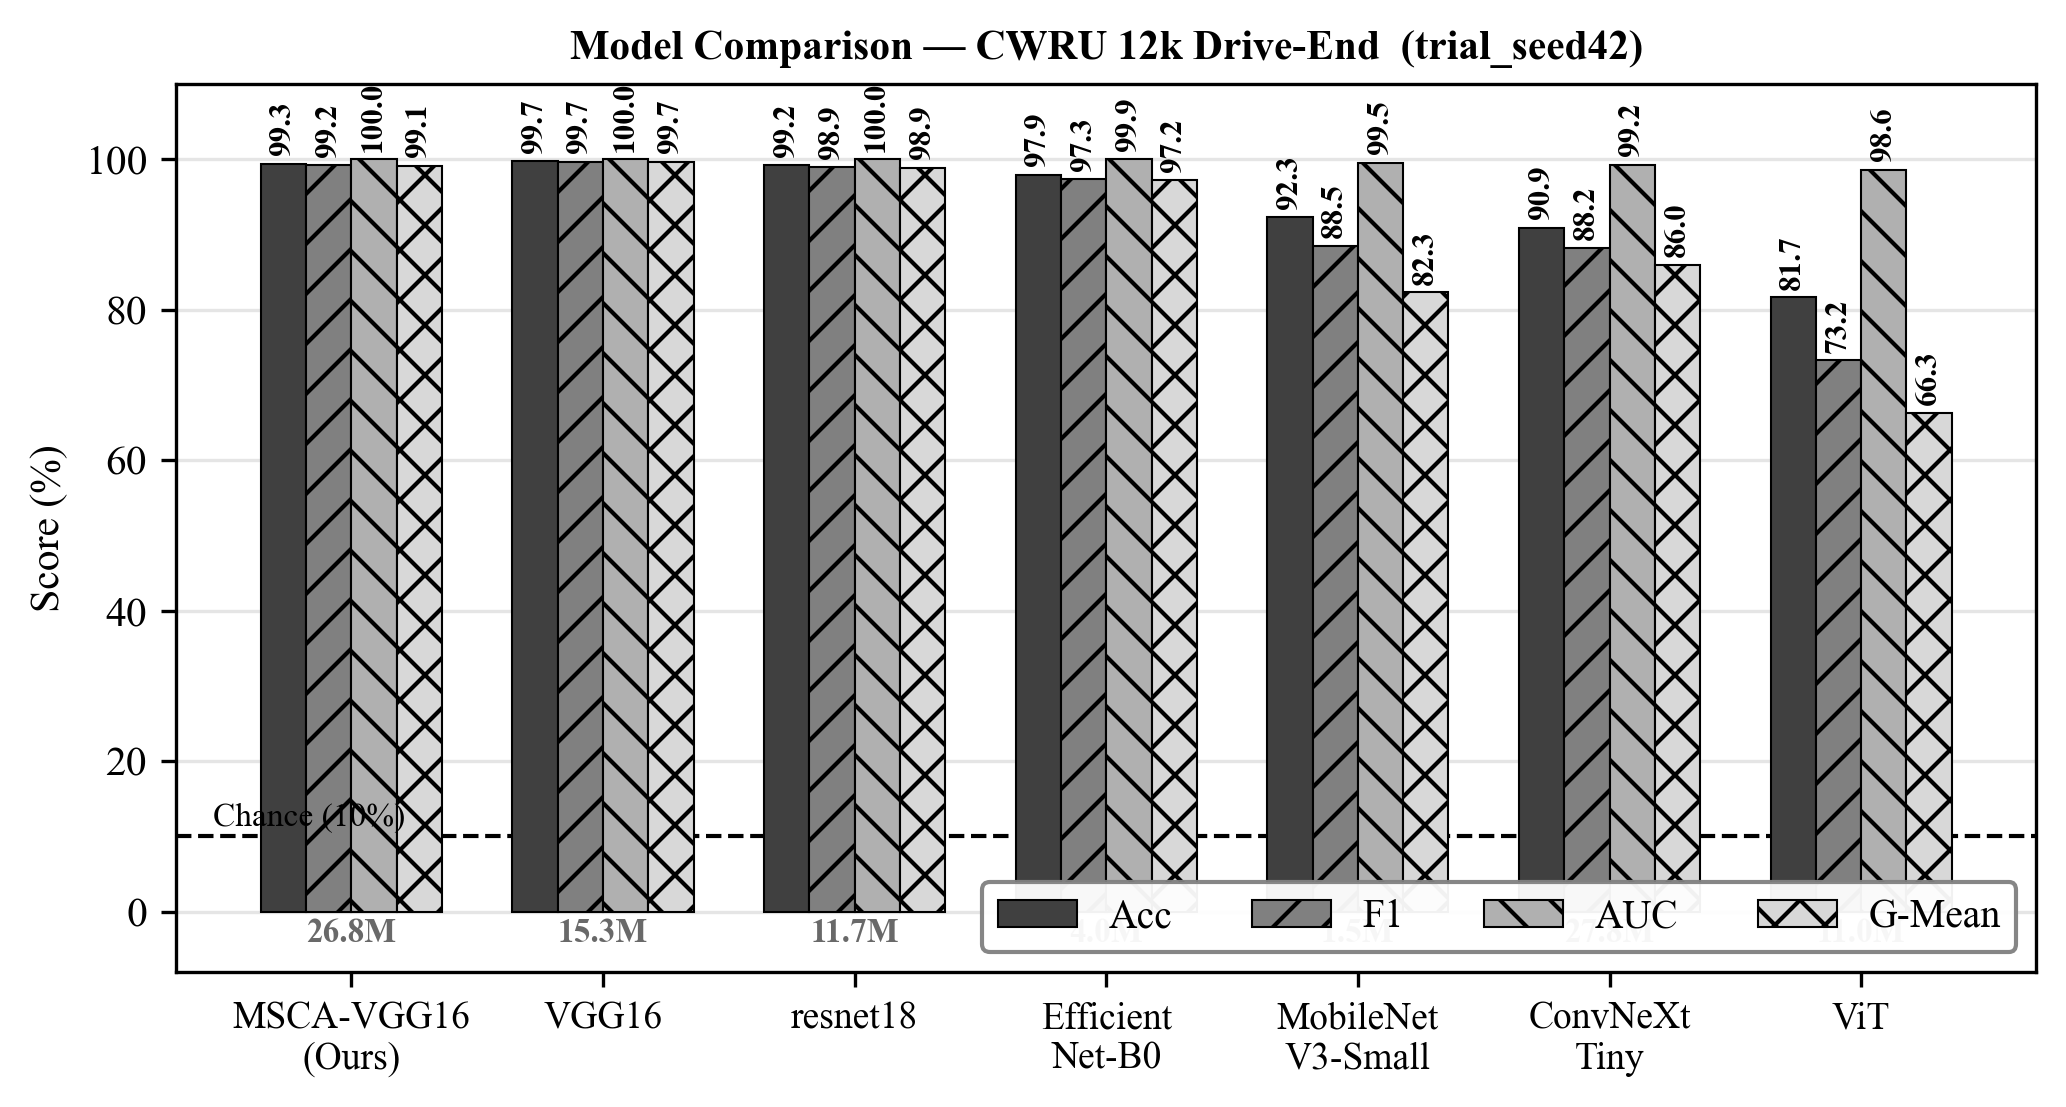
\includegraphics[width=\linewidth]{figures/model_comparison/model_comparison_12k_de_trial_seed42.png}
% \caption{}
% \label{}
% \end{figure*}


% The overall architecture of the proposed MSCA-VGG16 network is illustrated in Fig.~\ref{MSCA-VGG}.
% \begin{figure*}[!htbp]
% 	\centering
% 	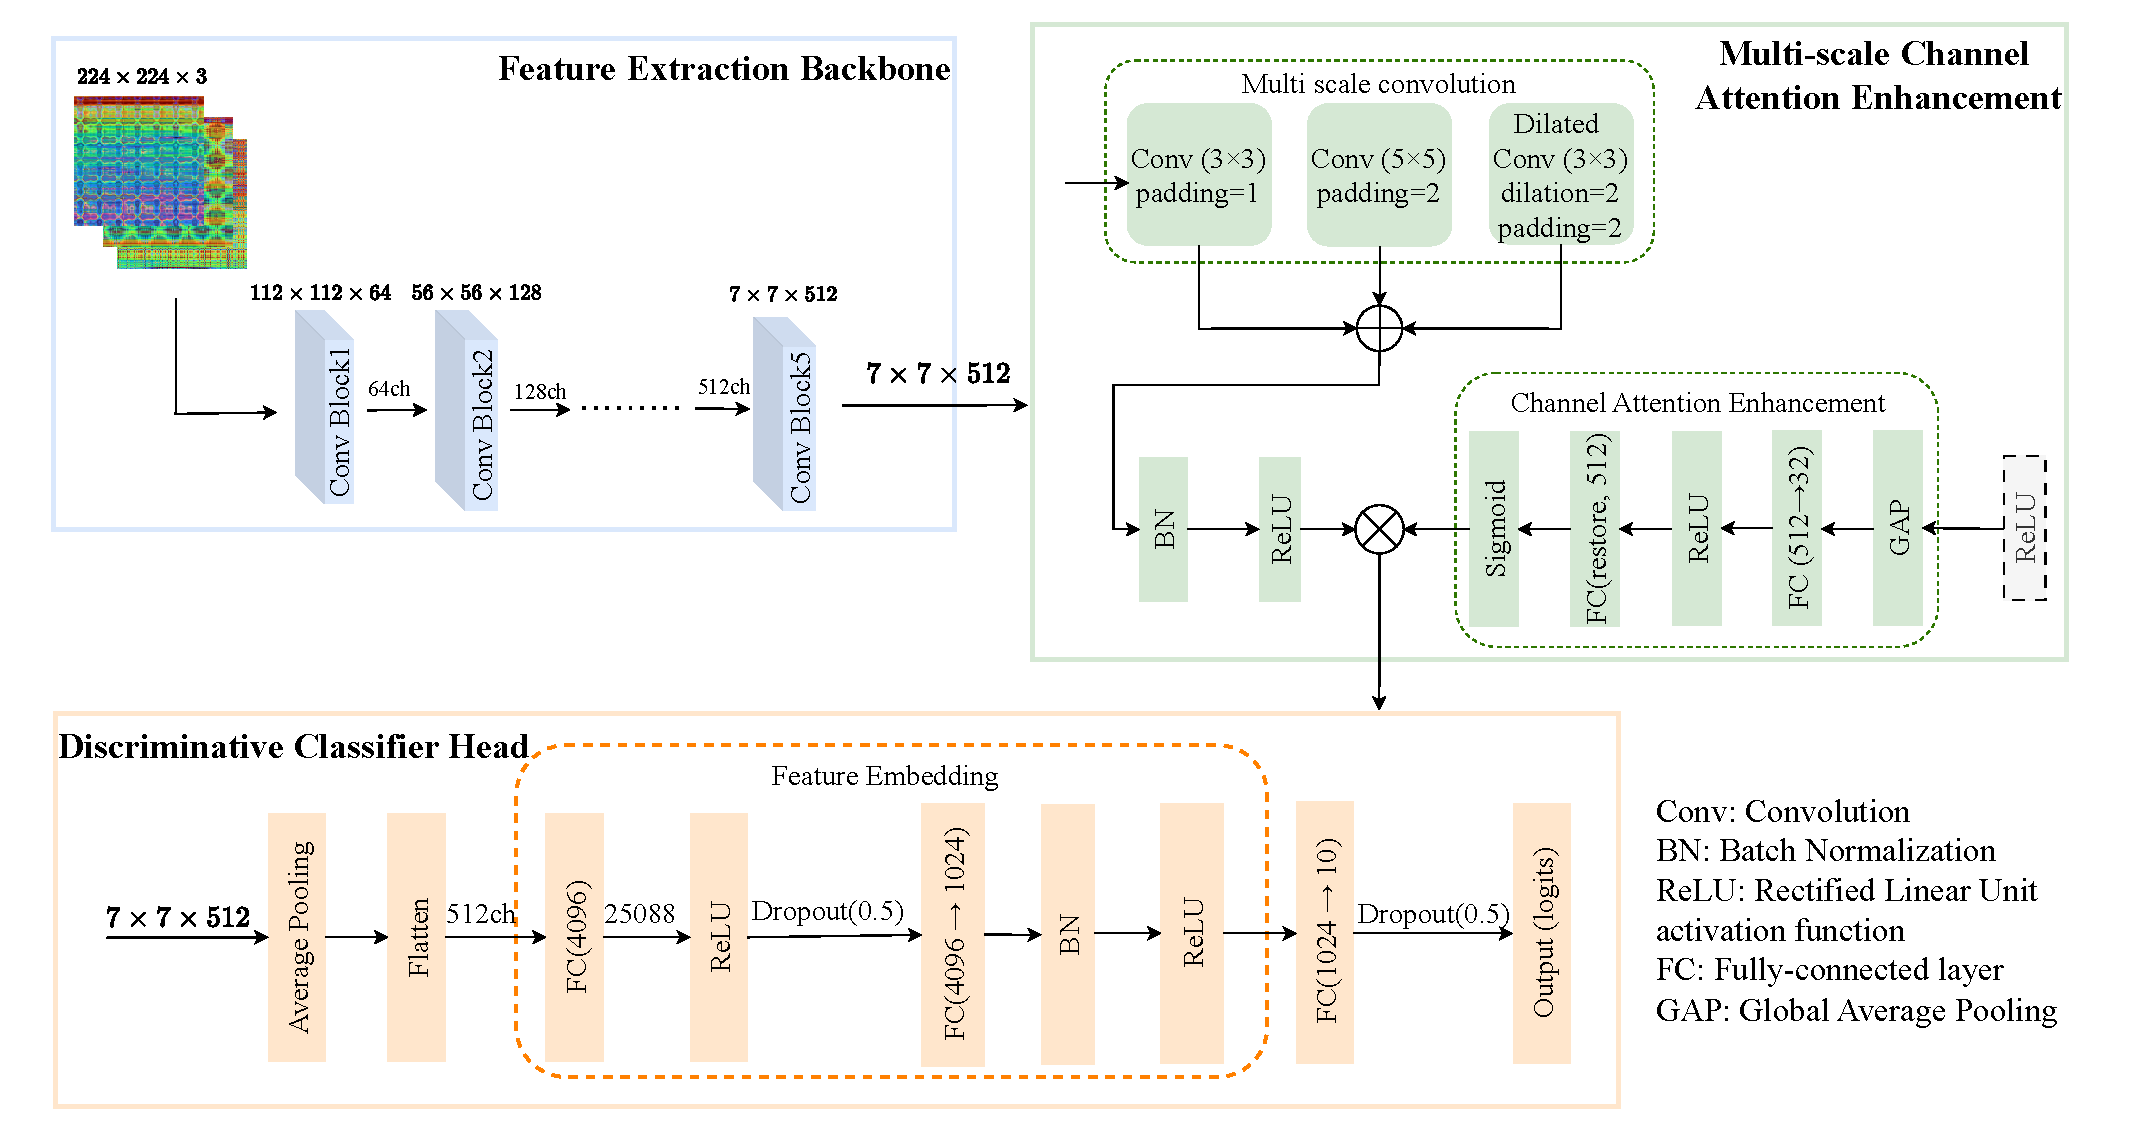
\includegraphics[width=\textwidth]{MSCA-VGG16/MSCA-VGG16}
% 	\caption{Overall architecture of the proposed MSCA-VGG16 network. The fused AW-DPCNN image is processed by a convolutional backbone, followed by a multi-scale convolution module, squeeze-and-excitation channel attention, and a compact embedding head for fault classification.}
% 	\label{MSCA-VGG}
% \end{figure*}


\balance

\bibliographystyle{IEEEtran}
\bibliography{references}

\end{document}